% !TEX root = ../These_TOC.tex
\chapter{Explorer visuellement des données de simulation massives pour analyser le comportement d'un modèle.}
\begin{center}
	{\large Version \hl{2018-09-18}}\\
	\hl{Corrections de la partie 5.1 à 5.2.3 non prises en compte.}

\end{center}
\minitoc

\clearpage

% Plan initial
%\section{Explorati&on manuelle}
%
%\subsection{Paramètres}
%
%\subsection{Indicateurs}
%
%\subsection{Plans d'expérience}
%
%\section{Exploration Systématique}
%
%\section{Scénarios}
%
% Plan détaillé pour demande dérogation 6ème année (2018-05)
%\section{Comprendre un modèle en l'utilisant}
%\subsection{Explorer un modèle en multipliant les simulations}
%\subsection{Explorer le comportement d'un modèle en multipliant les expérimentations}
%\subsection{Explorer en comparant}
%
%\section{Exploration visuelle guidée d'un modèle : analyse de SimFeodal}
%\subsection{Comprendre les variations des paramètres de SimFeodal}
%\subsection{Définir des plans d'expérience pour explorer SimFeodal}
%\subsection{Explorer la variabilité de l'aléa d'un modèle fortement stochastique}
%
%\section{Comprendre un modèle par son exploration systématique}
%\subsection{Compréhension et validation des modèles théoriques}
%\subsection{\textit{Curse of dimensionality} : comment systématiser l'exploration d'un modèle descriptif complexe}
%\subsection{Plan complet vs exploration des possibles}
%
% Plan du 2018-06-12
%

\section*{Introduction}
\addcontentsline{toc}{section}{\protect\numberline{}Introduction}

\hl{A faire}\\
-> Définir notamment la démarche : contraintes générales -> spécificités SimFeodal -> choix méthodos/techniques


\section[Capter les sorties de SimFeodal]{{Capter les sorties de SimFeodal}%
	\sectionmark{Capter les sorties}}\label{sec:sorties-simfeodal}
\sectionmark{Capter les sorties}

Pour évaluer un modèle, on s'appuie sur plusieurs indicateurs de sortie de simulation, de types divers (indicateurs numériques, graphiques, cartographiques etc., \hl{cf. chapitre 3, partie théorique}).
Quand le nombre d'indicateurs devient important, comme c'est le cas dans le modèle SimFeodal (chap 3, partie présentation des indicateurs), la consultation des indicateurs pendant le déroulement d'une simulation devient difficile.
La complexité de ces indicateurs augmente, elle-même, dans le cas d'un modèle stochastique comme SimFeodal, où il est nécessaire de multiplier les réplications afin d'avoir une idée fiable de la tendance du modèle.
Le travail de paramétrage d'un modèle requiert de plus de mener différentes expériences, c'est-à-dire de faire varier les paramètres (chap 4) d'un modèle, démultipliant encore la masse des sorties, et avec elle, la complexité nécessaire à leur étude.
Nous détaillons ici les contraintes qu'entraînent ces différentes spécificités des données issues de simulation de SimFeodal.

	\subsection{Masse des données}
	Dans un premier temps, il convient de noter que l'ensemble des indicateurs observés en sortie de SimFeodal reposent sur des données qu'il est nécessaire de produire et d'enregistrer tout au long de la simulation.
	Ainsi, pour pouvoir tracer une courbe de l'évolution du nombre d'agrégats au cours du temps, encore faut-il avoir accès à cette information, et dès lors, enregistrer, à chaque pas de temps, cette valeur dans un fichier numérique adapté.
	Cette information, en tant que telle, est assez faible, aussi bien en valeur sémantique qu'en valeur prise en mémoire.
	Pour autant, on a montré que les indicateurs de sortie étaient nombreux, et avec eux, la quantité de valeurs à stocker augmente.
	Ainsi, à chaque pas de temps, il faudra enregistrer les valeurs de plusieurs variables.
	Ce comportement est habituel, et un format de données tabulaire se prête bien à un tel enregistrement : une ligne pour chaque pas de temps, et une colonne pour chaque variable à enregistrer.
	On obtiendrait ainsi en sortie de simulation un tableau contenant 18 lignes (le nombre de pas de temps de SimFeodal) et une cinquantaine de colonnes, ce qui serait assez raisonnable.

	Il faut toutefois considérer un aspect important de l'exploration de données issues de simulations : la production de ces données a un coût temporel important, c'est-à-dire que l'exécution d'une simulation requiert un certain temps (3 à 4 minutes pour une exécution du modèle SimFeodal dans la version présentée dans le \hl{chapitre 2}).
	Si l'on considère de plus que les indicateurs peuvent évoluer au cours des étapes de construction et de paramétrage d'un modèle (cf. \hl{encadré chap 3}), on a alors tout intérêt à prévoir ce cas, et donc à enregistrer l'état de variables qui ne seraient pas encore mobilisées pour la production d'indicateurs.
	Dans le cas contraire, pour chaque changement ou ajout d'indicateur, il faudrait relancer des exécutions du modèle sur l'ensemble des jeux de paramètres précédents afin d'être en mesure d'avoir des indicateurs comparables entre les versions.

	Enregistrer l'ensemble des variables d'un modèle est aisé dans le cas d'un modèle théorique simple, par exemple dans le cas d'un modèle comme celui de Schelling (\hl{ref}). Cela se complique quand il s'agit d'enregistrer les variables d'un modèle plus complexe comme SimFeodal.
	Celui-ci comprend ainsi bien plus de variables globales, représentant l'état du système dans son ensemble à chaque instant.
	Surtout, SimFeodal est un modèle qui voit interagir plusieurs types d'agents, chacun situés à différents niveaux de granularité spatiale et sociale.
	Afin d'avoir tous les éléments en main une fois la simulation achevée, il est donc nécessaire d'enregistrer l'ensemble des variables non seulement globales, mais aussi afférentes à chacun des types d'agents.
	D'un tableau de données exhaustif en sortie du modèle de Schelling, on passe donc à plusieurs tableaux, dont les variables respectives seront propres à chaque type d'agent.

	A ce niveau, l'information en sortie est encore relativement contenue : il y a cinq types d'agents, ayant chacun une douzaine d'attributs, dans SimFeodal. On pourrait donc se contenter de ces cinq tableaux contenant 18 lignes (les pas de temps) et la douzaine d'attributs propres, comme c'est classiquement le cas dans (\hl{trouver exemple}).

	Reste encore un obstacle majeur à un enregistrement suffisant du déroulement d'une simulation : une part importante des indicateurs s'appuie sur des données individuelles et non agrégées.
	Ainsi, enregistrer une situation globale des paroisses à chaque pas de temps permet par exemple d'en examiner le nombre, la superficie moyenne ou encore le nombre moyen de paroissiens desservis.
	Mais cela ne permet en aucun cas d'en dresser une cartographie, ce qui nécessite, par définition, d'enregistrer la géométrie de chaque paroisse à chaque pas de temps.
	De même, on a vu que les indicateurs pouvaient être amenés à évoluer : si l'on enregistre un nombre de paroissiens moyen à chaque pas de temps, puis que l'on décide après coup de comparer non plus cette moyenne, mais une médiane, ou encore d'observer la forme de cette distribution, on se trouve alors dans une situation impossible requérant de ré-exécuter les simulations après avoir adapté l'indicateur voulu.

	Pour se prémunir de cette situation, on a donc fait le choix, dans SimFeodal, d'enregistrer les états des variables à des niveaux d'agrégation multiples, y compris au niveau de l'agent individuel. Dans le cas des paroisses, le volume de données résultant reste contenu : on obtient un tableau d'environ 2000 lignes\footnote{
	Avec une moyenne de 120 paroisses, cela représente $18_{\text{\tiny ~[pas de temps]}} \times 120_{\text{\tiny ~[paroisses]}} \approx 2000$ lignes pour chaque simulation.
	} et une dizaine de colonnes\footnote{
	Les identifiants de la simulation (nom, graine aléatoire), le pas de temps, l'identifiant de la paroisse, puis les différents attributs et la géométrie.
	}.
	L'enregistrement systématique de chaque agent est toutefois bien plus gênant dans le cas d'autres agents, par exemple les foyers paysans. Pour ceux-là, et parce qu'on doit être en mesure d'étudier les liens entre satisfactions et choix de déplacements, ou encore d'observer la composition précise de la distribution des satisfactions, il est aussi nécessaire d'enregistrer les attributs de chacun. Avec $4000$ foyers paysans à chaque tour, les données changent ainsi d'ordre de grandeur\footnote{
	$18_{\text{\tiny ~[pas de temps]}} \times 4000_{\text{\tiny ~[foyers paysans]}} \approx 70~000$ lignes pour une exécution du modèle.
	} : chaque simulation requiert de générer un fichier contenant des dizaines de milliers de lignes, pour un total, pour cet unique fichier, d'une dizaine de mégaoctets occupés.

	A terme, pour enregistrer un état représentatif d'une simulation, c'est-à-dire avoir suffisamment d'éléments numériques pour pouvoir générer les indicateurs de sortie et prévoir une partie de leur évolution, la masse de données produite est assez conséquente.

	\subsection{Réplications}

	Comme on l'a vu dans le \hl{chapitre 3}, une simulation ne suffit toutefois pas à évaluer le modèle.
	SimFeodal est ainsi un modèle stochastique, c'est-à-dire qu'une large partie des mécanismes qui l'animent sont basés sur des tirages aléatoires.
	Cet aléa est évident dans les mécanismes faisant appel à un tirage, par exemple le choix de déplacement ou non d'un foyer paysan (\hl{cf. chap2, mécanisme déplacement}).
	Dans le cas de ce mécanisme, un foyer paysan mobile se déplacera selon une probabilité dépendant de sa satisfaction.
	Et s'il y a probabilité, il y a donc aléa.
	Même avec une forte satisfaction --- $0.99$ par exemple ---, il reste donc $1\%$ de chance qu'un foyer se déplace, ce qui, sur un grand nombre de tirages (chaque foyers paysans, à chaque pas de temps), a une forte probabilité de réalisation.
	L'aléa a donc un poids important dans ce type de mécanisme.

	Pour autant, même dans des mécanismes plus anodins, l'aléa est fortement présent, étant au cœur de la conception de SimFeodal.
	Ainsi, le simple ordre d'exécution du mécanisme de déplacement des foyers paysans peut avoir une importance considérable.
	\hl{Cet exemple est faux, en trouver un juste où l'ordre d'exécution importe dans SimFeodal et le développer.}

	On pourrait objecter qu'en considérant les agents de manière agrégée, donc globale, les probabilités s'effectuent sur suffisamment d'individus pour présenter un résultat cohérent et déterministe au niveau de la population dans son ensemble.
	En corollaire, le comportement de chaque agent serait régulé par tant de variables aléatoires qu'on entrerait dans le cadre d'application de la loi forte des grands nombres, les agents adoptant alors en moyenne un comportement proche de l'espérance (moyenne théorique) de chaque tirage.
	Avec ces considérations, on pourrait justifier le déterminisme probable des différentes exécutions de SimFeodal.

	SimFeodal n'est toutefois pas simplement un modèle stochastique, mais avant tout, un modèle complexe, c'est-à-dire s'inscrivant dans le champs des systèmes complexes. Sans vouloir ici entrer dans les détails des implications et raisons de ceci, on peut simplement en retenir, qu'un modèle tel que SimFeodal est extrêmement sensible aussi bien aux conditions initiales qu'aux différents tirages aléatoires.
	\hl{A développer sérieusement ici, ou bien dans les chapitres 1 ou 2. Il faudra de toute façon faire un point quelque part sur les systèmes complexes, l'émergence etc.}
	Pour illustrer, on peut s'appuyer sur un exemple ---
	fictif jusqu'ici dans les différentes exécutions du modèle
	--- possible : à l'initialisation, tous les foyers paysans, placés aléatoirement dans l'espace, seraient ici concentrés dans un espace faible.
	Seul un énorme agrégat émergerait donc, et aucun pôle ne serait susceptible dès lors de diviser cet agrégat géant.
	On atteindrait ainsi une situation très éloignée de l'empirie, et très éloignée aussi des réalisations habituelles du modèle.
	En présence d'un seul agrégat, les possibilités de développement d'attracteurs (châteaux et paroisses) pourraient alors tout aussi bien être fortes que faibles.
	À partir de cette configuration initiale, on ne peut savoir si la situation convergerait vers un agrégat \og paradisiaque\fg{}, extrêmement développé et doté de pôles satisfaisants, ou au contraire, vers un agrégat \og prison \fg{}, où aucun des foyers paysans ne serait satisfait, mais n'aurait non plus d'alternative.

	Cet exemple fictif, volontairement caricatural, ne s'est jamais produit jusqu'ici, mais le cas échéant, encore faudrait-il pouvoir le repérer, pour éventuellement l'isoler d'autres simulations.
	On ne peut donc pas raisonner sur une unique simulation pour évaluer un jeu de paramètres (\hl{cf. chap 3}), mais on ne peut pas non plus se contenter de récupérer des différentes réplications et d'en tirer une moyenne (selon qu'on s'intéresse par exemple à la tendance générale) ou un écart-type (si l'on cherche justement à observer les variations que peut entraîner l'aléa).

	Pour ces raisons, et pour être en mesure d'embrasser l'entière diversité des sorties de simulations issues de variation de la graine aléatoire, il est donc nécessaire de mener plusieurs réplications de chaque simulation, et d'enregistrer l'entièreté des sorties de simulations dans chacun des cas.
	Le jeu de données produit par une simulation, contenant quelques dizaines de milliers de lignes, est ainsi obligatoirement multiplié par le nombre de réplications.
	Pour l'exploration de SimFeodal, après différents tests, ce nombre a été fixé à $20$ réplications (\hl{J'en aurais sans doute parlé dans le chapitre 3 (évaluation), mais à laisser ici jusqu'à ce que ce soit certain.}).
	La dizaine de mégaoctet issue d'une simulation devient donc approximativement 200 mégaoctets, et le nombre de lignes contenues, par exemple pour les foyers paysans, passe d'à peu près $70~000$ à $1~400~000$\footnote{
	Si cette quantité de données semble tout à fait raisonnable et peut largement être traitée sur un ordinateur classique, on peut toutefois noter qu'elle dépasse toutefois déjà le maximum de lignes ($2^{20}, \approx 1~000~000$) que les tableurs classiques ---
	LibreOffice ou Microsoft Excel dans leurs dernières versions en 2018
	--- sont en capacité de gérer.
	}.

	\subsection{Expériences}

	Comme décrit dans le \hl{chapitre 4}, le paramétrage de SimFeodal a demandé plusieurs étapes.
	Chacune de ces étapes représente, qui plus est, plusieurs sous-étapes, faites d'essais et d'erreurs, en faisant varier à chaque fois les valeurs de paramètres de SimFeodal.
	Afin de construire le modèle, puis de l'explorer de manière plus systématique, il a donc été nécessaire de tester des dizaines de configurations de paramètres.
	L'objectif étant de comparer, à chaque fois, les résultats en sortie de simulation d'un nouveau jeu de paramètres testé, il était indispensable de conserver, au minimum, l'ensemble des jeux de données de la version précédemment testée du modèle.

	Cela n'est pourtant pas suffisant, pour plusieurs raisons aussi bien éthiques que méthodologiques.
	En premier lieu, pour des impératifs de reproductibilité (\hl{Ça aussi faudrait quand même en parler quelque part. Chap. 7 ?}) de la démarche engagée, aussi bien que pour la simple capacité à restituer honnêtement et rigoureusement les étapes suivies, il était nécessaire de conserver l'ensemble des indicateurs de sortie de simulations correspondant à chaque étape ou sous-étape.
	Cette démarche de paramétrage s'inscrivant ainsi sur une durée assez étalée, et suivant surtout un avancement non linéaire fait d'allers-retours, il était indispensable de documenter autant que possible chaque avancée, et pour cela, de conserver l'ensemble des résultats en résultant.

	Une autre contrainte, méthodologique, déjà évoquée (\hl{cf. encadré incrémentalité des indicateurs dans chap. 3}), complexifie toutefois encore la tâche.
	Ainsi, les indicateurs jugés utiles évoluent tout au long des étapes de paramétrage.
	Or, pour pouvoir comparer les résultats de simulations issues de jeux de paramètres différents, encore faut-il disposer d'indicateurs comparables, et donc, identiques dans leur définition.
	Si l'on ne conserve que les indicateurs de chaque simulation, on ne peut donc les ajuster sans avoir accès aux données sources ayant permis de les produire.

	Pour ces raisons, il n'était pas possible de mener un travail de paramétrage de SimFeodal sans conserver l'ensemble des données produites, c'est-à-dire l'ensemble des attributs de l'ensemble des agents de chacune des réplications, tout cela pour chacune des expérimentations.

	En supposant que les 8 étapes présentées dans le chapitre précédent (\hl{ref chap2, étapes}) soient ne serait-ce que constituées de 3 sous-étapes chacune --- ce qui est bien en deçà de la réalité ---, on obtient donc 24 jeux de paramètres à stocker, puis à devoir mobiliser.
	Cela représente alors une somme considérable de données, qui se chiffrent en dizaines de millions d'enregistrement\footnote{
	$18_{\text{\tiny ~[pas de temps]}} \times 4000_{\text{\tiny ~[foyers paysans]}} \times 20_{\text{\tiny ~[réplications]}} \times 24_{\text{\tiny ~[jeux de paramètres]}} \approx 35~000~000$ de lignes enregistrées pour les seuls foyers paysans.
	}.
	Si cela ne représente jamais que quelques gigaoctets de données, ce que quiconque a désormais l'habitude de manipuler dans un cadre personnel, en terme de traitement, cette masse de données est à la limite de ce que l'on peut traiter sur un ordinateur individuel.
	Ainsi, selon une approximation courante, on ne peut charger en mémoire de données d'une taille supérieure à la moitié de la mémoire vive disponible, sans même prendre en compte les autres éventuels processus en cours.
	Avec 5 Go de données , il faut donc disposer d'un ordinateur personnel possédant au moins une douzaine de gigaoctets de mémoire vive, et encore, au prix d'un traitement extrêmement lent et bloquant.

	Et encore, on ne mentionne ici que les expérimentations issues des étapes de paramétrage.
	Les phases suivantes d'exploration du comportement du modèle, par exemple autour de variations systématiques de valeurs de paramètres en vue de calibration, demandent ainsi d'exécuter, et donc d'enregistrer, une masse bien plus importante de simulations.

	\subsection{Des données aux indicateurs}\label{subsec:donnees-indicateurs}
	Dans l'ensemble, l'enregistrement et la sauvegarde des données issues de simulations, en vue de leur mobilisation pour produire les indicateurs de sortie, se révèle une contrainte importante dans la compréhension du comportement d'un modèle.
	C'est particulièrement le cas pour SimFeodal, où l'on ne peut se contenter de produire à la volée les indicateurs, pour des raisons de reproductibilité théorique et pratique.

	La masse de données en sortie est impressionnante et requiert donc premièrement d'utiliser des outils adaptés à la manipulation de grands jeux de données.
	Cela exclue de fait l'outillage traditionnel de la géographie quantitative, ne laissant par exemple pas la possibilité d'utiliser les outils à interface graphique classiques.
	Au contraire, face à des données de cet ordre, seules des solutions statistiques, basées sur des analyses en ligne de commande, peuvent être mobilisées.
	Ces solutions doivent en plus être appuyées par des capacités de calculs importantes, sans toutefois justifier encore l'usage de technologies de calcul intensif.
	Cela pose une première contrainte dans l'universalité de l'analyse, en particulier dans un contexte interdisciplinaire porteur d'une large hétérogénéité en matière de pratiques quantitatives : il n'est pas possible de juste envoyer les jeux de données produits aux thématiciens, qui ne pourraient en l'état pas en tirer les indicateurs nécessaires.

	Dans un second temps, et c'est là la contrainte principale, cette masse de données doit servir à la production d'indicateurs, nombreux et divers aussi bien dans leur forme que dans les caractéristiques des processus qu'ils décrivent (\hl{ref. chap. 3, indicateurs}).
	Les mêmes raisonnement que pour les données s'appliquent ainsi aux indicateurs.
	Si on peut prendre en compte la variabilité des réplications directement dans les indicateurs produits (par exemple avec des représentations graphiques de type \textit{box-plot} qu'adoptent une forte partie des indicateurs), ce n'est ni possible ni souhaitable entre les différentes expériences.
	De fait, chaque expérience doit pouvoir être comparée aux précédentes sur la base de leurs seules réplications respectives.
	Dès lors, la raison d'être des indicateurs de sortie est de rendre possible une comparaison, indicateur par indicateur, entre chacune des expériences.
	Il est donc indispensable de générer, pour chaque expérience, l'ensemble des indicateurs. En ne considérant ici encore que 24 expériences, cela fait donc déjà plusieurs centaines\footnote{
	En considérant ainsi une trentaine d'indicateurs, on obtient donc $30{\text{\tiny ~[indicateurs]}} \times 24_{\text{\tiny ~[jeux de paramètres]}} \approx 700$ indicateurs uniques.
	} d'indicateurs (\cref{tbl:hierarchie-simulations}).

	\begin{table}[!]
		\raggedleft
		\resizebox{.85\textwidth}{!}{%
			\begin{tabular}{N|M{2.5cm}|M{2.5cm}|M{2cm}|M{3.5cm}|M{4.5cm}|N|}
				\hline
				&	& \multicolumn{2}{|c|}{\thead{Données}} & \multicolumn{2}{|c|}{\thead{Indicateurs}} \\ \hline
				& \thead{Intitulé} & \thead{Quantité} & \thead{Poids} & \thead{Type} & \thead{Quantité} & \\[25pt] \hline
				\tikzmark{a}& Une simulation & \makecell{$\approx 10^5$ lignes}& $\approx 10$ Mo & \begin{tabular}[c]{@{}l@{}}Visualisations\\ en direct\end{tabular} & \makecell{$\approx 10$ indicateurs}  & \\[50pt] \hline
				\tikzmark{b}& Une expérience & \makecell{$\approx 10^6$ lignes} & $\approx 200$ Mo & Indicateurs de sortie & \makecell{$\approx 30$ indicateurs\\(variabilité des\\réplications)} & \\[50pt] \hline
				\tikzmark{c} & \makecell{Huit étapes\\de\\paramétrage} & \makecell{$\approx ~10^7$ lignes} & $\approx 5$ Go & Indicateurs de sortie & \makecell{$\approx 700$ indicateurs\\ (à comparer entre\\les expériences)} & \\[50pt] \hline
			\end{tabular}%
			\tikz[overlay,remember picture] \draw[->, >=latex', bend right=90, thick, dashed] (a.west) to node[pos=.5, left, align=center, xshift=0pt]{$\times 20$\\$\textrm{réplications}$} (b.west) ;
			\tikz[overlay,remember picture] \draw[->, >=latex', bend right=90, thick, dashed] (b.west) to node[pos=.5, left, align=center, xshift=0pt]{$\times \approx 24$\\$\textrm{expériences}$} (c.west) ;
		}
		\caption{Synthèse de la multiplication des données et indicateurs selon la hiérarchie des simulations.}
		\label{tbl:hierarchie-simulations}
	\end{table}

	Le choix ayant été fait de mener une comparaison visuelle (\hl{ref. dans chapitre 3 : indicateurs uniques vs fonctions objectifs}), on imagine dès lors que celle-ci va être difficile en présence de tant d'indicateurs.

	En sus de la contrainte de l'enregistrement et de la production des indicateurs, le verrou majeur à la compréhension des phénomènes modélisés dans SimFeodal est donc la simple capacité à visualiser et à explorer l'ensemble des indicateurs de sortie.
	Ce qui doit de plus être rendu accessible y compris pour un auditoire non habitué à la manipulation de nombreuses données et sorties quantitatives.

\clearpage
\section[Explorer les sorties]{Comment explorer les données de SimFeodal ?}\label{sec:explorer-sorties-simfeodal}

	Pour évaluer une expérience de SimFeodal, on doit passer en revue une trentaine d'indicateurs de sortie de simulation.
	Cette évaluation ne vise pas à aboutir à une note unique, mais plutôt à une idée de la capacité de l'expérimentation à reproduire les dynamiques modélisées.
	Il ne s'agit donc pas a proprement parler d'une évaluation du modèle, mais plutôt d'une exploration de son comportement en fonction des mécanismes et valeurs de paramètres choisis.
	Pour mener cette exploration, il convient d'utiliser des outils adaptés, c'est-à-dire de disposer de solutions techniques permettant le calcul et l'affichage des indicateurs à partir des données produites par le modèle.
	Dans le travail mené autour de SimFeodal, plusieurs solutions ont été utilisées au cours des différentes étapes de construction du modèle.
	La restitution purement chronologique de ces solutions ne revêt pas d'intérêt propre, mais les contraintes accumulées au cours de la construction du modèle et les choix devant permettre de les dépasser nous paraissent très largement génériques.
	Nous justifions donc ici la succession de choix d'outils d'explorations au prisme des verrous dans l'exploration que chacun a permis de débloquer, ce qui dresse par là-même un portrait des solutions méthodologies d'exploration de données de simulations dont on peut faire usage selon les contraintes générales des modèles.\hl{Pas clair, à reprendre, mais l'idée est là.}

	\subsection{Observation en direct vs a posteriori}\label{subsec:observation-a-posteriori}

	Classiquement, le premier réflexe d'un modélisateur, du moins pour les modèles à base d'agents, est de définir des sorties graphiques pour accompagner son modèle.
	Les différentes plate-formes de modélisation agent mettent d'ailleurs régulièrement en avant les possibilités de représentations qu'offrent leurs environnements (\hl{ref blogs Gama, NetLogo 3D, GeoMASON, Repast}).
	Visualiser le déroulement d'un modèle \og en direct\fg{} (\textit{online} dans \cite{grignard_agent-based_2017}) offre ainsi de nombreux avantages (\hl{cf. HDR Arnaud, en sortir une citation et/ou un listing}).

	Dans l'exploration de SimFeodal, la création en direct de quelques graphiques correspondant à des indicateurs étudiés permet de vérifier, avant le lancement d'une série de simulations, que le déroulement de la simulation ne présente pas de forte incohérence et qu'un \textit{bug} n'a pas été introduit involontairement.
	Pourtant, deux contraintes limitent fortement le recours à ce type de visualisation en direct des simulations.

	La première contrainte, déjà évoquée plus haut, est que le modèle SimFeodal est fortement stochastique.
	Dès lors, la visualisation des indicateurs d'une simulation particulière ne suffit pas à estimer le comportement du modèle.
	C'est bien pour cela que les indicateurs choisis pour l'évaluation de SimFeodal prennent presque tous en compte la variabilité des résultats induite par l'exécution de réplications.

	Certains environnements techniques (\hl{ref à multi-simulation dans Gama}) permettent toutefois de mener concomitamment plusieurs réplications d'un même modèle et de visualiser directement pendant l'exécution les résultats des réplications agrégés.
	La première contrainte, liée à la nécessaire étude des réplications du modèle, peut donc être dépassée en adaptant l'implémentation du modèle pour faire usage de ces capacités de multi-simulation.

	La seconde contrainte est plus cruciale dans le cas de SimFeodal et invalide l'usage des méthodes de visualisation en direct.
	On l'a vu, l'exploration des sorties de simulation du modèle repose sur la consultation d'une trentaine d'indicateurs, parfois très spécifiques au cas d'étude de SimFeodal.
	Outre le fait qu'il serait concrètement difficile de représenter tous ces indicateurs au sein de l'interface graphique d'une plate-forme de simulation agent, la temporalité de l'exécution d'une simulation (ou même des réplications nécessaires) est bien plus courte que celle requise pour la compréhension des résultats produits.
	Les indicateurs de sortie de simulation demandent ainsi un examen approfondi avant d'être en mesure de juger de leur adéquation aux attentes thématiques.
	Cet examen ne peut que difficilement être réalisé en direct, qui plus est quand il demande de faire appel, dans le cadre de co-construction inhérent à SimFeodal, à plusieurs points de vue.
	Les modalités mêmes de l'exploration des sorties de SimFeodal requièrent donc que les indicateurs soient visibles et explorables à des temporalités différentes, par des chercheurs différents, depuis des lieux différents.
	Pour un même chercheur, l'évaluation n'étant pas une étape unique et finie, il est utile de pouvoir revenir sur les résultats à différents moments, ne serait-ce que pour comparer les nouveaux résultats produits à ceux générés par des expérimentations précédentes.

	Il est donc indispensable que les indicateurs soient enregistrés et consultables simplement à tout moment, ce qui élimine de fait la visualisation des indicateurs en direct pendant l'exécution des simulations comme unique méthode d'exploration du comportement de SimFeodal.

	La visualisation en direct n'est donc pas mobilisable en tant que telle, mais elle peut tout de même, comme dans un usage très classique, être utilisée comme un outil de validation interne pour tester chaque modification dans les valeurs de paramètres.
	Visualiser une seule simulation, avant d'en exécuter les réplications nécessaires, permet ainsi déjà de vérifier que les modifications apportées dans les valeurs de paramètre ou dans les mécanismes n'ont pas entraîné l'apparition de \textit{bugs} ou d'incohérences immédiatement visibles.

	Nous avons donc choisi de doter SimFeodal d'une interface graphique, très sommaire, mais permettant des allers-retours rapides entre l'implémentation et l'exécution.
	Cette interface n'affiche qu'un nombre réduit d'indicateurs (\autoref{fig:simfeodal_gui_indicateurs}), ainsi qu'une représentation cartographique (\autoref{fig:simfeodal_gui_carte}) utile à une analyse rapide du comportement d'ensemble du modèle.

\begin{figure}[H]
	\captionsetup{width=\linewidth}
	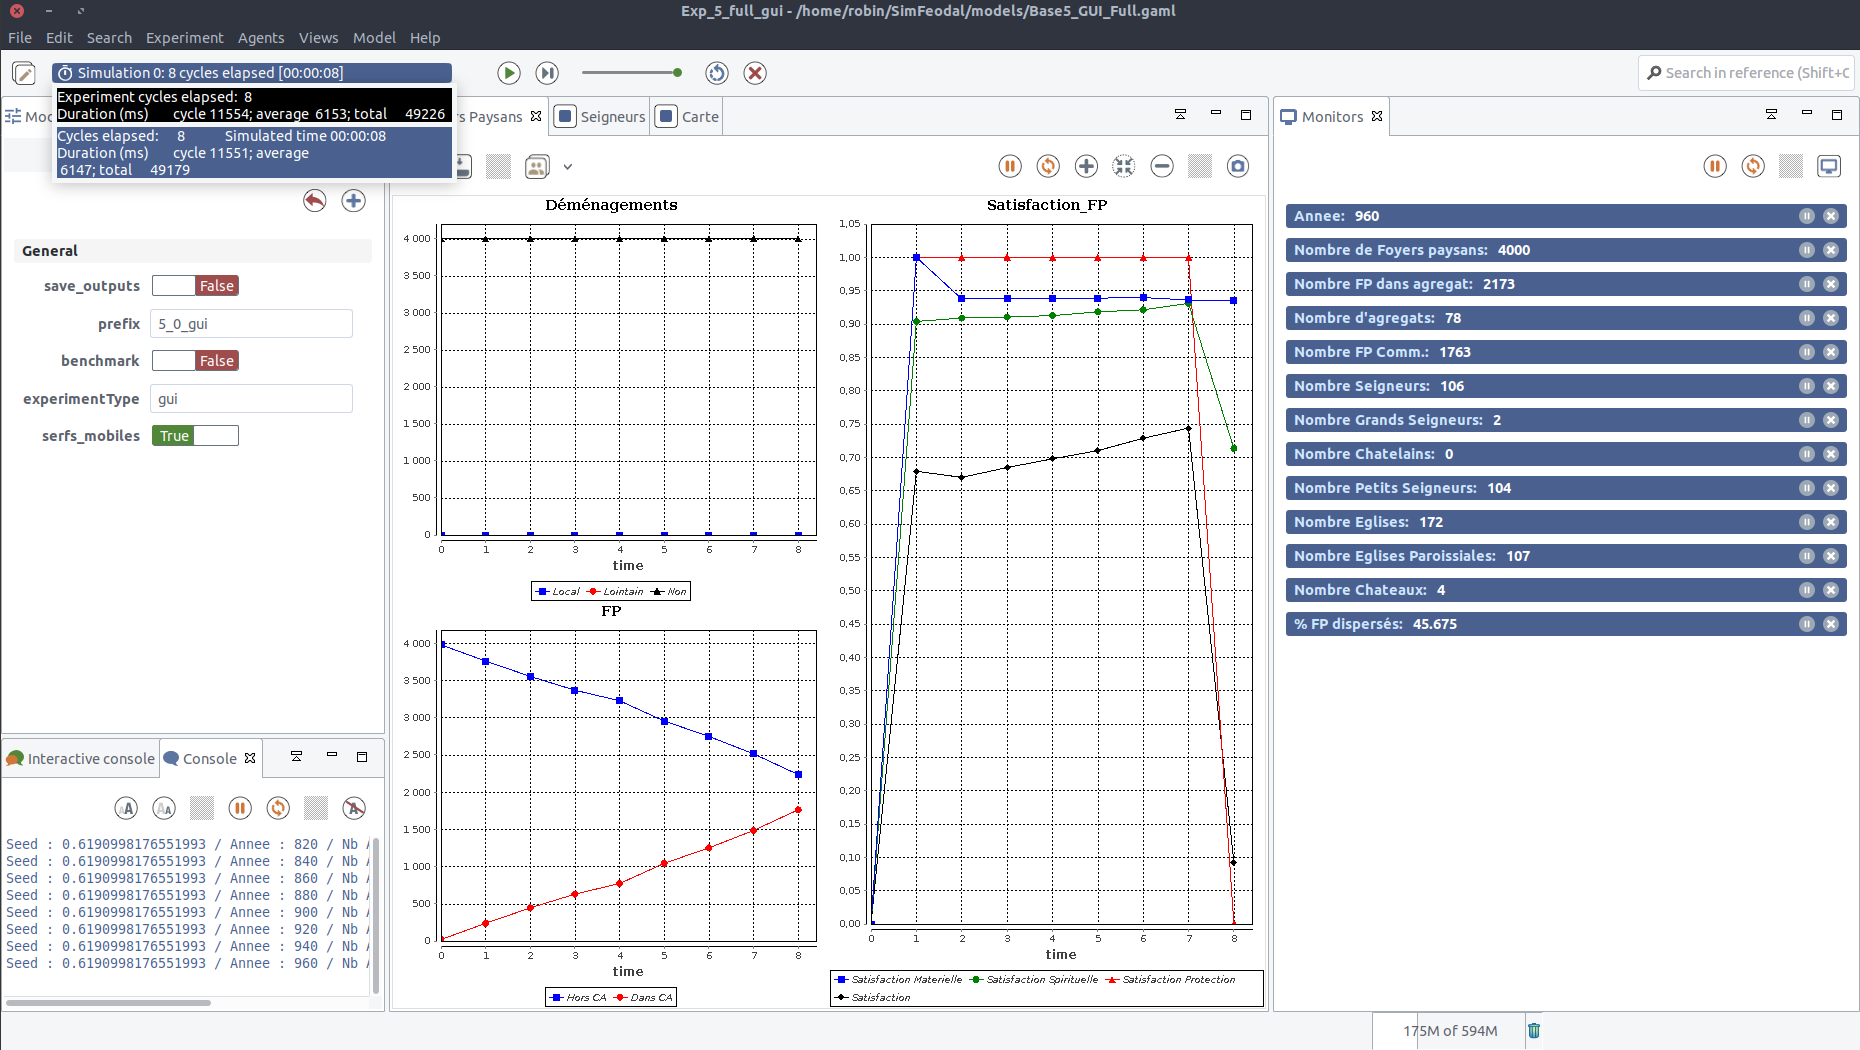
\includegraphics[width=0.5\linewidth]{img/SimFeodal_GUI_FP.png}
	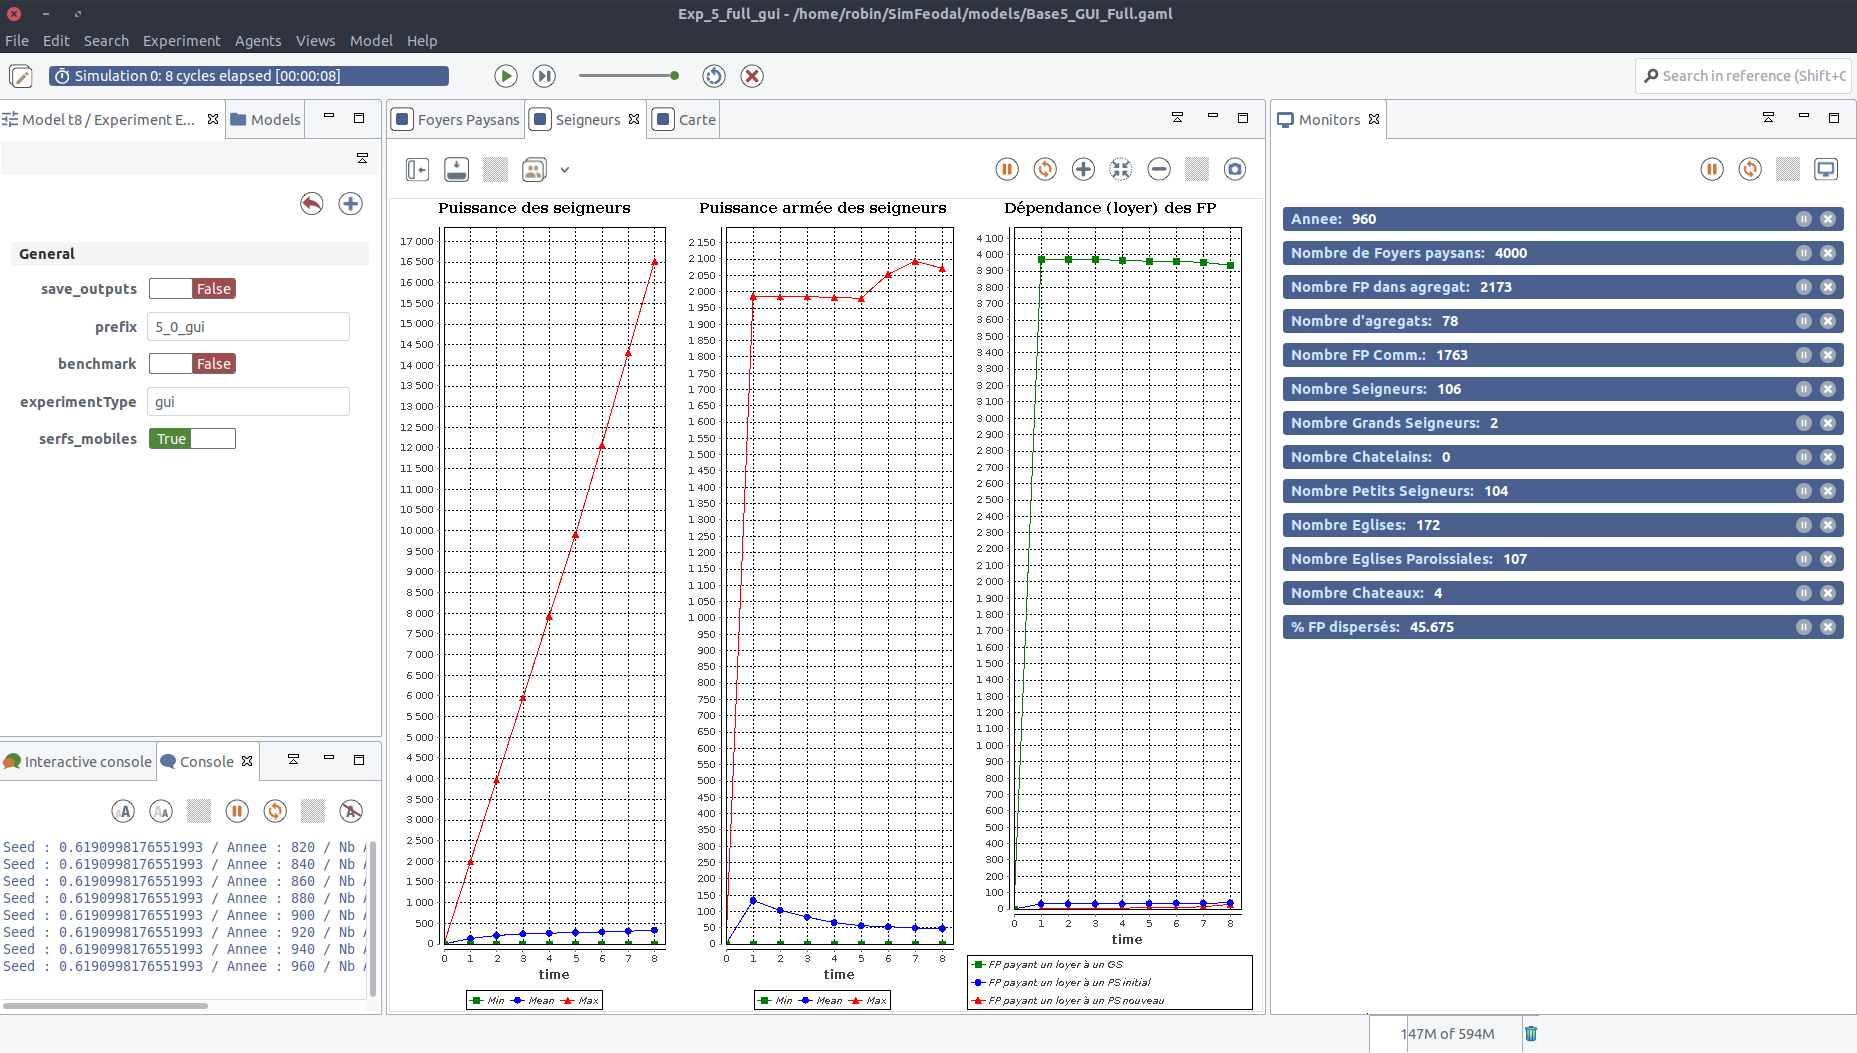
\includegraphics[width=0.5\linewidth]{img/SimFeodal_GUI_seigneurs.png}
	\caption{Visualisations intégrées à l'interface graphique de SimFeodal : indicateurs liés aux foyers paysans et aux seigneurs.}
	\label{fig:simfeodal_gui_indicateurs}
\end{figure}

\begin{figure}[H]
	\captionsetup{width=\linewidth}
	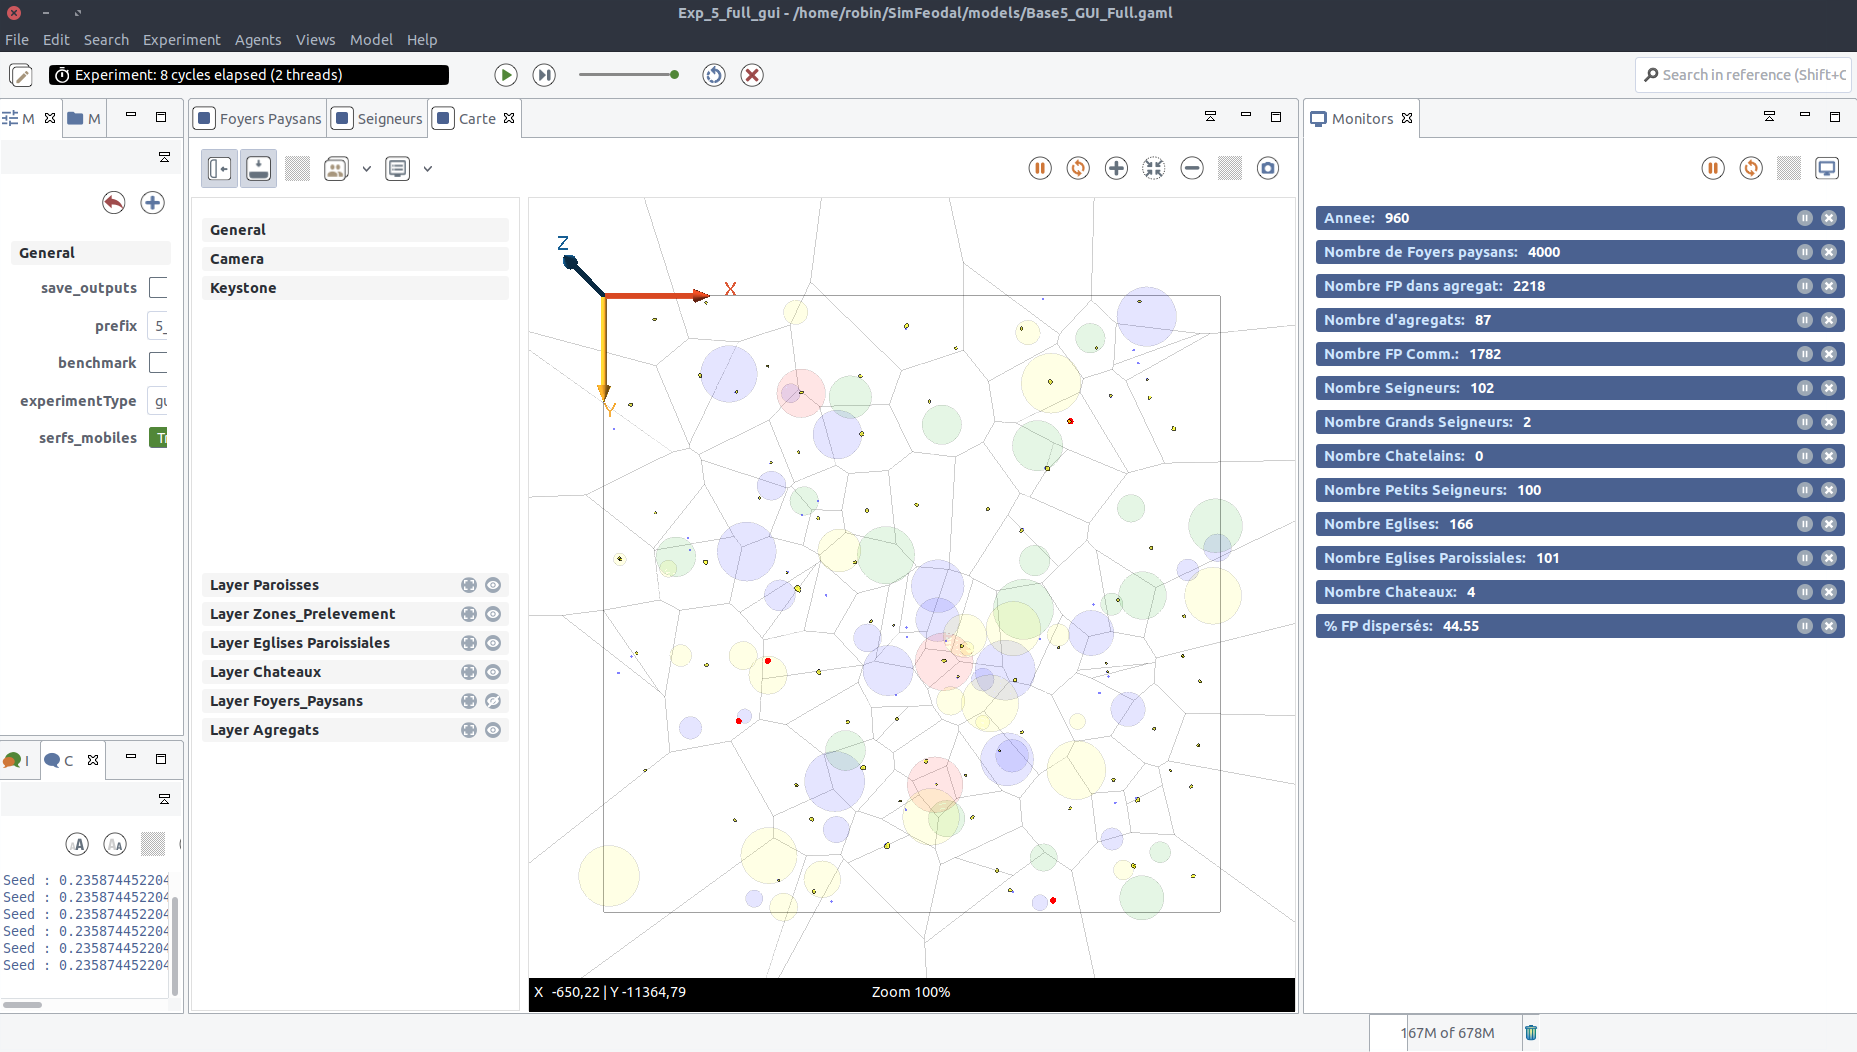
\includegraphics[width=\linewidth]{img/SimFeodal_GUI_carte.png}
	\caption{Visualisations intégrées à l'interface graphique de SimFeodal : cartographie synthétique de l'espace modélisé.}
	\label{fig:simfeodal_gui_carte}
\end{figure}

	Ces représentations ne suffisent pas et ne remettent aucunement en cause les constats de leur inadéquation aux contraintes d'ensemble de l'évaluation de SimFeodal.
	Elles complètent cependant la démarche d'évaluation du modèle par l'ajout d'une étape de contrôle préalable au lancement d'expériences,ce qui ne peut être qu'avantageux.

	\subsection{Générer les indicateurs}

	Si la production des indicateurs doit donc nécessairement être réalisée en aval de l'exécution des simulations (\textit{offline} dans \cite{grignard_agent-based_2017}), encore faut-il disposer d'outils adaptés au traitement des données produites, c'est-à-dire répondant aux contraintes identifiées auparavant (\autoref{subsec:donnees-indicateurs}).
	La contrainte principale est d'être en mesure de gérer la masse de données produites.
	On l'a vu, cela élimine d'office les outils de type tableurs, ou encore les outils de manipulation graphique de données les plus courants.
	Pour les raisons évoquées dans le chapitre 1 (\hl{Positionnement : pourquoi utiliser des outils libres ?}), seules les solutions techniques non-propriétaires étaient envisageables.

	Certains outils graphiques, basés sur des logiciels libres en arrière-plan (PSPP, R Commander, Orange), sont extrêmement aisés à prendre en main et auraient pu constituer un bon choix.
	Pourtant, avec une trentaine d'indicateurs à produire pour chaque expérience, donc de manière régulière, nous avons préféré nous tourner vers des outils plus orientés vers une interface en ligne de commande (\textit{Command Line Interface}, abrégés \textit{CLI}).

	L'utilisation de CLI a plusieurs intérêts gravitant autour de la reproductibilité des traitements.
	En premier lieu, ils permettent une adaptation aisée et rapide aux différents jeux de données.
	Ainsi, partant du principe que les données générées par les réplications et expérimentations sont de même structures, il suffit généralement de modifier le chemin d'entrée des fichiers résultants pour reproduire à l'identique une analyse sur un nouveau jeu de données.

	De manière plus technique et interne à la génération des indicateurs, on peut remarquer que les différents indicateurs de sortie de simulation choisis présentent souvent des caractéristiques communes, aussi bien dans le traitement nécessaire que dans les formats (graphiques) produits.

	Par exemple, la grande majorité des indicateurs reposent sur une première agrégation des données par réplication et pas de temps simulé, puis par une seconde agrégation montrant la variabilité des situations générées, au niveau de l'expérimentation donc.
	En terme de manipulation de données, seul l'indicateur statistique final, et éventuellement l'agent caractérisé, est ainsi modifié dans ces nombreux indicateurs de sortie.
	Le recours à des traitements en CLI permet ainsi un simple copier/coller, voir la création de fonctions dédiées, pour effectuer ces traitements très récurrents.

	Au niveau des sorties graphiques, et donc des indicateurs multi-dimensionnels (\hl{cf. chap 3 et schéma des indicateurs}), on peut aussi remarquer que la forme est assez largement identique : on représente les pas des temps (les années simulées) en abscisse, un indicateur statistique en ordonnée, et les figurés sont sous forme de \textit{box-plot} minimalistes (\og \textit{minimal boxplot}\fg{}, promus par Edward Tufte pour minimiser le ratio données-encre.\hl{Mettre les réfs de Tufte}).
	Là aussi, en disposant d'un environnement de type CLI, et qui plus est en faisant usage de solutions graphiques construites sur une syntaxe régulière et générique\footnote{
	On utilise pour tous ces graphiques le \textit{package} R \texttt{ggplot2}, qui repose sur la grammaire graphique conçue par Leland Wilkinson (\hl{ref}).
	}, il devient très confortable de n'avoir qu'a adapter un premier graphique conçu aux autres indicateurs souhaités.

	Avec ces solutions, il est facile de concevoir et d'implémenter les codes informatiques nécessaires à la génération des indicateurs de sortie de simulation.
	Cela est de plus, dans l'exécution de ces programmes, extrêmement rapides, les différents fichiers de sortie de simulation étant lus et parcourus un unique fois pour en tirer toutes les variables nécessaires à l'établissement des indicateurs.

	En sortie, on obtient une table synthétique (indicateurs numériques, \hl{cf. schéma chap. 3}) et de nombreux graphiques dans des formats vectoriels, donc aisément modifiables, par exemple pour publication, et surtout, lisibles et transférables très simplement.

	\subsection{Organiser les indicateurs en rapports paramétrables}

	Du point de vue de la manipulation, la création de fichiers informatiques indépendants correspondant aux différents indicateurs de sortie de simulation est extrêmement pratique : on peut facilement les échanger et les adapter, par exemple pour inclusion dans une publication.

	Du point de vue de la comparaison des résultats, cette forme n'est pourtant pas la plus adaptée.
	Si l'on peut facilement comparer un même indicateur portant sur deux expériences différentes, la tache se complique quand il s'agit d'avoir une vision globale des différences dans les indicateurs entre deux expériences.
	Pour cela, la démultiplication des fichiers correspondant aux indicateurs se révèle rapidement être un obstacle : on est alors amené à jongler entre de très nombreux fichiers.

	Pour rendre la comparaison des indicateurs plus aisée, en présence d'une forte diversité d'indicateurs, il convient donc, a minima, d'organiser les indicateurs.
	Nous entendons ici par organisation, une présentation structurée, suivant un certain ordre, identique selon les expériences, adapté à une évaluation des résultats du modèle SimFeodal.
	Pour cela, nous avons choisi d'organiser ces \og indicateurs\fg{} au sein de \og rapports \fg{}.
	Cela permet, dès lors que les expériences simulées ont été nombreuses, de rassembler l'ensemble des indicateurs de sortie propres à chacune dans un unique fichier, à la structure toujours similaire.

	En dehors du simple archivage des sorties, la production de rapports facilite aussi la comparaison des expériences par le biais de leurs indicateurs de sortie.
	On peut ainsi, par exemple, placer côte à côte deux rapports rendant compte de deux expériences différentes, et, en les faisant défiler simultanément, comparer point par point, c'est-à-dire indicateur par indicateur, leurs résultats respectifs.

	Les formes que peuvent prendre des rapports, tout autant que les modalités de leur production, sont multiples et extrêmement diverses, depuis le document produit manuellement en insérant des bons indicateurs au fur et à mesure, par exemple dans un traitement de texte, jusqu'au rapport entièrement automatisé produisant des commentaires automatiques des indicateurs insérés en fonction d'expressions conditionnelles.

	Pour SimFeodal, nous avons choisi de restreindre au maximum la manipulation manuelle, c'est-à-dire de générer un rapport entièrement automatique, ne requérant pas d'action spécifique en dehors du choix des données depuis lesquelles créer les indicateurs et donc le rapport.
	Le rapport produit (\cref{fig:simfeodal_rapport_mini} pour un aperçu global, et \hl{annexe X pour un exemple de rapport complet}) n'intègre ainsi que les indicateurs, c'est-à-dire les indicateurs numériques -- sous forme de tableau -- et les indicateurs multi-dimensionnels -- sous forme de graphiques --.
	Ces indicateurs sont toutefois organisés par partie, en l'occurrence par le type d'agents et de comportement qu'ils décrivent.

	\begin{figure}[H]
		\captionsetup{width=\linewidth}
		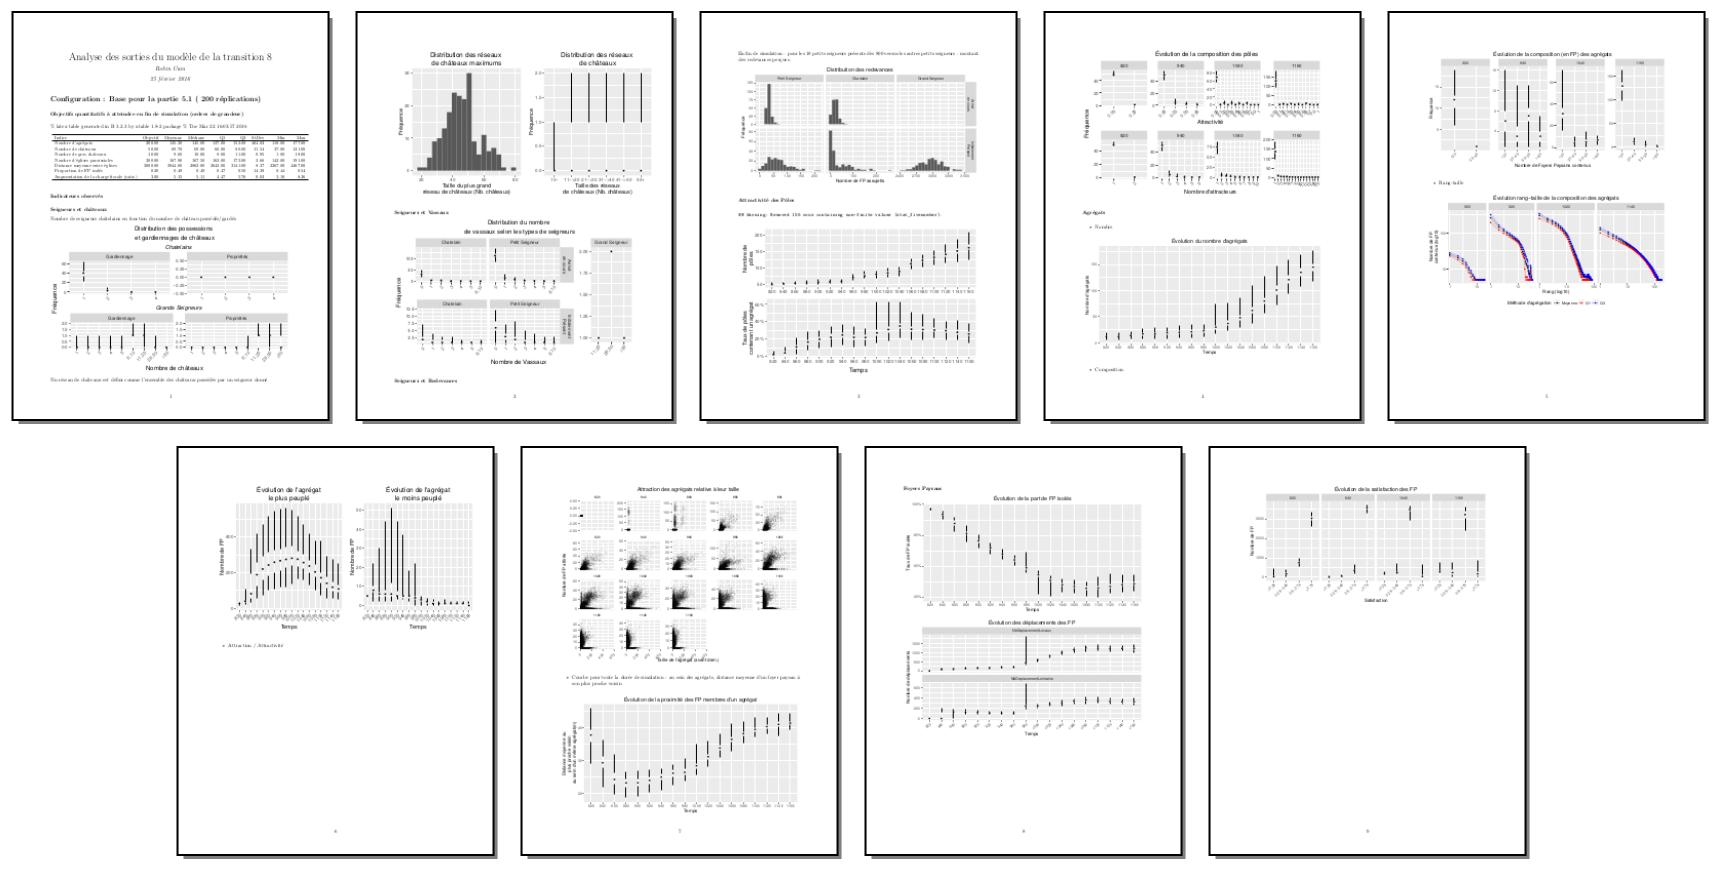
\includegraphics[width=\linewidth]{img/SimFeodal_Rapport_exemple.png}
		\caption{Un exemple de rapport automatique généré pour une expérimentation (étape 0) de SimFeodal. La version en taille réelle est reproduite en \hl{annexe X}.}
		\label{fig:simfeodal_rapport_mini}
	\end{figure}

	Les raisons de ce choix sont multiples, mais ont en commun une recherche de reproductibilité des résultats et des analyses menées.
	Reproductibilité certes théorique (\hl{encore une ref au positionnement}), les résultats de simulation devant être en mesure d'être analysés et reproduis par de potentiels intéressés, mais reproductibilité aussi rendue nécessaire par la pratique de la modélisation, tel qu'explicité auparavant (\hl{ref. à partie 1 du chap, dans réplication -> expériences}).
	La quantité d'expériences requises pour arriver à un état satisfaisant de SimFeodal a ainsi été importante, et le nombre de rapports tout autant.
	La création d'un rapport automatisé garantissait d'une part une génération rapide des indicateurs sur les nouvelles données, permettant donc un examen des sorties de simulation presque immédiatement après leur exécution.
	D'autre part, la structure assez fixe d'un rapport automatisé, c'est-à-dire se basant une structure de données figée (des fichiers tabulés dotés d'en-têtes constantes), ou encore sur une masse suffisante et nécessaire de réplications (pour que les indicateurs soient comparables, ils doivent être réalisés sur le même nombre de réplications, $20$ dans notre cas, ce qui est introduit comme contrainte dans la génération du rapport), permet une première évaluation du bon déroulement \og interne \fg{}\footnote{
	Au sens de l'évaluation interne, c'est-à-dire du bon fonctionnement, exempt de \textit{bugs}, du modèle de simulation implémenté.
	} de la simulation : si le rapport ne peut être généré, c'est que le modèle a été modifié d'une manière qui le rend non rétro-compatible, du moins en ce qui concerne ses sorties.

	Un autre intérêt majeur des rapports, déjà pointé en avantage des outils de type \textit{CLI} est leur adaptabilité.
	On a vu (chap. 3) que les indicateurs à examiner sont nombreux et surtout, évolutifs, dans le sens où ces indicateurs ont fortement été modifiés, remplacés, affinés, au cours des étapes de paramétrage de SimFeodal.
	L'utilisation de rapports automatique permet de changer le code source, qui permet de générer les indicateurs, en un unique endroit.
	À partir de là, pour mettre à jour l'ensemble des rapports déjà produits, c'est-à-dire regroupant les indicateurs de chacune des expériences passées, il suffit de ré-exécuter la routine de production des rapports, ce qui représente un gain de temps et d'efficacité conséquent dans les situations de changements fréquents d'indicateurs, comme cela a été le cas pour SimFeodal.


%	\begin{encadre}{Générer les rapports avec \texttt{R} et \texttt{knitr}}{enc-technique-rapports-knitr}
%
%		\hl{Encadré sur les rapports automatiques, le \textit{\og litterate programming}\fg, le choix et le paramétrage de knitr + lien vers le code-source des rapports.}
%
%	\end{encadre}


	Naturellement, la reproductibilité des rapports constitue plus un objectif qu'une réalisation effective.
	Ainsi, comme explicité dans l'encadré sur l'incrémentalité des indicateurs (\hl{ref encadré incrémentalité chap 3}), une contrainte forte empêchent une absolue reproductibilité des analyses du comportement des différentes versions de SimFeodal : les données générées par les différentes versions du modèle ne sont pas systématiquement \og compatibles \fg{}, c'est-à-dire qu'elles ne présentent pas toute exactement la même structure, à commencer par les variables enregistrées.

	Dès lors, les différents rapports peuvent être considérés comme reproductibles et automatiques au sein de \og générations \fg{} de SimFeodal, c'est-à-dire pour les versions créées et paramétrées dans le cadre d'une même phase de co-construction, avant donc d'avoir eu à adapter les indicateurs\footnote{
	\hl{Pas clair du tout, à reprendre !}
	}.

	A l'issue de la conception et de l'implémentation de ces rapports automatiques, on dispose donc, pour chaque expérience, d'un document aisément partageable et lisible.
	Ce pourrait être la dernière étape de la création d'outils d'évaluation de SimFeodal si le nombre de versions ou d'étapes de SimFeodal était plus restreint.
	Pourtant, comme vu dans \hl{la partie 1 du chapitre}, le paramétrage de SimFeodal a été caractérisé par une forte quantité d'allers-retours entre le modèle et ses résultats, entraînant à chaque fois de nouvelles expérimentations.
	De la même manière qu'au regard du nombre d'indicateurs à évaluer il n'est donc pas possible de manipuler les indicateurs un par un dans des fichiers individuels, la masse d'expériences rend partiellement caduque l'utilisation unique des rapports automatiques.
	Il est facile de comparer, sur un même écran d'ordinateur, deux ou trois rapports, mais dès lors qu'il faut en comparer plus que cela, la manipulation conjointe des rapports devient complexe, tout autant que d'avoir une vision globale des résultats principaux de chaque expérience.

	\subsection{Organiser les rapports : Dashboards}\label{subsec:dashboards}

		%%%%%%%%%%%%%%%%%%%%%%%%%%%%%%%%%%%%%%%%%
	\begin{center}
		\hl{Sous-sous partie complètement reprise}\\
		\hl{LENA : A lire à partir d'ici.}
	\end{center}
	%%%%%%%%%%%%%%%%%%%%%%%%%%%%%%%%%%%%%%%%%

	Pour être en mesure de comparer de nombreux éléments, il est nécessaire de passer d'une exploration linéaire, fondée sur le visualisation successive de chacun des indicateurs, à une exploration globale et interactive.
	En pratique, plutôt que de faire défiler visuellement les nombreuses pages d'indicateurs, mieux vaut une interface présentant les points clefs de l'évaluation et qui permette d'entrer dans le détail de chacun des indicateurs après-coup.

	\subsubsection{Les \textit{dashboards}}

	Cette logique, assez universelle désormais, est celle qui préside à la création des nombreux \og tableaux de bord \fg{}, ou \og \textit{dashboards} \fg{} que l'ont voit émerger depuis la fin des années 1990.
	Rob Kitchin et ses co-auteurs définissent ainsi les \textit{dashboards}, en s'appuyant sur les travaux de Few notamment :

	\begin{quotation}
		\og For Few [\autocite[p.34]{few_information_2006}] a ‘dashboard is
		a visual display of the most important information needed to achieve one or more objectives; consolidated and arranged on a single screen so the information can be monitored at a glance’.
		Just as a car dashboard provides critical information needed to operate the vehicle at a glance, indicator dashboards provide key information for running companies or cities (\st{Dubriwny \& Rivard, 2004}))[\autocite{rivard_are_2004}].\fg{}\\
		\mbox{}~ \hfill \cite[p. 11]{kitchin_knowing_2015}
	\end{quotation}

	Très répandus dans le monde de l'informatique décisionnelle (\textit{Business Intelligence, BI}), ces outils permettent d'explorer des données d'entreprises, par exemple des résultats financiers.
	Pour ce faire, ils mettent en avant, dans une interface unique, des indicateurs clés (\textit{Key Performance Indicators, KPI}), qu'il est ensuite possible de filtrer et d'affiner, par exemple par sélection de différents intervalles temporels.

	Les \textit{KPI} jouent le rôle d'indicateurs synthétiques, c'est-à-dire qu'ils s'adressent à des gestionnaires, par exemple des \textit{managers}, qui ont une expertise importante sur les résultats produits.
	Les utilisateurs des \textit{dashboards} ne sont donc pas des analystes, à même d'explorer eux-mêmes les données mobilisées, mais plutôt des thématiciens qui se fondent sur les indicateurs présentés pour prendre des décisions.

	La dichotomie \og analyste décisionnaire\fg{} s'exprime aussi dans le domaine de la recherche, et notamment dans la recherche en géographie urbaine à visée applicative.
	Avec l'avènement des données massives et de leur prise en compte pour la gestion des villes (\textit{smart cities}), les géographes se sont donc aussi penchés sur des outils de ce type.
	En résulte une utilisation de plus en plus fréquente de \textit{dashboards} en géographie urbaine (\og \textit{city-dashboards}\fg{}, \cite{roumpani_creating_2013, kitchin_knowing_2015, batty_perspective_2015}).

	Le parallèle avec le monde de l'informatique décisionnelle est en effet présent dans les types d'utilisateurs et de producteurs de ces outils : il s'agit de mettre à disposition d'experts thématiques, les décideurs publiques, des indicateurs clés, issus de calculs parfois complexes, afin de leur permettre d'évaluer une situation donnée et de prendre les décisions politiques adéquates.

	Le constat ayant mené à l'apparition des premiers \textit{dashboards}, tant en informatique décisionnelle qu'en géographie urbaine, est identique : les informations nécessaires à l'évaluation d'une situation -- financière, relative aux politiques publiques etc. -- sont de plus en plus nombreuses et hétérogènes.
	Les indicateurs permettant de mener ces évaluations, pensés pour les décideurs qui en feront usage -- managers, acteurs publiques etc. --, se démultiplient et se diversifient aussi par conséquence.

	Inspiré autant par l'usage \textit{BI} que par l'usage géographique, nous considérons que ces outils peuvent se révéler utiles dans l'évaluation de modèles de simulations complexes.
	Les enjeux sont en effet les mêmes : permettre à des thématiciens de comprendre et d'évaluer les sorties d'un modèle, à l'aide d'indicateurs nombreux et complexes présentés de manière transparente relativement à cette complexité.

	Ce positionnement méthodologique s'inscrit pleinement dans la démarche de co-construction interdisciplinaire de SimFeodal.
	On y retrouve ainsi la même logique qui anime les dashboards : une évaluation menée par des thématiciens qui s'appuient pour cela sur des indicateurs clefs (\hl{ref. aux indicateurs les plus importants dans le chap 3}) et précisent leur analyse à l'aide d'indicateurs secondaires présentés sous forme d'un panel varié de visualisations.
	Nous avons donc choisi de ré-organiser les rapports initialement produits pour leur donner une forme plus adaptée à ces enjeux, sous forme de \textit{dashboards}.

	\subsubsection{SimVADB}\label{subsubsec:simvadb}

	Les \textit{dashboards} font souvent usages de représentations graphiques très métaphoriques des tableaux de bords automobiles.
	On y retrouve ainsi fréquemment une forte mise en valeur d'indicateurs numériques simples, par exemple au moyen de jauges (\textit{gauge charts}), de représentation de type thermomètres (\textit{thermometer charts}), ou encore de voyants d'alerte et autres témoins lumineux.
	Pour SimFeodal, les indicateurs étant assez fortement conçus et structurés (\hl{chap. 3}), nous n'avons pas ressenti le besoin de faire appel à ce type de représentation.

	L'usage des dashboards est ainsi plus relatif à l'organisation des indicateurs qu'à leur représentation, qui se voulait aussi semblable que possible à celle qui était déjà produite pour les rapports automatiques.

	Un premier prototype, SimVADB\footnote{
	\textbf{S}imulation \textbf{V}isual \textbf{A}nalysis \textbf{D}ash\textbf{B}oard.\\
	Archive du code-source disponible sur le dépôt Github associé :
	\url{https://github.com/RCura/SimVADB/tree/9a96cc9b6cf59e62e253d6e0859febedda903e03}
	} a ainsi été développé.
	Il s'agissait uniquement de ré-organiser le code source produisant les rapports, au moyen d'outils permettant un affichage sous forme d'application en ligne (Flexdashboard, \autocite{iannone_flexdashboard_2018}).
	Plutôt que de présenter les indicateurs dans des pages successives, on a donc préféré les organiser au seins d'onglets, chaque onglet concernant un type d'entité et présentant l'ensemble des indicateurs propres à ces entités \hl{Faire ref aux captures d'écrans qui seront ajoutées}.\\
	\hl{Refaire tourner cette version de SimVADB pour en faire 2-3 captures d'écran...}\\

	\begin{encadre}{D'un rapport automatique à un \textit{dashboard}}{enc-technique-dashboard}
		\hl{Encadré sur la conversion d'un rapport en un dashboard : logique d'IHM, d'organisation des visus etc.}
	\end{encadre}

	Au niveau de l'interface utilisateur, SimVADB permettait de choisir, dans une liste déroulante, les simulations dont afficher les indicateurs, à partir de leur nom \hl{cf. figure n}.

	Avec la multiplication des valeurs de paramètres testées, il est devenu plus efficace de regrouper les simulations au sein d'expérimentations, dans lesquelles on faisait varier plusieurs paramètres, potentiellement avec de multiples valeurs de paramètres pour chacun.

	À partir de là, il devenait difficile de sélectionner les simulations à partir de leur simple nom, ceux-ci devenant potentiellement complexes, ou recouvrant sinon différentes configurations de paramètres.
	Le choix méthodologique d'interaction avec la plate-forme d'affichage des indicateurs s'est donc révélé inadapté à la sélection et à l'exploration des sorties de SimFeodal.

	Au delà du mode d'interaction, pour évaluer visuellement différentes configurations du modèle, on ne pouvait se contenter d'un simple affichage des données, au sein d'un outil de type présentoir interactif tel que SimVADB.

	Comme dit dans \hl{le chapitre 4}, le paramétrage de SimFeodal a ainsi reposé sur de nombreuses étapes d'évaluation des différentes version du modèle.
	Pour cela, l'approche principale a été la comparaison, point par point, entre les résultats des indicateurs de sortie de simulation des versions successives de SimFeodal.

	Un outil de présentation statique des résultats n'est pas un outil de comparaison.
	S'il suffit pour de la restitution, par exemple dans le cadre du rapport systématique des résultats de SimFeodal, on ne peut s'appuyer uniquement sur une succession d'évaluations visuelles pour appréhender l'étendue des changements apportées par une modification des valeurs de paramètres.

	\subsection{Interagir avec les rapports : exploration interactive}\label{subsec:explo-interactive}

	Face à la démultiplication des expérimentations, consécutive aux nombreuses étapes de paramétrage de SimFeodal (\hl{cf. chap 4}), il a donc fallu repenser la plate-forme d'évaluation des résultats.
	Pour cela, considérant que les simulations ne pouvaient être aisément appréhendées et sélectionnées par leur nom, numéro d'étape ou de version, il a été décidé d'adopter une posture plus proche de l'exploration de modèle en elle-même.
	C'est-à-dire de ne pas caractériser les simulations par un identifiant quelconque, mais plutôt par leur spécificité intrinsèque, c'est-à-dire la combinaison de valeurs de paramètres qui les rendent uniques.
	Ce faisant, au sein de la plate-forme d'exploration, SimVADB, l'enjeu devenait ainsi plutôt la compréhension des effets des valeurs de paramètres sur les indicateurs que l'évaluation visuelle d'une simulation en particulier.
	Du point de vue de l'interface utilisateur, cela implique que la sélection ne se fasse plus par un unique critère (le nom de la simulation), mais par une succession de sélection, chaque paramètre constituant un nouveau filtre dans lequel choisir les valeurs à interroger.

	La quantité de paramètres en entrée étant importante (\hl{cf. plus haut}), et pouvant dès lors donner lieu à un mode de sélection complexe et fastidieux -- définir une par une les valeurs voulues pour chacun des 45 paramètres --, nous avons choisi encore une fois de nous appuyer sur l'aspect visuel afin de permettre aux utilisateurs de SimVADB de choisir la ou les expérimentations à analyser.

	Pour cela, on a choisi de représenter les combinaisons de paramètres dans un graphique en \og coordonnées parallèles \fg{} (\textit{parallel coordinates}, d'après \cite{inselberg_parallel_1987}, voir \cite{few_multivariate_2006} par exemple pour une description plus succincte, illustrée et pratique) :
	ce type de graphique est en effet extrêmement pertinent pour représenter une information multi-dimensionnelle en ce qu'il permet de détecter graphiquement des \textit{cluster} de lignes \autocite[2]{heinrich_state_2013}, c'est-à-dire de faire ressortir visuellement les expériences dont les valeurs de paramètre sont proches.


	\begin{encadre}{Construction et utilisation interactive d'un graphique en coordonnées parallèles}{parcoords}

			\begin{figure}[H]
			\captionsetup{width=\linewidth}
			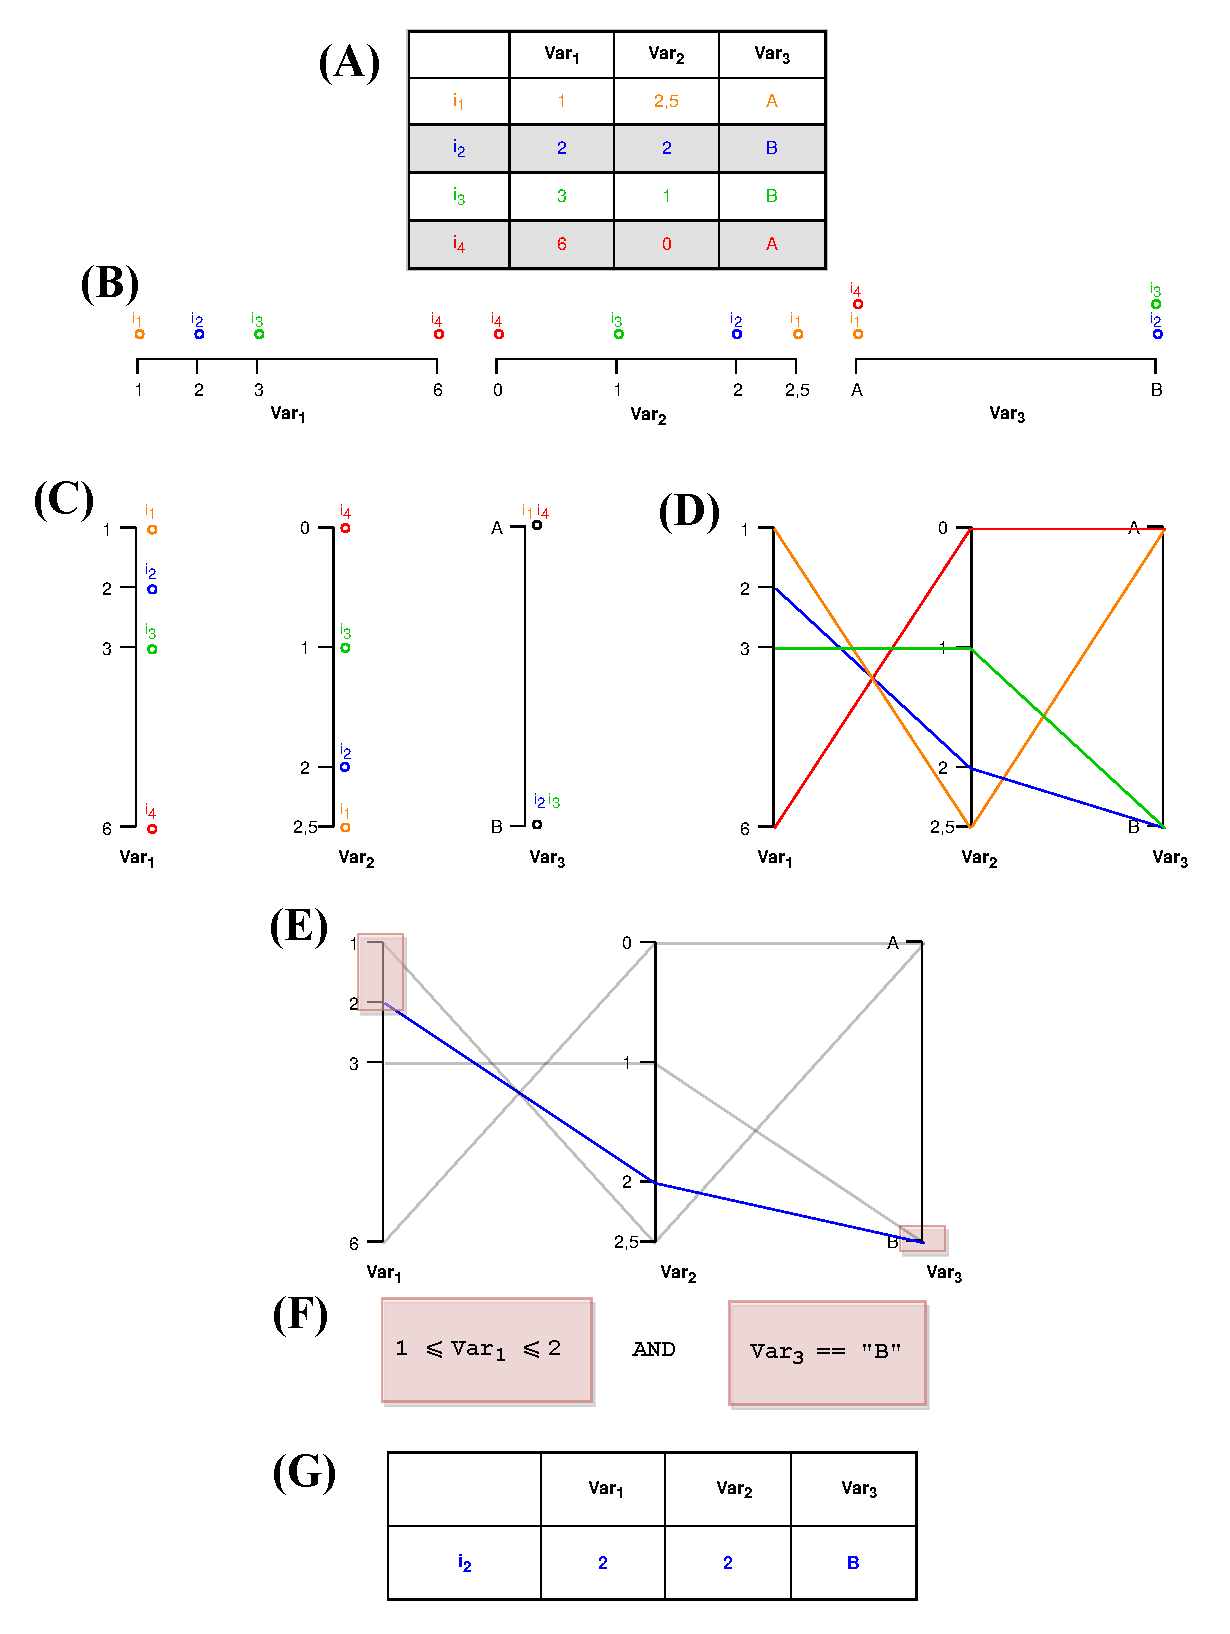
\includegraphics[width=\linewidth]{img/ParCoords_Brush.pdf}
			\caption{Démarche de construction d'un graphique en coordonnées parallèles (\textbf{A}--\textbf{D}) et sélection par \textit{brushing} (\textbf{E}--\textbf{G}).}
			\label{fig:schema_parcoords}
		\end{figure}

	\end{encadre}



	De plus, en matière d'interaction, on utilise fréquemment les graphiques en coordonnées parallèles en vue de filtrage, le plus souvent par des actions de \textit{brushing} (\og brossage\fg{}, c'est-à-dire sélection graphique d'une zone en dessinant son étendue à la souris -- cf. \cref{enc:parcoords}).
	Ce type de sélection se révèle en effet souvent plus efficace et intuitive qu'une sélection textuelle plus systématique :

	\begin{quotation}
		\og Filtering is an operation that removes signals from its input. A filter reduces the number of lines to be rendered. In this sense, dynamic querying [...] is a filter, if implemented with brushing [...], which reduces clutter by putting the filtered lines in focus using some highlighting mechanism. Combining simple brushes using logical operators [...] further allows the user to formulate rather complex queries that might even achieve faster and more accurate results using parallel coordinates than using a Structured Query Language (SQL) [...].\fg{}\\
		\mbox{}~ \hfill \cite[p. 13]{heinrich_state_2013}
	\end{quotation}

	Cette utilisation est aussi courante en géographie quantitative, et on la retrouve par exemple chez l'un des représentants de l'analyse spatiale des années 1990, Stewart Fotheringham, qui indique même l'usage du graphique en coordonnées parallèles en tant que filtre pour identifier des informations dans une autre dimension, spatiale ici : \og the data being displayed in parallel coordinates can be linked to a map and then brushed to highlight the locations of interesting lines displayed in \textit{m}-space on the parallel co-ordinates.\fg{} \autocite{fotheringham_trends_1999}.

	Appliqué aux données de SimFeodal, cette interface (\cref{fig:simvadb_dashboard}) se révèle particulièrement efficace pour sélectionner les configurations de paramètres à explorer.
	Ainsi, en \og brossant \fg{} quelques filtres manuellement (\cref{fig:simvadb_dashboard} - \textbf{A}), on arrive rapidement à isoler une expérience spécifique.

	\begin{figure}[H]
		\captionsetup{width=\linewidth}
		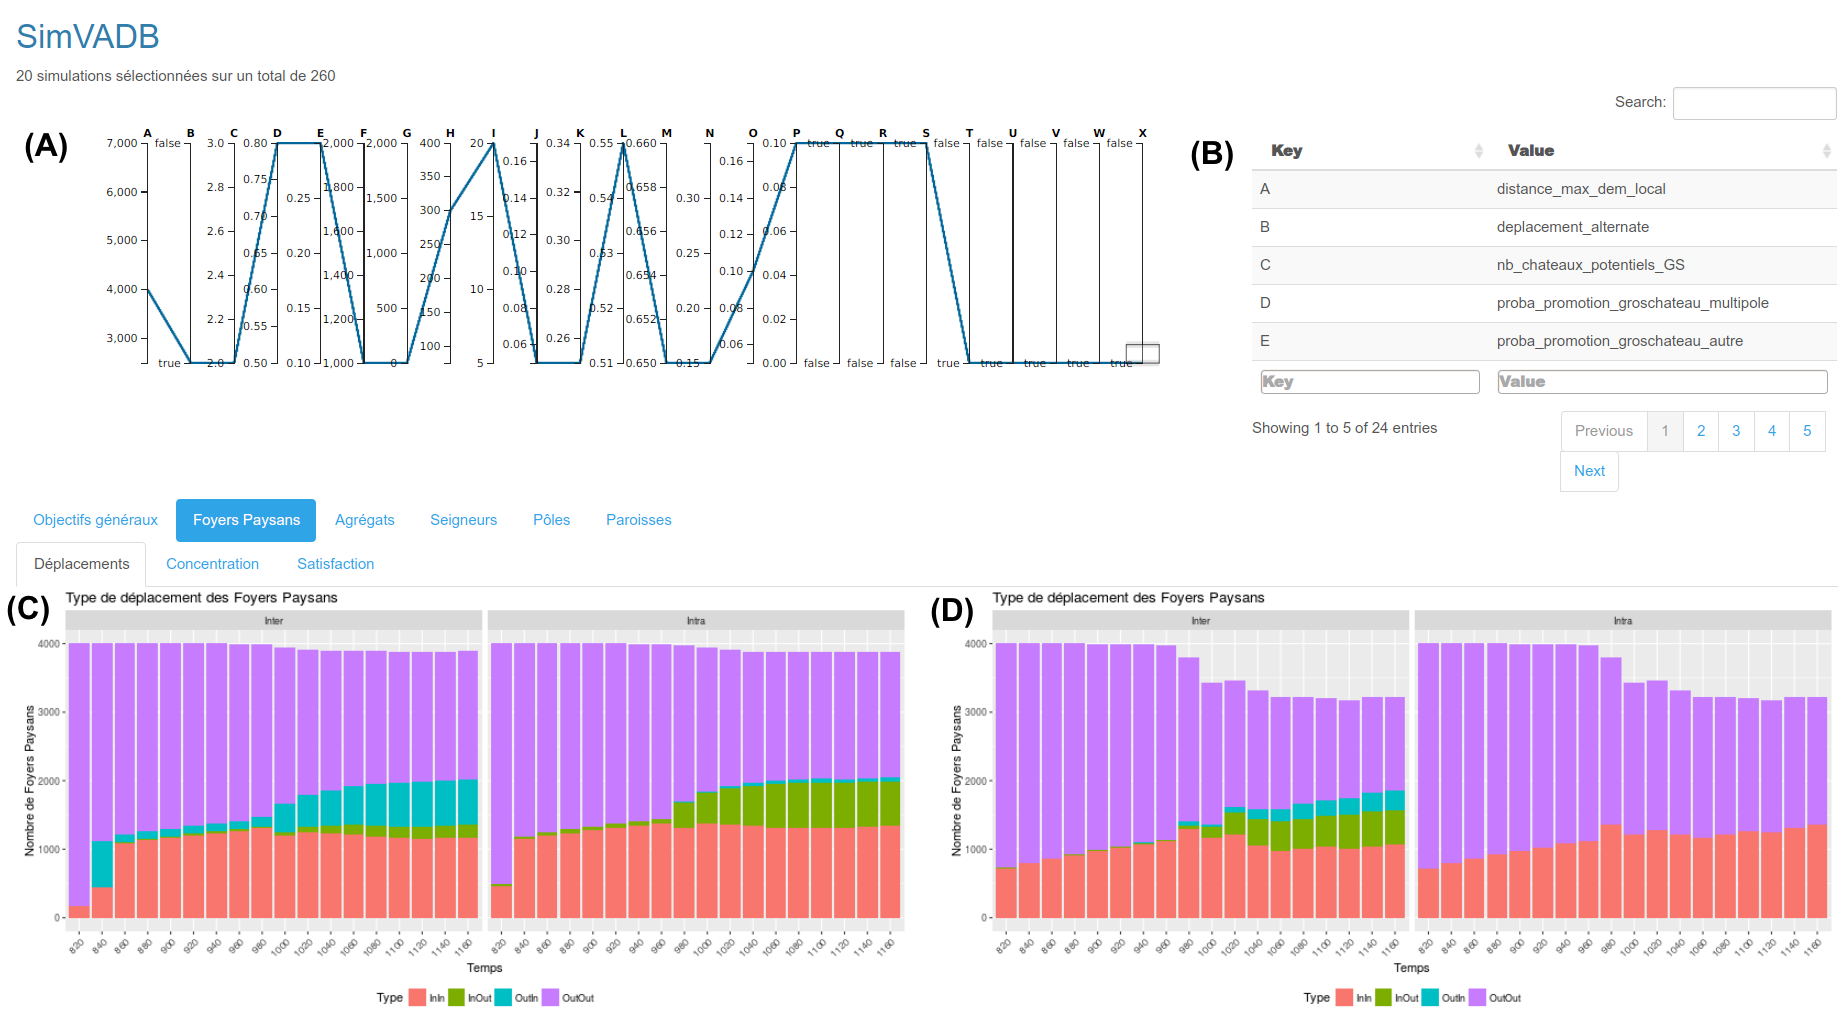
\includegraphics[width=\linewidth]{img/SimVADB_Dashboard2_annote.png}
		\caption{SimVADB (Simulation Visual Analysis DashBoard), un \textit{dashboard} d'exploration visuelle des indicateurs de sortie de simulation de SimFeodal.\\
		La sélection des simulations à explorer se fait dans le graphique en coordonnées parallèles (\textbf{A}), en \og brossant\fg{} des filtres graphiques sur les \og dimensions\fg{} du graphique, dimensions dont les intitulés sont explicités dans le tableau \textbf{B}.
		Les graphiques \textbf{C} et \textbf{D} indiquent l'évolution des types de déplacements des foyers paysans au cours des simulations.\\
		- Le graphique \textbf{C} représente, pour cet indicateur, une moyenne de l'ensemble des simulations intégrées dans la base de données (260 ici), recouvrant donc plusieurs valeurs de paramètres.\\
		- Le graphique \textbf{D} représente cet indicateur calculé depuis un sous-ensemble de 20 simulations (donc une expérience composée de 20 réplications), pour lesquelles le paramètre \og \texttt{X} \fg{}(\hl{Retrouver nom de ce paramètre}) vaut \texttt{true}.}
		\label{fig:simvadb_dashboard}
	\end{figure}

	Afin de permettre aux utilisateurs de remarquer les particularités des simulations explorées, nous avons choisi de mettre en emphase les différences entre la tendance générale des indicateurs, en calculant des moyennes de l'ensemble des simulations (\cref{fig:simvadb_dashboard} - \textbf{C}), et les valeurs spécifiques des indicateurs de l'expérience choisie (\cref{fig:simvadb_dashboard} - \textbf{D}).
	Cela permet, visuellement, d'être en mesure d'évaluer les sorties de simulation d'une expérience tout en ayant un référentiel visible.
	Les différentes expériences produisent des résultats sensiblement similaires\footnote{
		Si chaque expérience, et chaque réplication, produisent des résultats uniques, le choix d'une évaluation par des indicateurs visuels peut prêter à confusion si l'on n'a pas de repère précis.
		Les critères attendus, présentés dans \hl{le chapitre 3} sont ainsi assez précis pour départager une simulation très éloignée des attentes et une autre simulation plus conforme.
		Pour autant, par exemple quand les valeurs de paramètres varient faiblement, les résultats produits peuvent être assez similaires dans les grandes tendances qu'ils font ressortir.

	}, et on ne peut alors plus les comprendre sans les confronter à d'autres résultats similaires.
	Le choix d'une agrégation de l'ensemble des simulations effectuées est discutable, en ce qu'on aurait par exemple pu plutôt isoler des simulations \og de référence \fg{} afin de diminuer l'effet \og d'aplatissement \fg{} engendré par l'agrégation de résultats nombreux et hétérogènes.
	Toutefois, la variabilité des résultats étant encore assez restreinte, au moment de la création et de l'utilisation de SimVADB, ce référentiel agrégé permettait déjà une compréhension plus fine des sorties de simulations, en particulier dans l'analyse de l'impact de variations fines de valeurs de paramètres.

	\subsection{Explorer en comparant : SimEDB}\label{subsec:explorer-simedb}

	Après le travail de paramétrage grossier qui a permis de stabiliser les mécanismes, le paramétrage de SimFeodal est entré dans une phase plus fine, visant à mieux calibrer le modèle à l'aide de variations de valeurs de paramètres de granularité inférieures.

	Dans ce cadre, par exemple en faisant varier le nombre de foyers paysans de $4000$ à $4200$ ($5\%$ de variation), les résultats du modèle changent peu :  de faibles variations de valeurs de paramètres entraînent le plus souvent de faibles variations dans les indicateurs de sorties observés\footnote{
	On peut de plus noter que, les variations n'étant pas linéaires, les répercussions d'un changement de valeur de paramètre peuvent être très différentes de l'ordre de grandeur de ce changement de valeur. Par exemple, pour ces $5\%$ de variation dans le nombre de foyers paysans, la majorité des indicateurs variera de moins de $1\%$.
	}.

	En vue d'évaluer les simulations, et donc de les différencier les unes des autres à l'aune des indicateurs générés, la comparaison d'une expérience spécifique avec un référentiel constitué de toutes les expériences précédentes ne permet plus de mener ce travail de comparaison fine : par rapport à une référentiel unique, soit-il constitué d'une agrégation de simulations ou même d'une version \og de base\fg{} du modèle (par exemple les versions principales identifiées dans le \hl{chapitre 4}), les variations sont trop fines pour être distinguables les unes des autres.

	Pour pouvoir correctement évaluer les apports d'un nouveau jeu de valeurs de paramètres, et donc, dans une démarche itérative, pouvoir différencier deux expériences successives, il est donc nécessaire d'être en mesure de comparer directement les expériences les unes avec les autres.
	Il est donc indispensable de ne plus mener une comparaison visuelle entre un référentiel commun et une expérience spécifique, mais bien de baser l'évaluation sur la comparaison entre cette expérience spécifique et une autre expérience, tout aussi spécifique.

	D'un point de vue méthodologique, cela requiert de pouvoir afficher conjointement les indicateurs de sorties de deux expériences isolées de la masse des simulations.

	La sélection d'une expérience via l'usage de \textit{brushing} sur un graphique en coordonnées parallèles des valeurs de paramètres ayant montré son efficacité, il a été choisi d'étendre ce principe d'interactivité au choix du référentiel, c'est-à-dire de baser l'évaluation non plus sur la sélection d'une expérience spécifique, mais de deux expériences spécifiques.

	\clearpage
	\begin{figure}[H]
		\centering
		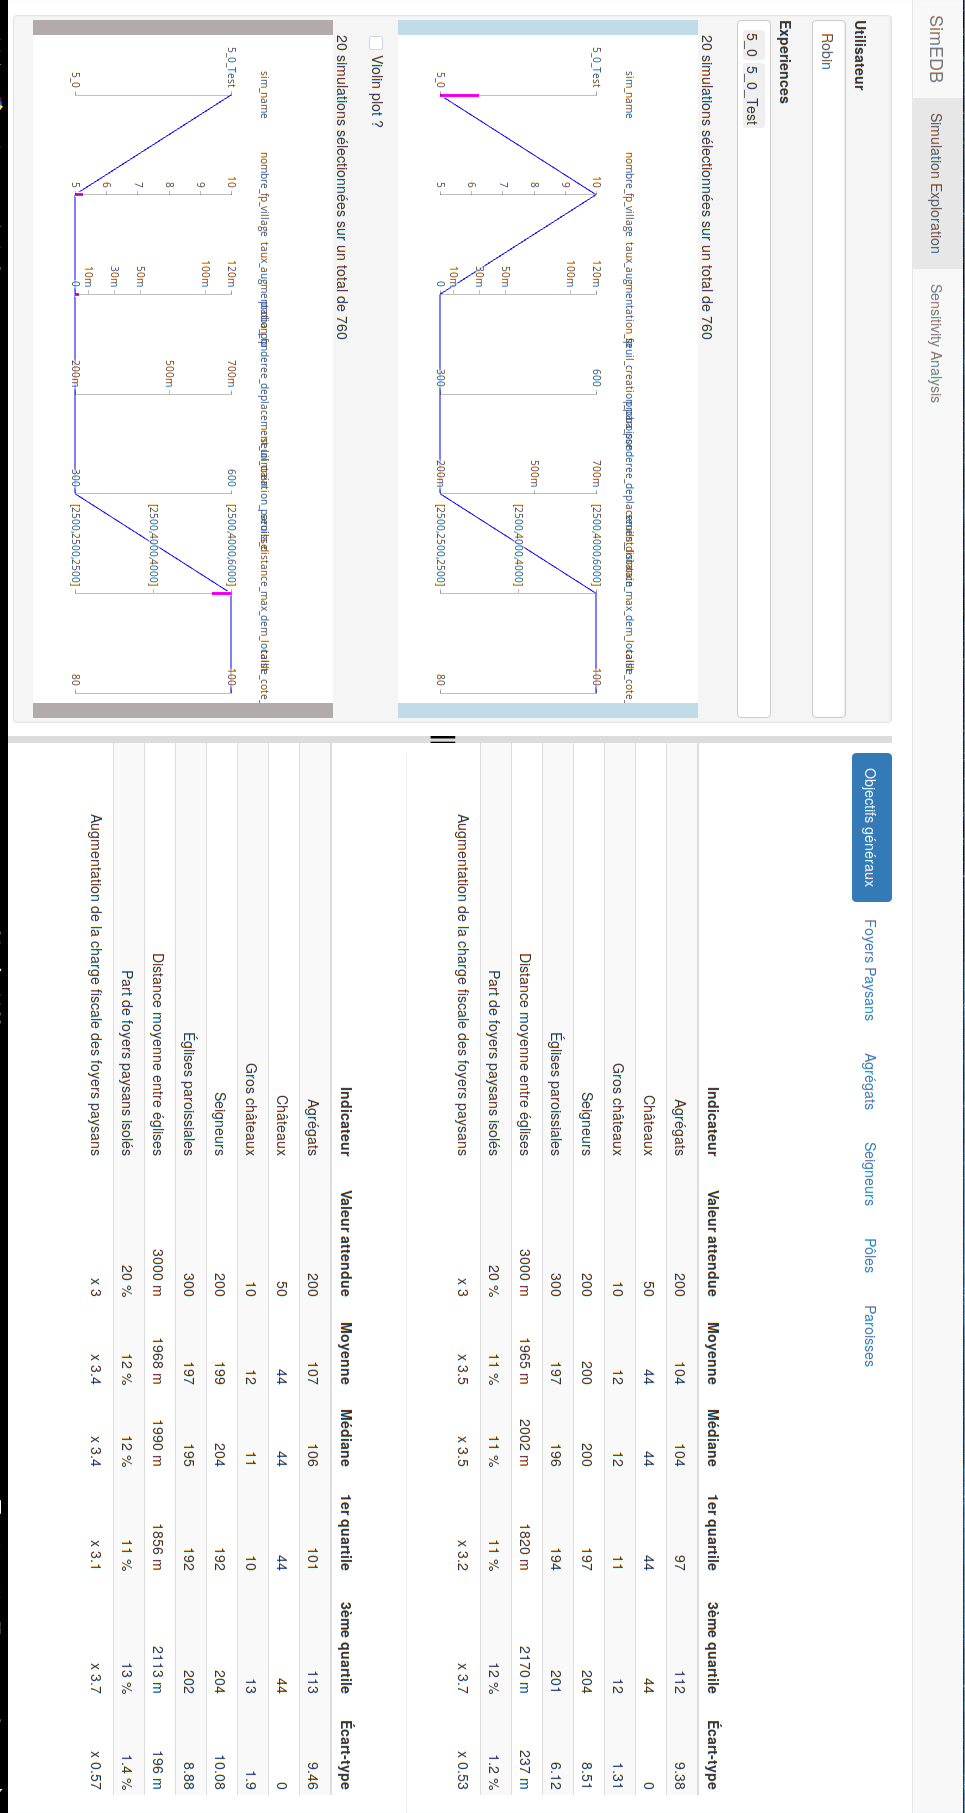
\includegraphics[width=.94\linewidth]{img/SimEDB_nombreFP_villages_rotate.png}
		\caption{SimEDB }
		\label{fig:simedb_villages}
	\end{figure}
\clearpage

	Dans cette version remaniée de la plate-forme d'exploration, renommée pour l'occasion SimEDB\label{par:introduction-nom-simedb} (\textbf{Sim}Feodal \textbf{E}xploration \textbf{D}ash\textbf{B}oard)\footnote{\label{ftn:origine-simedb}
		La plate-forme d'exploration SimVADB (SimFeodal Visual Analysis Dashboard) a été renommée SimEDB ([...] Exploration Dashboard) par soucis de simplicité, le terme \og Exploration\fg{} nous semblant plus compréhensible et explicite que celui de Visual Analysis. Cela permet de plus une cohérence sémantique entre plusieurs productions de l'auteur -- TimeLineEDB - \autocite{cura_timelineedb_2017}; RoadTrafficEDB et CitiBikeEDB - \autocite{cura_making_2017} --, inscrivant cette plate-forme d'exploration de données issues de simulation dans une \og famille \fg{} d'outils d'exploration de données spatio-temporelles.
	}, l'accent est donc mis sur la comparaison de deux ensembles de résultats, chacun répondant à une sélection propre.
	En superposant les graphiques et tableaux des indicateurs, la comparaison visuelle est facilitée.
	On peut alors aussi bien comparer deux variations fines d'un mécanisme -- en sélectionnant par exemple une unique différence dans les valeurs de paramètres (par exemple le nombre de foyers paysans présents à l'initialisation du modèle dans les villages (\cref{fig:simedb_villages}))) --, ou encore comparer les différences entre une version stable et les expériences en découlant -- en sélectionnant, par exemple dans la partie supérieure, une version que l'on estime suffisamment aboutie pour constituer un référentiel, et dans la partie inférieure, une série d'expériences issues de ce référentiel et qui font varier plusieurs paramètres.


	\paragraph*{}
	Nous reviendrons plus précisément et longuement sur la description de SimEDB dans les parties suivantes (\cref{sec:SimEDB}, p. \pageref{sec:SimEDB}), mais après en avoir décrit les étapes de construction et les besoins auxquelles ces évolutions répondaient, il est maintenant nécessaire de revenir sur les données manipulées par cette plate-forme d'exploration.
	Le type, la structure et la masse de ces données (\cref{sec:sorties-simfeodal}) sont en effet indissociables des choix méthodologiques effectués pour SimEDB.
	Il est donc important de présenter les choix et contraintes de ces données avant d'entrer dans une description approfondie de la plate-forme.

\clearpage
\section{Organiser les données}\label{sec:organiser-donnees}

On a vu dans la première partie de ce chapitre (\cref{sec:sorties-simfeodal}) que les données produites par SimFeodal étaient nombreuses, diverses et massives.
Contrairement à des modèles de simulations plus \og KISS \fg{}, par exemple les \og modèles-jouets\fg{} courants en Sciences Humaines et Sociales (\hl{ref Schelling/Sakoda, SugarScape, Prey-Predator, }), SimFeodal fait ainsi interagir de nombreux types d'agents, chacun doté de sorties spécifiques. Ces modèles sont le plus souvent évalués \og en direct\fg{}, les indicateurs présents dans l'interface des plate-forme de simulations suffisant à leur compréhension.
La démarche suivie pour l'évaluation de SimFeodal repose sur des indicateurs visuels, qui doivent être examinés \textit{a posteriori} de leur production (\cref{subsec:observation-a-posteriori}), et l'évaluation du modèle ne peut être réalisée qu'en s'appuyant sur une part importante de ces sorties.

Dans les modèles plus complexes utilisés en géographie (\hl{SimPop, MobiSim, SimPopLocal, MARIUS}), les données peuvent être plus massives (que ce soit intrinsèque au modèle (MobiSim) ou à sa méthode d'exploration (SimPopLocal)), mais leur structuration, souvent mono-agent, reste simple.

Pour SimFeodal, où les indicateurs s'appuient parfois sur des requêtes croisant plusieurs types d'agents, la question de la structuration de ces données revêt une importance cruciale.
Sans structuration adéquate, l'acquisition, l'archivage, l'interrogation ou encore la sauvegarde des données générées par le modèle ne peuvent être garantis, et encore moins de manière efficace.

Le choix d'une méthode d'organisation des données en sortie de simulations ne relève donc pas ici d'une quelconque coquetterie technique, mais, au contraire, conditionne et contraint fortement aussi bien les modalités de création des indicateurs que les possibilités de la plate-forme d'exploration de les afficher de manière interactive.

	\subsection{Assurer la capacité d'interrogation des données}\label{subsec:capacite-interrogation}

	Avant de se soucier du \og schéma\fg{} de la base de données\footnote{
		On utilise souvent le terme de \og schéma\fg{} pour désigner la version implémentée, dans un SGBD spécifique, du Modèle Conceptuel de Données (MCD). Contrairement au MCD, qui donne une version conceptuelle et générique d'une base de données, le schéma est donc tributaire du SGBD dans lequel il est intégré.
	}, du choix du Système de Gestion de Base de Données (SGBD), ou encore des performances de ce dernier, il convient de se fixer sur la manière dont on souhaite entreposer les données.

	De la myriade de fichiers issus de tableurs organisés dans une multitude de dossiers spécifiques à l'entrepôt de données décentralisé orienté documents, en passant par les traditionnelles bases de données relationnelles, les possibilités de stockage et d'organisation des données issues de simulations sont ainsi innombrables.

	Qui plus est, dans le but de générer et d'afficher des indicateurs de sorties de simulation \og à la volée \fg{}, la méthode d'interrogation (ou de \og requêtage \fg{}) des données stockées est un choix majeur, qui doit à ce titre précéder les autres.

	Dans le cadre des données issues de SimFeodal, en vue de leur mobilisation dans SimEDB, nous avons ainsi eu à sélectionner quelques SGBD candidats parmi foule de solution possibles.
	Afin de guider ce choix, trois critères ont été définies, et forment, selon une hiérarchie propre à leur ordre, un ensemble de filtre ayant permis la réduction des SGBD possibles à un nombre appréhendable.
	Ces critères, dont l'énonciation guidera cette partie, sont ainsi (1) l'universalité, ou \og agnosticité\fg{}, des SGBD aux outils de requête ; (2) la pérennité et stabilité des solutions disponibles et (3) les performances des SGBD considérés.

		\subsubsection{Interroger de manière universelle et indépendante}

		Lors de la conception d'un outil faisant appel à des données, qui plus est massives, il convient de se positionner tôt sur la manière d'interroger ces données.
		Par interrogation, on entend ici, comme souvent dans le domaine des bases de données, la manière de faire appel, concrètement, aux données, pour en tirer les sous-ensembles, agrégations et autres résultats synthétiques résultant du traitement des données brutes.
		Si l'on considère des données stockées dans un tableur, alors les \og formules \fg{}, les tableaux croisés dynamiques ou encore les graphiques issus du tableur sont des interrogations des données, qui s'expriment dans ce cas via un ensemble de langages, écrits -- les formules, qui font appel à des fonctions spécifiques des tableurs -- ou visuels -- les tableaux croisés dynamiques, construits en faisant glisser des intitulés de colonnes dans un tableau.

			\paragraph*{Stockage distribué ou centralisé}\label{par:stockage-centralise}
			Avant même de s'intéresser aux spécificités de ces langages, un premier choix réside dans le mode de stockage des données qui doivent être mis à disposition d'une plate-forme.
			Doit-on laisser l'utilisateur intégrer lui-même les données, et ainsi, en faire un stockage \og distribué \fg{}, dans le sens où chaque utilisateur de l'application possèderait physiquement une copie locale des données ?
			Ou, au contraire, les données doivent-elles être centralisées, c'est-à-dire enregistrées en une seule copie à laquelle les utilisateurs accèderaient à distance ?
			Pour reprendre l'exemple des tableurs, doit-on privilégier une solution locale -- chacun ayant une copie du fichier tableur et menant ses propres modifications dessus -- ou une approche de type centralisée, par exemple en privilégiant des tableurs collaboratifs en ligne (\textit{Google Docs/Sheets} par exemple) ?

			Habituellement, c'est-à-dire dans une grande majorité d'applications, les données sont stockées localement : cela permet, en particulier, de ne pas dépendre d'une connexion internet pour interroger des données qui seraient hébergées sur internet.
			Dans le cas de SimFeodal, cette solution est rendue difficile, sinon impossible, par la masse de données en sortie de simulations.
			Si chaque utilisateur de SimEDB devait posséder une copie des données, voir plusieurs en cas d'utilisations depuis différents ordinateurs, cela occuperait plusieurs gigaoctets de données à chaque fois.
			De plus, en cas de mise à jour des données, c'est-à-dire d'insertions de nouvelles sorties de simulations, il faudrait distribuer à nouveau l'ensemble du jeu de données, à chaque fois.

			Pour ces raisons, nous avons fait le choix d'un stockage centralisé, sous forme d'une architecture \og client-serveur\fg{}, hébergé sur un serveur internet dédié, ce qui permet à la plate-forme de travailler à chaque fois sur les données les plus à jour, réduit la taille du stockage physique associé, et dispense d'une configuration sur chaque poste utilisateur :
			si le lien entre l'application et les données fonctionne correctement pour un utilisateur, il fonctionnera à l'identique pour tous les autres.
			Ce choix présente un dernier avantage, non négligeable :
			en stockant les données en un seul lieu, c'est-à-dire sur un serveur informatique, on peut faire en sorte de rendre ce serveur aussi performant que possible, et accélérer ainsi l'interrogation des données pour tous les utilisateurs.

			\paragraph*{Interrogation spécifique ou générique}\label{par:interrogation-generique}

			De nombreuses solutions intégrées de gestion de données proposent leurs propres modes d'interaction avec les données, c'est-à-dire un langage spécifique permettant d'interroger les données contenues dans le système\footnote{
				Souvent, cette interrogation se fait par appel à des \textit{API} (\textit{Application Programming Interface}, ou Interface de Programmation Applicative en français) propres aux plate-formes, demandant donc un langage de requête spécifique.
			}.
			Au contraire, les SGBD les plus classiques s'appuient plutôt sur des langages de requêtes aussi standardisés que possibles, afin de faciliter l'adoption de leur propre solution à des utilisateurs d'autres plate-formes.
			La spécificité présente l'avantage de langages plus adaptés aux données manipulées, et donc souvent plus intuitifs dans l'interrogation des spécificités des données.
			De plus, la spécificité permet aussi une optimisation des requêtes, et est donc souvent plus performante que les solutions plus génériques.

			Dans le cas des données de SimFeodal, nous avons préféré privilégier une approche plus générique, faisant appel à des solutions de SGBD plus standardisées.
			La raison tient principalement à une volonté de généricité du stockage des données : au cours des différentes étapes de construction de SimFeodal, les besoins en matières d'interrogation des données ont évolué.
			Cette évolution était prévisible et prévue, et nous avons donc choisi dès le départ d'adopter uniquement des solutions modulaires, garantissant une évolutivité facilitée de la base de données, aussi bien regardant sa structure (enregistrement de nouvelles variables ou de nouveaux agents du modèle) que son contenu (massification des données en sortie au fur et à mesure de l'exploration du modèle).

			De plus, dans la perspective de ce travail de thèse, où l'on cherche à rendre autant les productions aussi reproductibles et génériques que possible, il était indispensable de disposer d'un SGBD aussi standard que possible pour en faciliter l'adoption et l'adaptation à d'autres modèles de simulations par exemple.

			\paragraph*{SQL ou NoSQL}\label{par:sql-nosql}

			Même une fois arrêté sur le choix de ne faire appel qu'à des outils standards pour stocker les données, le nombre de solutions disponibles demeure très important.
			Afin de réduire ce nombre, on peut déjà choisir les grands types de SGBD auxquels faire appel.
			Les SGBD sont ainsi souvent classés selon les grands traits de la méthode dont ils organisent les données.
			Les deux grands types\footnote{
				Il en existe d'autres, comme les SGBD orientés objets (quasiment disparus aujourd'hui), orientés graphes (Neo4j\ldots), les SGBD pensés pour le stockage et l'interrogation d'ontologies (\textit{Triplestores RDF}, interrogeables en langage SPARQL) ou encore les nouveaux SGBD de type \og NewSQL \fg{} (Apache Ignite, CockRoachDB\ldots) pensés pour une parallélisation massive des données. Ces types de SGBD ne correspondent toutefois pas du tout aux besoins identifiés pour SimEDB/SimFeodal, et sont en général dédiés à des problèmes et marchés de niches. Nous ne les décrirons donc pas plus en détail ici.
			} sont les SGBD \og relationnels\fg{} et les SGBD \og NoSQL\fg{}.
			Si la distinction est sujette à de très nombreux débats, souvent virulents
			\footnote{
				À l'instar des violentes querelles qui agitent régulièrement les informaticiens : Vim vs Emacs, Programmation Orientée-Objet vs Programmation Fonctionnelle, R vs Python\ldots
			}
			, on se contentera ici de définir les SGBD relationnels comme les SGBD, les plus fréquemment utilisés, où l'information est stockée dans des tables composées de champs -- les colonnes, correspondant aux variables -- et de lignes -- les entités décrites par les variables.
			Le format des données est donc rectangulaire et n'accepte pas, comme dans un tableau statistique, que les entités possèdent un nombre de variables différent, ou encore des types de valeurs différents de celles des autres entités (une même colonne ne peut donc contenir conjointement un nombre et un texte dans des lignes différentes).
			On nomme ces bases de données relationnelles via la manière qu'elles ont de faire communiquer des éléments hétérogènes, et donc contenus dans des tables différentes : si les tables ont une colonne en commun, on pourra alors effectuer une opération de jointure permettant de mettre en commun les informations de ces tables dans une unique table résultante.

			A l'inverse, les SGBD NoSQL se définissent de manière opposée à ce mode de stockage\footnote{
				À l'origine, c'était le sens fort du nom \og NoSQL \fg{} : Non SQL, le SQL faisant ici références aux SGBD pré-existants, majoritairement relationnels, dont la mouvance NoSQL, portée par l'apparition des \og \textit{big data} \fg{} a voulu se distinguer.
				Sans entrer dans le détail, notons tout de mêmes que de nombreux SGBD NoSQL, qui traduisent désormais cet acronyme par \og Not only SQL\fg{}, sont maintenant relationnels, mais mettent en avant d'autres types d'approches.
			}, rompant par exemple la contrainte d'unicité de type des colonnes, ou de nombre identique de colonnes renseignées pour chaque entité. Pour simplifier le discours, on se contentera de caractériser les SGBD NoSQL comme des SGBD non relationnels.

			Les SGBD NoSQL ont, en général, de bien meilleures performances et une plus grande flexibilité que les SGBD relationnels.
			Dans le cas de SimEDB/SimFeodal, où l'on est confronté à des données massives, cela présente un avantage non négligeable.

			Toutefois, leur flexibilité est associée à une contrainte majeure en termes de généricité : alors que les SGBD relationnels partagent un langage d'interrogation commun, le SQL (\textit{Structured Query Language})\footnote{
			Ce langage d'interrogation est omniprésent dans l'interaction avec les SGBD, mais aussi, avec de légères variantes, au sein de nombreux logiciels reposant des sélections de données, par exemple les logiciels SIG qui se basent sur la syntaxe du SQL (le fameux triptyque \texttt{\textbf{SELECT} \ldots~\textbf{FROM} \ldots{} \textbf{WHERE} \ldots})
			}, les SGBD NoSQL font plus souvent appels à des langages spécifiques à chaque SGBD.

			Pour SimEDB, cela impliquerait une fort dépendance au SGBD choisi : en cas de changement de SGBD, toutes les requêtes seraient à reformuler dans le nouveau langage, parfois même selon des logiques extrêmement différentes les unes des autres (dérivés du SQL, interrogations via des objets JSON, via des langages de parcours de graphes\ldots{}) etc.

			Au contraire, avec les SGBD relationnels, le langage de requête étant commun, une fois le code d'interrogation généré, il est très aisé de changer de SGBD cible.
			Cela procure donc une forte évolutivité aux outils d'interrogation de données tels que SimEDB, les fournisseurs de données étant interchangeables, ce qui permet donc d'en changer au fur et à mesure de l'apparition de nouveaux besoins.

			En raison de la généricité de ces solutions relationnelles, qui vient s'ancrer dans la recherche de reproductibilité et de généricité de notre démarche d'ensemble, nous avons donc choisi de faire reposer le stockage et l'interrogation des données sur des SGBD relationnels. Cette décision s'est montrée d'autant plus heureuse que, au cours de la construction et de l'évolution de SimEDB, le SGBD choisi pour héberger les données a changé plusieurs fois, sans demander de ré-adaptation, sinon minimes, des codes permettant leur interrogation en vue de produire les indicateurs de sortie depuis les données brutes en sortie de SimFeodal.


			\paragraph*{Entrepôts de données et interrogation directe}\label{par:interrogation-directe}

			En parallèle des SGBD, des solutions intermédiaires existent et visent à s'abstraire des SGBD en eux-mêmes pour mener les requêtes.
			Ces solutions, que l'on nomme Entrepôts de Données (\textit{Data Warehouses}), se comportent comme une surcouche faisant l'interface entre un ou plusieurs SGBD et la requête émise par le client final.

			Les entrepôts de données sont en particulier utilisés afin d'agréger des données provenant de différentes sources, que ce soient plusieurs bases de données relationnelles ou encore des assemblages de bases de données NoSQL et de bases de données relationnelles.

			Dans ces organisations, les entrepôts de données jouent aussi bien le rôle d'agrégateurs de données que d'environnements de manipulation et de restructuration de données (on les nomme alors \og ETL\fg{} -- \textit{Extract-Transform-Load}).

			Le grand intérêt de ces outils d'interface est d'abstraire la complexité de chacune des bases de données manipulées en générant une interface d'interrogation unique et générique, souvent performante grâce à des optimisations spécifiques (pré-calcul des requêtes possibles par exemple).

			Dans le domaine de la visualisation interactive de données, ces outils sont beaucoup utilisés, en particulier dans le monde de l'informatique décisionnelle.
			Ils se révèlent en effet extrêmement utiles quand les données sources ne peuvent être modifiées (par exemple quand elles sont issues de chaînes de collecte complexes, ou encore quand leur volumétrie et leur débit est important), puisqu'ils permettent de constituer une surcouche rendant l'interrogation et la visualisation de ces données accessibles à des analystes non spécialistes de la manipulation de données.
			Toujours en informatique décisionnelle, il est courant de faire appel à des entrepôts de données d'un type spécifique, les \og traitements analytiques en lignes\fg{}, ou environnements OLAP (\textit{\textbf{O}n\textbf{L}ine \textbf{A}nalytical \textbf{P}rocessing}), qui permettent de structurer, par exemple sous formes de cubes de données, des sources de données hétérogènes présentant de nombreuses dimensions.

			Les environnements OLAP ont été utilisés, promus et adoptés dans le champs scientifique de la géomatique, en ce qu'ils permettent de mettre en place rapidement des environnements d'analyse visuelle de données multi-dimensionnelles spatiales et temporelles.
			Dans ce cadre, où ces outils sont appelés \og SOLAP\fg{} (\textit{Spatial OLAP}), les données spatiales s'intègrent extrêmement bien en raison de leur capacité à s'emboîter selon les échelles, ouvrant dès lors la voie à des analyses multi-échelles et multi-dimensionnelles complexes.

			Dans la communauté géomatique francophone, les solutions SOLAP sont bien représentées (par exemple autour de Sandro Bimonte et de son travail de visualisation de données spatiales environnementales,  \autocite{bimonte_integration_2007, bimonte_towards_2005, zaamoune_new_2013}), et sont couramment employées pour répondre à des questionnements méthodologiques proches de ceux développés dans cet ouvrage.
			En lien avec les besoins de performances identifiés plus haut, on notera que certaines solutions OLAP permettent aussi d'optimiser la vitesse d'interrogation de bases de données, et visent ainsi à garantir une réponse rapide pour des outils d'interrogation de données interactifs \autocite{zeng_iolap_2016}.

			Nous avons cependant choisi de ne pas faire usage de ces outils pour les mêmes raisons que pour les SGBD NoSQL : les avantages qu'ils présentent ne suffisent pas à contre-balancer les défauts en termes de généricité qu'ils introduisent. Pour profiter au mieux de ces environnements, il est en effet nécessaire de faire appel à un nouveau langage d'interrogation des données (le \og MDX\fg{}, de \og \textit{Multidimensional Expressions}\fg{}).
			Les différentes solutions OLAP/SOLAP, de plus, présentent les mêmes inconvénients que les SGBD NoSQL : chacune interagit de manière propre aux différents SGBD, et ces outils sont donc difficilement interchangeables.

			De la même manière, on se restreindra, parmi les SGBD relationnels interrogeables en SQL, à ceux qui disposent d'une méthode d'interrogation standard : si tous ces SGBD acceptent le SQL, certains demandent par exemple des protocoles spécifiques pour recevoir établir la connexion au SGBD, recevoir la requête et renvoyer les données correspondantes.
			Pour ce même choix \og d'agnosticité \fg{} de la plate-forme d'interrogation face à la solution de stockage choisie, on ne conservera que les SGBD acceptant les connexion standardisées (ODBC et JDBC).

			\paragraph*{SGBD et données spatiales}\label{par:sgbd-spatial}

			On a mentionné le fait que les entrepôts de données étaient fortement utilisés, en particulier dans la communauté géomatique, car très appropriés aux données spatiales.
			De prime abord, ce point peut paraître critique : jusque là, on s'est contenté de mentionner les capacités organisationnelles de SGBD, et non leur aptitude à manipuler des données spatiales.
			Ce point, dans les SGBD relationnels, constitue un filtre important : sur la centaine de solutions disponibles, seule une poignée est en mesure de stocker efficacement et d'interroger de l'information spatiale \footnote{
				Les données spatiales peuvent être stockées dans tous les SGBD si l'on attribue une représentation textuelle, en chaînes de caractères, par exemple en utilisant le format \textit{Well-Known Text} (WKT). Pour autant, ce format est lourd, inadapté à une indexation, et ne peut permettre à un SGBD de mener des requêtes spatiales directement depuis ces entités. Il est ainsi, par exemple, impossible de calculer le centroïde d'un polygone directement depuis une représentation WKT, alors que c'est aisé avec un stockage géométrique.
			}.

			Pourtant, au regard des indicateurs de sortie de simulation sur lesquels on s'appuie pour évaluer le comportement de SimFeodal, une grande majorité est non spatiale, en raison de la difficulté à agréger des données spatiales théoriques.
			La gestion de données spatiales ne constitue donc pas une absolue nécessité, contrairement aux points évoqués auparavant, mais peut toutefois se révéler avantageuse, ne serait-ce que pour permettre l'observation des configurations spatiales simulées, quand bien même celles-ci ne peuvent constituer qu'une approche idiographique, visant à exemplifier plus qu'à synthétiser.

			\paragraph*{}
			Pour héberger et organiser les données produites par SimFeodal, en vue de leur interrogation dans SimEDB, nous avons choisi de restreindre la myriade de solutions disponibles à des solutions centralisée (\nameref{par:stockage-centralise}), au sein de Systèmes de Gestion de Base de Données (SGBD) permettant une interrogation standardisée (\nameref{par:interrogation-generique}) via un langage de requête universel, le SQL (\nameref{par:sql-nosql}), envoyé directement aux SGBD sans passer par l'intermédiaire d'entrepôts de données, et au travers de connexion aussi standardisées que possible (\nameref{par:interrogation-directe}).
			Les SGBD répondant à ces critères sont les SGBD \og relationnels \fg{}, dont certains possèdent qui plus est une capacité intéressante à stocker et interroger des données spatiales (\nameref{par:sgbd-spatial}).

		\subsubsection{Interroger de manière robuste et efficace}\label{subsubsec:interroger-robuste-efficace}

		En dépit de l'accumulation de critères exposée précédemment, une quantité importante de SGBD demeurent en lice.
		Afin de les différencier, nous avons choisi d'ajouter des critères qui ne portent plus sur les grands types de SGBD, mais plutôt sur une différenciation des SGBD relationnels existants.
		Les critères ajoutés, la robustesse et la performance, ne sont pas des \og prétextes \fg{} à une objectivation d'un classement des SGBD, mais ont une importance prépondérante dans notre cas d'utilisation.

		\paragraph*{Robustesse des SGBD}
		Le premier critère est celui de la robustesse, c'est-à-dire, ici, de la capacité du SGBD à être interrogé de manière stable et pérenne dans le temps : une même requête sur les mêmes données doit systématiquement renvoyer le même résultat (stabilité), quelque soit la durée séparant ces requêtes (pérennité) : si la base de données n'est plus interrogeable quelques mois après sa configuration, ou qu'elle renvoi des résultats différents, alors elle ne peut constituer une solution crédible à l'exploration d'un modèle sur une période longue.

		\subparagraph{Stabilité}
		La stabilité des bases de données est principalement due à la manière de stocker l'information d'un point de vue informatique : quand l'information est stockée dans un unique fichier, ou dans plusieurs fichiers contenant l'information \og en clair\fg{}, donc sans mécanismes de réparation, il peut arriver qu'une base de données soit \og corrompue\fg{}.
		Par exemple, si l'on exécute une requête demandant un calcul complexe et long et que cette requête est interrompue en cours par faute d'un \textit{bug} ou d'une expiration de sessions (\textit{timeout}), il se peut que la base de données s'arrête dans un état muté -- avec une nouvelle table ajoutée pour moitié par exemple -- et ne soit donc plus intègre.
		C'est très fréquent pour les SGBD basés sur un unique fichier, ou encore stockés en mémoire vive (\og \textit{in-memory}\fg{}), puisque les nouvelles informations de la base de données y sont ajoutées au fur et à mesure, plutôt que d'être intégrées dans un fichier annexe que l'on pourrait réinitialiser en cas d'erreur.

		Avec la volumétrie des données produites par SimFeodal, les requêtes peuvent s'avérer très longues, et une erreur dans une requête peut fréquemment corrompre la base de données.
		En termes de stabilité, on se tournera donc plutôt vers des SGBD relationnels stables, basés sur une redondance des données et donc sur des stockages non-fichiers.

		\subparagraph{Pérennité}
		La pérennité des SGBD est un sujet proche, tenant aussi à la capacité à interroger les données contenues dans une base de données, mais cette fois-ci du point de vue de l'interrogation en elle-même plutôt de des données sur lesquelles elle s'applique :
		si le SQL est un langage standard\footnote{
		Dans les faits, on notera tout de même qu'il existe plusieurs normes successives, des \og révisions\fg{} du SQL, qui apportent chacune leur lot de subtilités dans l'usage du langage. Les SGBD interrogeables en SQL ne disposent donc pas toutes des mêmes fonctionnalités, selon la révision du SQL qu'elles respectent.
		}, les types de données intégrées varient cependant d'un SGBD à un autre (champs textuels ou d'entiers \og courts\fg{} par exemple).
		SQL étant un langage typé, selon la manière (bas niveau) dont sont intégrées les données, certaines requêtes identiques peuvent renvoyer des résultats différents selon les SGBD.
		Plus gênant, les normes implémentés peuvent varier d'une version à l'autre d'un SGBD : un SGBD relationnel qui respectait strictement la norme SQL pourrait évoluer pour supporter plus de fonctionnalités, par exemple en ajoutant des fonctions plus récentes (fenêtres glissantes, ajouts en masse etc.), et renverrait dès lors des résultats différents selon les versions.
		Pour les SGBD les plus employés, le nombre d'utilisateurs garanti une rétro-compatibilité des requêtes.
		Pour les SGBD de moindre envergure cependant, par exemple les plus performants et récents, issus de la recherche en informatique, cette rétro-compatibilité n'est pourtant pas du tout garantie.

		Comme souvent en matière d'infrastructure informatique, il est donc nécessaire de tenir compte d'un compromis entre l'ancienneté et la forte adoption de certains SGBD d'une part, et les facilités et gains de performances amenées par les plus récents d'autre part.

		Dans le cas des données de SimFeodal, en tenant compte de cet inévitable compromis, nous avons choisi de privilégier des SGBD reconnus, soient-ils anciens et fortement adoptés ou plus récents mais utilisés par des acteurs d'envergure\footnote{
			La liste des solutions envisagées, ensuite comparées à l'aube de leurs performances, est visible dans l'axe des ordonnées de la \cref{fig:db-benchmarks}.
		}.
		Ce faisant, on se coupe immanquablement de solutions extrêmement intéressantes et performantes\footnote{
			Par exemple BlinkDB \autocite{agarwal_blinkdb_2013}, qui permet de limiter une requête à un temps maximal d'exécution donné : quand la requête n'est pas complète, le SGBD renvoi une estimation du résultat, estimation qui gagne en précision quand on augmente la limite temporelle. Un SGBD de ce type serait extrêmement précieux en \textit{visual analytics}, mais la jeunesse de cet outil ainsi que sa nature de projet de recherche rendent incertain la continuité de son développement dans le temps. En 2018, le projet semble d'ailleurs abandonné depuis\ldots
		}, au prix d'une meilleure garantie de pérennité, et de robustesse en générale, des données de SimFeodal.

			\paragraph*{Performance des SGBD}

			Une fois que les solutions disponibles ont été discriminées par leur type, par leur interface avec les requêtes et par leur robustesse, la quantité de SGBD restant demeure de l'ordre de la dizaine.
			Pour choisir, parmi ceux-là, le SGBD qui sera le plus adapté aux besoins identifiés, il est donc nécessaire d'établir des critères plus précis et quantifiables.
			Dans le cas d'une application interactive, c'est-à-dire où le nombre de requêtes émises au cours d'une session d'utilisation peut être importante, les performances des SGBD constituent le critère principal.
			En tant que tel, il est difficile de juger des \og performances\fg{} d'un SGBD, c'est-à-dire qu'on entend en fait par là un vaste ensemble hétérogènes de propriétés.
			On peut par exemple juger les performances par le filtre de la mémoire occupée par le stockage d'une base de données, ou encore par le nombre de requêtes concurrentes que peut gérer un SGBD, ou encore par la capacité à paralléliser le stockage sur plusieurs serveurs.
			Dans notre cas, ces points sont assez peu significatifs : en dépit de la quantité de sorties, l'ordre de grandeur -- quelques gigaoctets de données -- reste largement entreposable sur un environnement classique, sans besoin de parallélisation.
			De la même manière, SimEDB est un environnement dédié à des utilisateurs experts, en petit nombre : les chercheurs travaillant autour de SimFeodal. La quantité de requêtes simultanées ne peut donc pas dépasser la dizaine, ce qui constitue une trivialité pour l'ensemble des SGBD relationnels classiques.

			On s'attachera donc à juger les performances en matière de rapidité des requêtes.
			Il ne s'agit pas ici de choisir un SGBD qui ferait gagner quelques millisecondes par rapport à un autre, mais plutôt de discriminer les SGBD présentant une durée de réponse trop importante pour notre usage.
			En effet, plus les données sont massives, plus le temps d'exécution d'une requête augmente.
			Si tous les SGBD présentent des vitesses acceptables et peu comparables sur des bases de données légères d'exemple, l'écart s'accroît considérablement à mesure que les données s'accumulent.
			La \cref{fig:db-benchmarks}\footnote{
			Dans cette figure, on compare la rapidité de différentes requêtes sur un jeu de données identique selon les SGBD. Ce jeu de données, composé de 100 Millions de lignes, présente une volumétrie comparable à celle des données issues de SimFeodal qui sont interrogées dans SimEDB.
			} montre les différences incontestables qui existent entre les SGBD étudiés. On peut y constater que l'écart est gigantesque, par exemple vis-à-vis du temps nécessaire à une jointure, entre les 4 secondes de MonetDB et les 300 secondes (5 minutes\ldots) de SQLite.
			Le choix d'un SGBD selon ses performances n'est donc pas, ici non plus, un choix mineur.

			\begin{figure}[H]
				\centering
				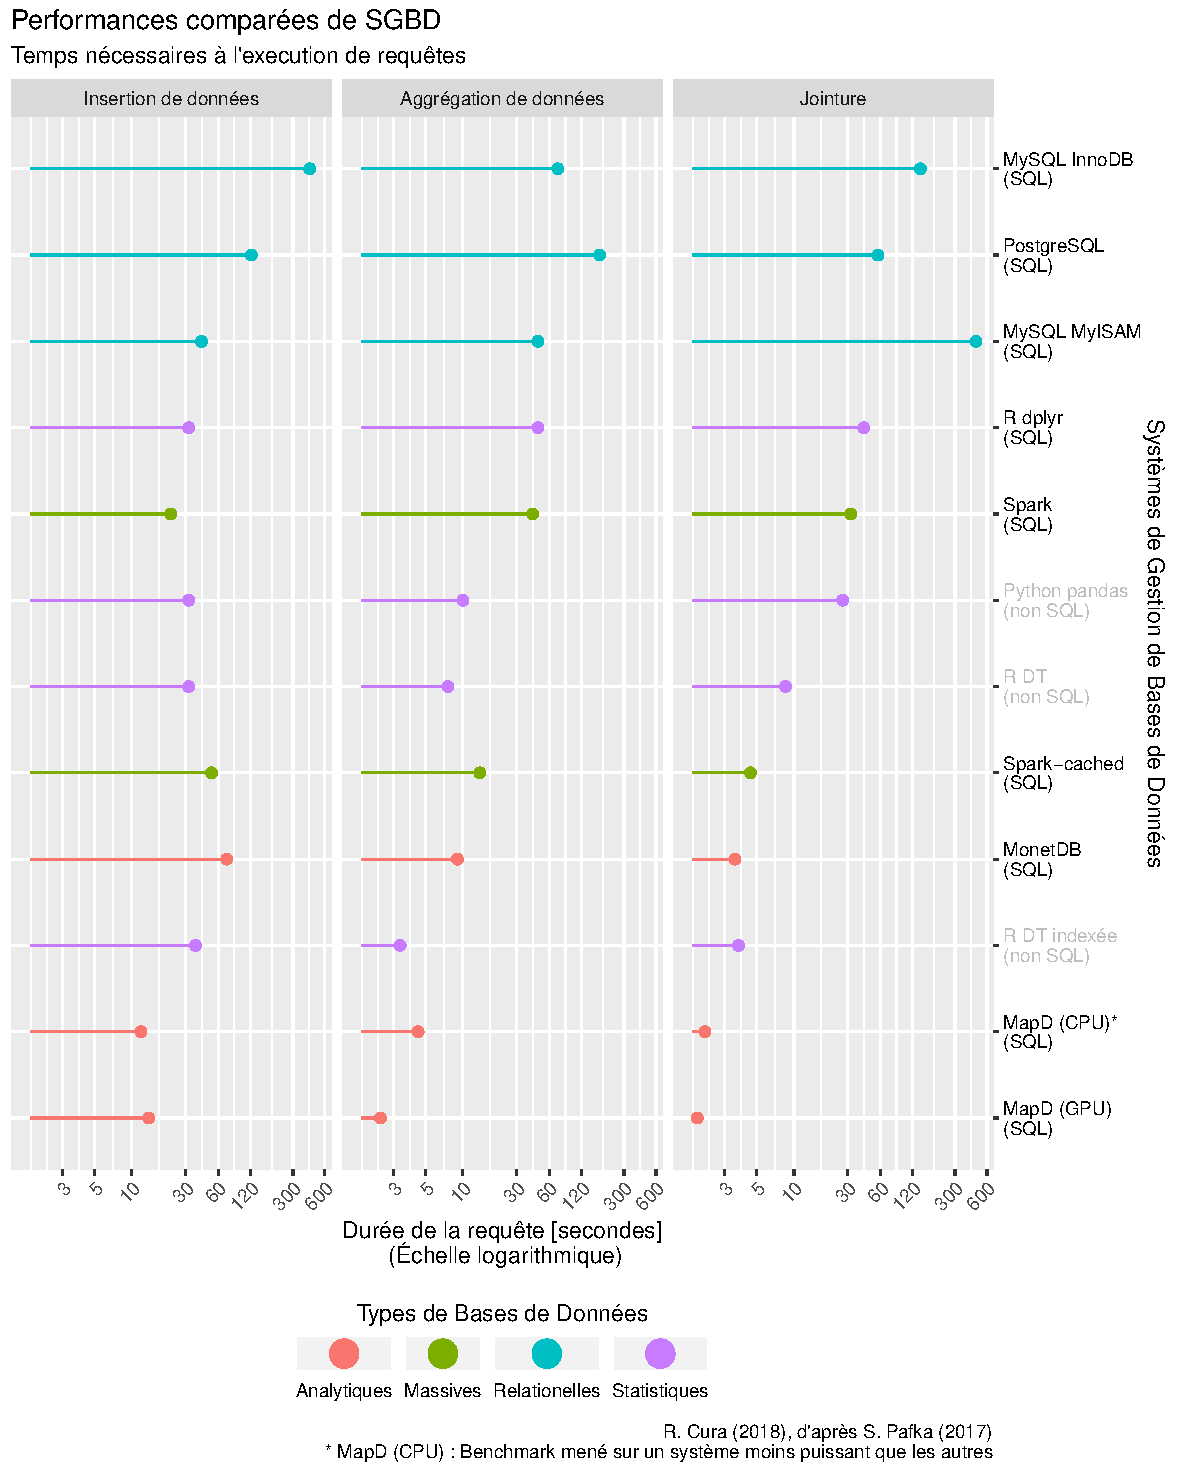
\includegraphics[width=\linewidth]{img/benchmark_results.pdf}
				\caption[Comparaison de la performance de différents SGBD sur un jeu de données test de 100 millions de lignes.]{Comparaison de la performance de différents SGBD sur un jeu de données test de 100 millions de lignes.\\
				Résultats extraits de \autocite{pafka_benchm-databases_2017} enrichis (SQLite, MapD CPU).\\
				Les \og types de Bases de Données\fg{} correspondent aux usages les plus fréquents des SGBD comparés :\\
				- Analytiques : SGBD optimisés pour les traitements de type agrégation, via une architecture orientée colonne plutôt qu'orientée ligne comme dans les SBGD Relationnels\\
				- Massives : SGBD pensés pour la gestion et l'interrogation de données massives (big data), permettant notamment une parallélisation des requêtes.\\
				- Statistiques : SGBD internes aux environnements de traitement de données statistiques, reposant sur une gestion en mémoire vive. Souvent intégrés d'office dans les environnements décrits (R, Python), ce sont les SGBD les plus simples à mettre en place et à manipuler.
			}
				\label{fig:db-benchmarks}
			\end{figure}


			\subparagraph{Performances en écriture et en lecture}

			La \cref{fig:db-benchmarks} affiche des résultats qui semblent globalement ordonnés (les quatre premiers SGBD sont par exemple quasiment toujours plus lents que les 2 derniers), mais fluctuent cependant à la marge selon les opérations demandées.
			La première colonne du graphique montre ainsi le temps nécessaire à l'insertion du jeu de données exemple (100 millions de lignes) dans le SGBD depuis un fichier CSV.
			Les deux colonnes suivants exposent le temps nécessaire au traitement d'une requête, donc à une interrogation des données une fois archivées dans les bases de données.
			On peut constater que le classement des SGBD varie à la marge, et en particulier entre les opération de lecture et d'insertion.
			Dans un environnement classique, la performance d'insertion de données est un facteur prépondérant : quand de nouvelles données sont ajoutées constamment, par exemple pour stocker des données issues de capteurs automatiques, l'insertion peut vite constituer le goulot d'étranglement de la solution.

			Pour SimFeodal, l'insertion n'est pas véritablement un enjeu : les données sont ajoutées par bloc, manuellement, une fois que des nouvelles simulations ont été exécutées.
			C'est donc au pire un acte quotidien, mais dans ce cas, que la requête demande 10 secondes (MapD) ou 10 minutes (MySQL InnoDB), cela n'a que peu d'impact.

			La première colonne donne donc une idée des performances, mais ne revêt pas un critère indispensable dans notre cas.

			Les deux colonnes suivantes, relatives à l'interrogation de données, se révèlent au contraire extrêmement importantes : à chaque action de l'utilisateur de SimEDB, une nouvelle requête est envoyée pour calculer un nouvel indicateur correspondant au jeu de données filtré manuellement (cf. \cref{subsec:explo-interactive}).
			À chaque affichage d'onglet, une nouvelle requête est donc émise et traitée. Même si tous les indicateurs ne sont pas systématiquement mobilisés -- et donc calculés -- (cf. \hl{chap 3}), cela signifie tout de même que pour chaque sélection, une bonne dizaine d'indicateurs seront observés, et donc, autant de requêtes.
			Avec un temps d'exécution de 60 secondes (PostgreSQL en \og jointure\fg{}), cela implique que chaque indicateur requiert une minute avant de s'afficher, et donc, une bonne dizaine de minutes ne serait-ce que pour charger les indicateurs, sans donc tenir compte de la durée nécessaire à leur analyse par l'utilisateur.
			Pour noircir le trait, notons de plus que les résultats communiqués dans la \cref{fig:db-benchmarks} correspondent à des requêtes exemples simples.
			Dans le cas de SimEDB, le calcul des indicateurs requiert des requêtes plus complexes, faisant appel à des agrégations et à des jointures en même temps, et les délais affichés dans ce \textit{benchmark} sont donc bien moindre que les durées éprouvées en conditions réelles au sein de SimEDB.

			\subparagraph{De l'intérêt de gagner quelques secondes}

			La \cref{fig:db-benchmarks} permet d'isoler un sous-ensemble de SGBD ayant, avec le jeu de données testé, des réponses inférieures à une dizaine de secondes.
			On pourrait se contenter de choisir le SGBD le plus complet parmi les 4 solutions identifiées (Spark avec cache, MonetDB ou les deux configurations de MapD).

			Pourtant, les conclusions d'un domaine parallèle se révèlent précieuses pour ne pas suivre ce raisonnement :
			dans le monde des sites internet, donc d'environnements dotés de multiples pages qu'un utilisateur consulte avant de passer à la suivante, de nombreuses études ont montré que la durée d'affichage d'une page jouait de manière considérable sur l'usage d'un site.
			Neil Patel, par exemple, relate une expérience vécue au sein du moteur de recherche Google  :

			\begin{quotation}
				\og
			Google did an interesting experiment with regard to load times. Google Vice President Marissa Mayer asked web surfers – would you rather see 10 or 30 results for your Google search? The users agreed that 30 results per page sounded like a good idea. So Google implemented it on some results pages.\\
			Then the shock came.\\
			Pages that displayed 30 results each had traffic to them drop an astounding 20\%. Google tested the loading difference between the 10 and 30 results pages and found that it was just \textbf{half of a second}. If half of a second made that much of a difference in how long users were willing to wait, how much of a difference could it make to your site if you carved a second or two off of load time?
				\fg{}\\
				\mbox{}~ \hfill  \autocite{patel_speed_2011}
			\end{quotation}

			Si l'environnement et les conditions décrites ne sont naturellement pas directement comparables avec celles de SimEDB, il demeure qu'une différence même faible dans un temps de chargement, ou, pour SimEDB, dans un temps d'affichage d'un indicateur de sortie, pourrait avoir des conséquences négatives pour l'utilisation de la plate-forme.

			Dans un cadre plus proche du notre, relatif au nombre de pages visitées en moyenne sur un site web (\cref{fig:page-abandon}), ce que l'on peut donc directement assimiler au nombre d'indicateurs consultés dans SimEDB, on peut aussi se rendre compte que quelques secondes de différence ont un impact là encore crucial dans l'utilisation qui sera faite d'un site.

			\begin{figure}[H]
				\centering
				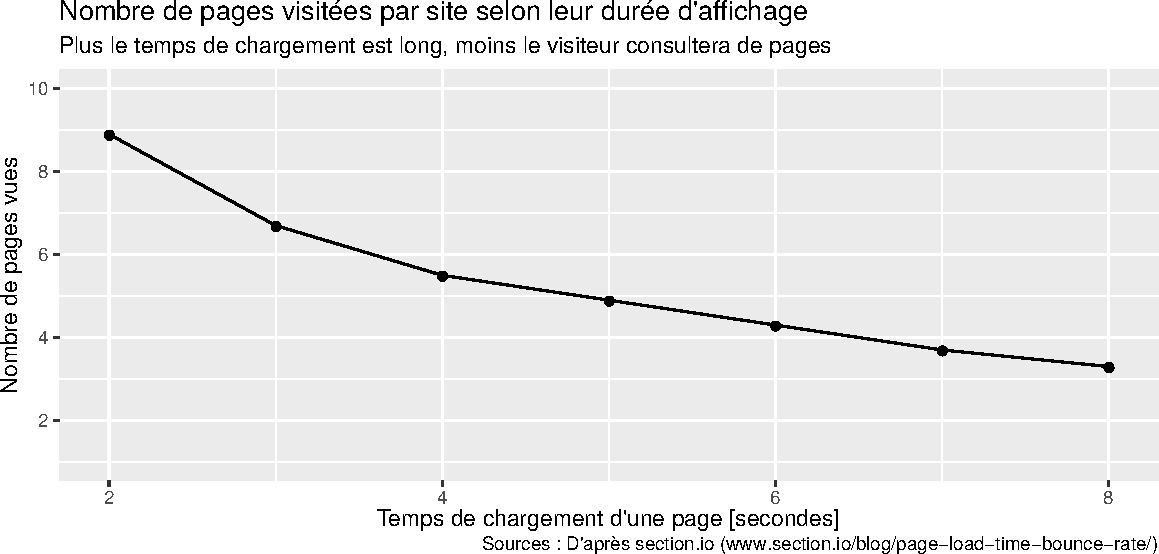
\includegraphics[width=\linewidth]{img/abandon_pages.pdf}
				\caption{Impact du temps de chargement des pages web sur le nombre de pages consultées au cours d'une session. D'après \cite{elliott_how_2017}.}
				\label{fig:page-abandon}
			\end{figure}

			On peut toutefois pondérer ces comparaisons et minimiser l'importance d'écarts de l'ordre de grandeur de la seconde.
			En effet, dans le cas de SimEDB, contrairement à celui d'un site web ou d'un moteur de recherche, l'utilisateur est captif : un thématicien souhaitant explorer les résultats de sur SimFeodal n'aura d'autre choix que de passer par SimEDB.
			De même, sachant que la plate-forme présente pour lui un intérêt professionnel, il sera bien pus patient que face à un quelconque site de courses en lignes.

			Dans le cadre d'environnements de type \textit{visual analysis}, il a été montré que les utilisateurs d'environnement d'exploration étaient toutefois fortement affectés par l'accroissement de délais.
			Zhicheng Liu et Jeffrey Heer \autocite{liu_effects_2014} montrent ainsi qu'en introduisant une latence supplémentaire de 500 ms dans une application interactive d'exploration de données spatio-temporelles, le nombre d'interactions chute fortement, quand bien certains utilisateurs de cette application ne remarquent même pas la différence de délai.

			\paragraph*{}

			Il ressort de cet ensemble successif de filtres que les solutions appropriées à l'organisation des données issues de SimFeodal sont assez peu nombreuses et diverses.
			Au regard des performances de chacun des SGBD, MapD \autocite{root_mapd_2016} présente l'avantage indéniable de la vitesse de traitement des requêtes, tout en étant compatible avec les standards de l'interrogation de données (langage de requête SQL, interfaçable via JDBC).
			Quand bien même nous ne disposons pas des infrastructures qui sont en mesure d'exprimer les meilleurs performances de ce SGBD\footnote{
				MapD est ainsi un SGBD optimisé pour l'analyse sur processeurs graphiques (les GPU), présents dans les cartes graphiques modernes, contrairement aux SGBD classiques qui s'appuient sur les processeurs (CPU) pour effectuer leurs calculs.
			}, MapD est incontestablement plus performant que les autres SGBD, même \og bridé\fg{} -- au sein d'un environnement technique à base de CPU.
			Notons tout de même que le SGBD MonetDB \autocite{vermeij_monetdb_2008}, dans son implémentation intégrée MonetDBLite \autocite{raasveldt_monetdblite_2018}, affiche aussi des performances très compétitives, et aurait pu être choisi pour SimEDB, présentant notamment l'avantage d'être plus utilisé et ancien\footnote{
				Et dans les faits, MonetDBLite a été le SGBD utilisé pendant une large partie de la conception de SimEDB.
				À cette époque, il s'est toutefois révélé assez instable, faisant preuves à plusieurs reprises de corruptions de données ayant entraîné l'obligation de recréer entièrement les bases de données depuis les fichiers bruts produits par SimFeodal.
			}.
		Un des ouvrages de référence en \textit{visual analytics} s'interrogeait d'ailleurs sur les nouvelles possibilités et l'adéquation offertes par ce SGBD (\cite[105]{fekete_infrastructure_2010} in \cite{keim_mastering_2010}).
		Nous avons toutefois préféré MapD, en particulier parce que les données issues de SimFeodal sont amenées à augmenter, renforçant donc petit à petit l'écart de performance entre MapD et MonetDB.
		Par ailleurs, par une heureuse coïncidence, MapD a été placé sous licence libre peu avant que nous n'ayons à nous pencher réellement sur les problèmes de performances et de robustesse qui apparaissaient suite à l'augmentation du nombre de simulations effectuées.


	\subsection{Structuration des données de SimFeodal}

	Une fois le SGBD destiné à stocker les données en sortie de SimFeodal, encore faut-il choisir la manière de les organiser.
	On en peut ainsi pas travailler directement avec les données générées par SimFeodal.

	\paragraph*{Pré-traitement des données}
	Ces données sont des données \og brutes\fg{}, c'est-à-dire qu'elles ne sont pas organisées de manière rationnelle, contiennent une quantité non négligeable d'informations incomplètes et/ou superflues.
	Par exemple, quand une simulation est arrêtée en cours, soit volontairement, soit en raison d'un \textit{bug}, les données des pas de temps réalisés sont tout de même exportées dans les fichiers bruts.
	De la même manière, il arrive qu'on reproduise trop de fois des simulations avec le même jeu de valeurs de paramètres, amenant alors un nombre de réplications supérieur à celui d'autres expériences.
	On peut enfin voir subvenir des erreurs dans les agents, par exemple quand, en raison d'un bug, un agent en interroge un autre qui a disparu depuis.
	Il arrive ainsi fréquemment que des foyers paysans déclarent une appartenance à un agrégat qui a disparu depuis.
	Dans ces cas, fautifs, les données seront aussi inscrites dans les sorties de SimFeodal, quand bien même elles n'ont pas de sens.

	Les données brutes doivent donc nécessairement être vérifiées, filtrées, nettoyées et retravaillées avant de pouvoir les exploiter en vue de générer les indicateurs de sortie.

	\paragraph*{Organisation des données}
	Même pré-traitées, les données brutes conservent une structure tabulaire assez peu adaptées à un traitement : chaque type d'agent stocke ses données correspondantes dans un fichier spécifique, et le nettoyage de celui-ci ne change rien au fait qu'il demeure isolé des autres fichiers.
	Une partie des indicateurs repose sur des analyses croisant différents types d'agents (dans quels pôles les agrégats s'inscrivent-ils par exemple ?), et il est donc nécessaire de permettre -- et de fluidifier -- ces requêtes croisées.
	On a mentionné le choix de SGBD relationnels, il convient donc de concevoir et d'implémenter, dans le SGBD choisi, les relations entre les différentes tables individuelles qui proviennent des sorties brutes de SimFeodal.



		\subsubsection{Quel modèle de données ?}
			\paragraph*{Un modèle \og en étoile\fg{}}

		Là aussi, de nombreuses possibilités existent, autour des schémas traditionnellement utilisés avec des SGBD relationnels.
		Sans entrer dans le détail, notons que chacun des schémas existant présente des avantages et inconvénients liés aux types de requêtes qui lui seront adressés.
		Par exemple, un schéma \og en étoile\fg{}(\textit{star schema}, \autocite{noauthor_star_2018}) privilégie l'efficacité de requêtes d'agrégations et de jointures, au détriment de la robustesse des données et de la liberté des requêtes.
		Au contraire, un schéma \og en flocons\fg{} (\textit{snowflake schema}, \autocite{noauthor_snowflake_2018}) peut se révéler plus permissif en terme de capacités de requêtes, mais au coût d'une plus grande complexité des requêtes de bases.
		Pour choisir un schéma, et donc une manière d'organiser la base de données, il convient donc de savoir -- ou de prévoir -- le type de requêtes qui lui seront adressées.
		Dans le cas des données de SimFeodal, les indicateurs ayant été définis avant que le besoin d'interrogation performante n'apparaisse, on connaissait déjà les indicateurs nécessaires, et donc le type de requêtes qui seraient nécessaires pour les calculer depuis les données brutes issues des simulations.

		Nous savions ainsi qu'une majorité des requêtes seraient des tâches d'agrégations simples (nombre d'agrégats au cours du temps, taux de foyers paysans dispersés au cours du temps etc.), pour lesquelles il fallait donc minimiser la complexité des requêtes et calculs.

		Il a donc été choisi de partir d'un schéma en étoile, puisque celui-ci se montre extrêmement efficace pour réduire les besoins en jointures -- chronophages -- et pour des tâches d'agrégations lourdes.

		Au centre de cette étoile (voir \cref{fig:MCD_SimEDB}), il était donc évident de disposer une table simple, contenant les informations sur lesquelles une majorité des agrégations seraient effectuées : les simulations, identifiées par leur nom (\texttt{sim\_name}, qui permet de savoir de quelle expérience ces simulations dépendent) et leur identifiant unique, la graine aléatoire utilisée (\texttt{seed}).

		\paragraph*{Relier les tables}

		Toutes les tables contenant les enregistrements individuels des agents (\texttt{fp}, \texttt{agregats} etc.) sont donc liées directement à cette table centrale (intitulée \texttt{seeds} ici).

		En dehors de ces tables liées aux agents, deux autres tables \og globales\fg{} sont présentes : une table \og \texttt{results}\fg{}, qui contient des informations agrégées sur l'état de chaque simulation à chaque pas de temps. Ces informations, par exemple le taux de foyers paysans isolés (champ \og \texttt{prop\_fp\_isoles}\fg{}), sont redondantes : elles pourraient être calculées directement depuis la table renseignant les foyers paysans, en faisant un ratio entre le nombre de foyers paysans sans agrégat et leur nombre total.
		Pourtant, pour des raisons d'efficacité autant que de clarté, il a été choisi de dupliquer, en les pré-calculant, ces informations qui sont interrogées extrêmement souvent pour calculer les indicateurs de SimFeodal.

		L'autre table ne répondant pas au schéma classique est la table \og \texttt{parameters}\fg{}, qui fournit toutes les méta-données sur les simulations. On y retrouve par exemple les valeurs de paramètres de chacune des simulations, identifiées toujours par le couple \texttt{sim\_name} et \texttt{seed}.
		Cette table est la seule à être reliée bi-directionnellement à la table centrale (\texttt{seeds}), en particulier en raison de l'usage qui en est fait interactivement (voir la \cref{fig:MCD_SimEDB_etapes}).

		Notons tout de même que l'on s'éloigne légèrement du classique schéma en étoile en raison des relations que nous avons choisi d'insérer entre les tables des différents agents (relations notées en pointillées dans la \cref{fig:MCD_SimEDB}).
		Intégrer ces relations dans la table centrale aurait considérablement complexifié cette dernière, mais pour autant, elles étaient nécessaires : SimFeodal est un modèle complexe, dans lequel des interactions sont présentes à plusieurs niveaux entre différents types d'agents. La base de données résultant de ce modèle complexe l'est donc nécessairement aussi, et ne peut s'épargner de relations entre les agents correspondant aux interactions éprouvées.
		Ici, ces relations permettent par exemple d'étudier la composition des pôles autour de chaque agrégat, et ainsi d'étudier le lien entre poids du pôle (en nombre d'attracteurs) et poids de l'agrégat (en nombre de foyers paysans).

		Ce type d'indicateur est toutefois moins utilisé que les indicateurs plus directs (\hl{ref à chapitre 3, indicateurs}), et les requêtes correspondantes, moins fréquentes, ne perturbent pas les logiques et performances d'ensemble de SimEDB.

\clearpage
		\begin{figure}[H]
			\centering
			\captionsetup{width=\linewidth}
			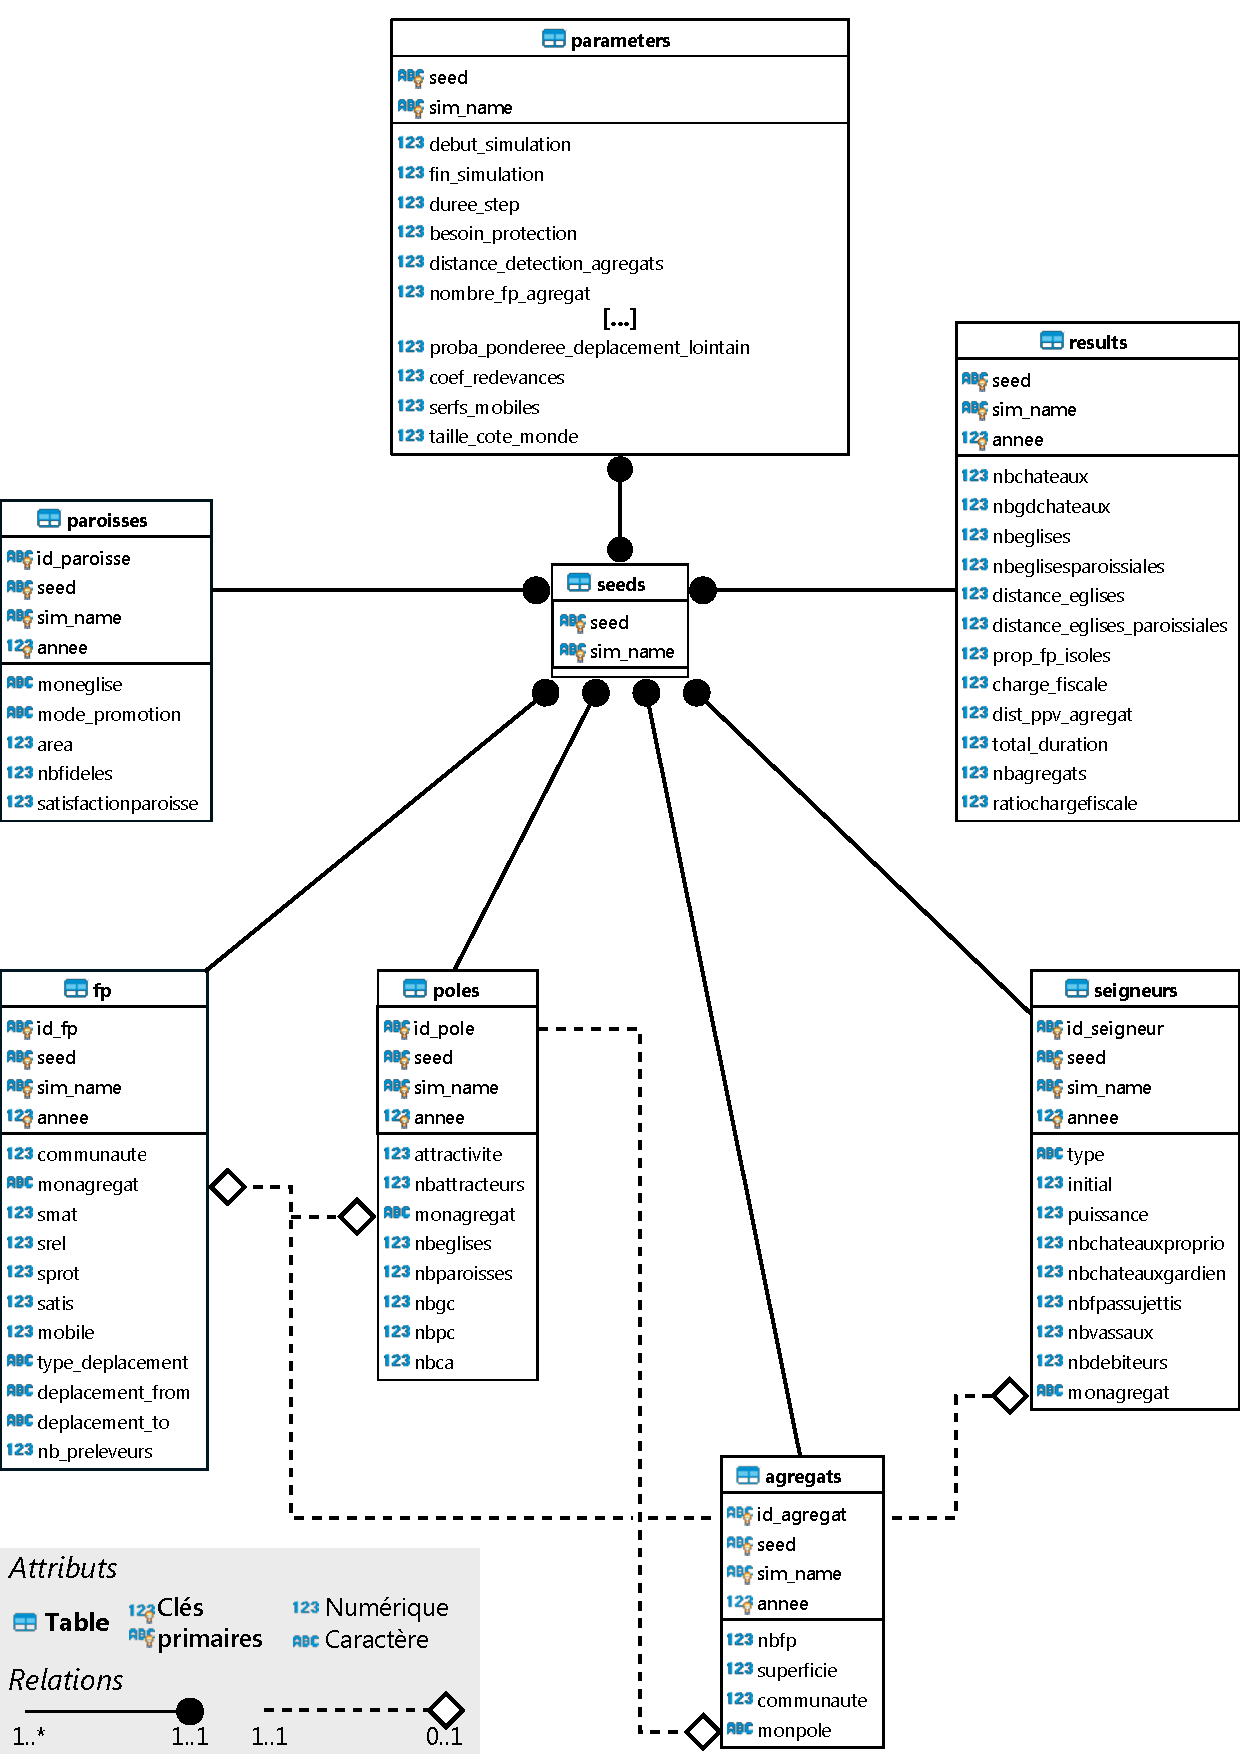
\includegraphics[width=\linewidth]{img/MCD_SimEDB_repris.pdf}
			\caption{Modèle Conceptuel de Données (MCD) des données en sortie de simulation de SimFeodal telles qu'implémentées dans SimEDB.}
			\label{fig:MCD_SimEDB}
		\end{figure}
\clearpage

\begin{figure}[H]
	\centering
	\captionsetup{width=\linewidth}
	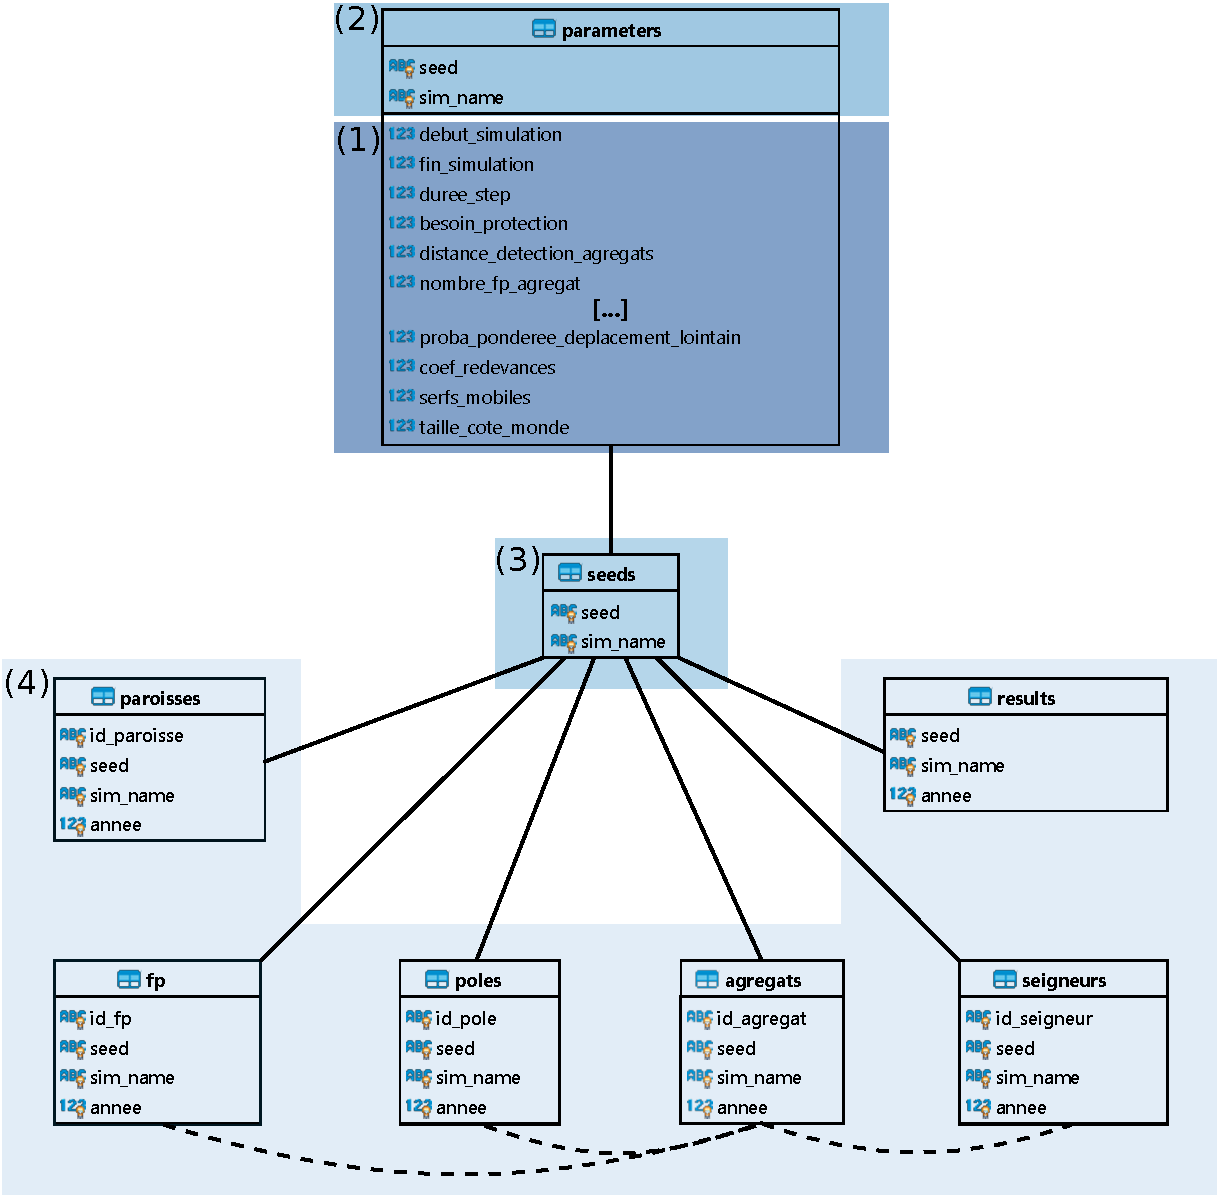
\includegraphics[width=\linewidth]{img/MCD_SimEDB_simplified.pdf}
	\caption{Les étapes d'interrogation de la BDD de SimEDB :\\
		(1) Filtrage d'un sous-ensemble de valeurs de paramètres ;
		(2) Les simulations associées sont isolées dans la table des paramètres;
		(3) Répercussion de ce filtre dans la table contenant les identifiants des simulations ;
		(4) Toutes les tables sont filtrées en répercussion}
	\label{fig:MCD_SimEDB_etapes}
\end{figure}
\clearpage
		\subsubsection{Un modèle de données pour favoriser l'interrogation et le filtrage conjoint}

		Le schéma choisit, et le Modèle Conceptuel de Données (MCD) associé, permettent donc une interrogation rapide des données en simplifiant les tâches d'agrégation et en minimisant la quantité de jointures nécessaires à la génération des indicateurs de sortie.

		Le choix de s'écarter légèrement du schéma en étoile présente un autre avantage, extrêmement utile, dans le cadre d'une exploration interactive des indicateurs de SimFeodal.
		En effet, comme on l'a vu auparavant (\cref{subsec:explorer-simedb}), dans SimEDB, on compare les simulations en les isolant à partir des valeurs de paramètres qui leur correspondent, via un acte de \textit{brushing} des valeurs de paramètres présentées dans un graphique en coordonnées parallèles interactif.

		Du côté du MCD, la table correspondante est la table \texttt{parameters}. Quand l'utilisateur sélectionne un sous-ensemble de valeurs de paramètres, la table est filtrée, et ne renvoi donc que les simulations correspondantes.

		C'est ici que l'intérêt de la table \texttt{seeds} et de son lien bidirectionnel avec la table \texttt{parameters} apparaît : une fois \texttt{parameters} filtrée, cette sélection est renvoyée à la table \texttt{seeds}, et se répercute donc directement à toutes les autres tables.
		Avec une unique requête, qui plus est sur une table de faible dimension (\texttt{seeds} ne comporte que deux champs), le filtrage est donc extrêmement véloce, accélérant d'autant le filtrage des autres tables et donc la génération des indicateurs de sortie.

		Ces étapes de filtrage successifs, optimisées par l'architecture choisie pour les données de SimFeodal, sont schématisées dans la \cref{fig:MCD_SimEDB_etapes}.


		\subsection*{Une organisation dédiée à l'exploration interactive}
		La présentation des choix d'organisation de données témoigne d'une visée résolument applicative, c'est-à-dire visant à penser l'organisation, la structuration et les SGBD d'implémentation, comme au service de la plate-forme d'exploration SimEDB.
		Le SGBD choisi, MapD, est ainsi un logiciel particulièrement adapté aux besoins identifiés, c'est-à-dire à une efficacité et une robustesse d'interrogation des données générées par SimFeodal.
		MapD est interrogeable de manière universelle, via des protocoles de connexion standards, au moyen d'un langage qui fait office de \textit{lingua franca} de l'interrogation de données, le SQL.
		Au sein du SGBD, la structure des données, révélée dans le MCD qui adopte une structure \og en étoile\fg{}, vise aussi à faciliter et à optimiser la vitesse des requêtes visant à générer les indicateurs de sortie de SimFeodal.
		Cette structure de données est enfin pensée, en amont, pour minimiser le nombre requêtes nécessaires à l'affichage des indicateurs, dans un cadre interactif, correspondant à des sous-ensembles des nombreuses simulations effectuées au cours de la construction, du paramétrage et de la calibration de SimFeodal.

		Il est important de noter qu'en l'absence de ces choix de conception de base de données, de la modélisation conceptuelle jusqu'à l'implémentation technique, la plate-forme d'exploration des données SimEDB, que nous allons maintenant présenter plus en détail, n'aurait pu être conçue, élaborée et bâtie de manière convaincante.

\clearpage
\section[Une plate-forme d'exploration de données de simulations : SimEDB]{Une plate-forme d'exploration de données de simulations : SimEDB%
 \sectionmark{SimEDB}}\label{sec:SimEDB}

La \cref{sec:explorer-sorties-simfeodal} (\cnameref{sec:explorer-sorties-simfeodal}) a décrit les étapes successives d'avancement dans l'exploration des données en sortie de SimFeodal, depuis l'observation en direct des simulations jusqu'au besoin d'une plate-forme permettant l'exploration et la comparaison interactive des sorties de simulation.
La plate-forme proposée en réponse à ce besoin, SimEDB\footnote{
	\textbf{Sim}Feodal \textbf{E}xploration \textbf{D}ash\textbf{B}oard, voir la note de bas de page \ref{ftn:origine-simedb}, \cpageref{par:introduction-nom-simedb}.
}, dans un objectif de généricité et d'adéquation, se devait aussi de répondre à de nombreuses contraintes, aussi bien liées aux possibilités offertes qu'à l'usage qui en serait fait.
Dans cette partie, nous nous attacherons donc à présenter les contraintes qui ont guidé la conception de SimEDB, ainsi que les choix, méthodologiques et techniques, qui en ont résulté.

	\subsection{Contraintes}

		\subsubsection{Adapter la complexité aux utilisateurs}

			Dans le domaine de l'Interface Homme-Machine (IHM), il est courant de considérer qu'un outil d'analyse et de représentation doit être adapté à un public. La \cref{fig:cartography3}, emblématique de la conception de géovisualisations par Alan MacEachren, replace ainsi les types d'usage d'une plate-forme d'exploration selon trois axes : les utilisateurs visés (\textit{users}), le niveau d'interaction souhaité (\textit{interaction}) et l'objectif poursuivi par la (géo)visualisation (\textit{task}).
			D'après ce schéma, à un niveau d'expertise de l'utilisateur correspond un unique degré d'interaction : plus l'utilisateur est expert du domaine, plus il s'attendra à disposer d'un outil complexe : \og All participants agreed that user expertise requires increased interface complexity, as suggested by the Cartography³ framework\fg{} \autocite[16]{roth_interactivity_2015}.

			\begin{figure}[H]
				\hspace*{\fill}%
				\begin{minipage}[t]{.46\linewidth}
					\centering
					\captionsetup{width=.9\linewidth}
					\vspace{0pt}
					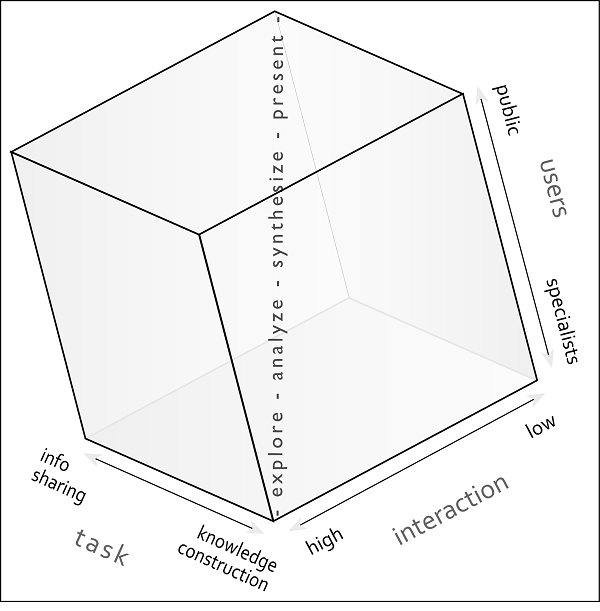
\includegraphics[width=\linewidth]{img/CV35-Fig2a-600.png}
					\caption{\og \textit{An update to Cartography³, 10 years after its conception}\fg{}, par \cite{coltekin_geovisualization_2018}, d'après \cite[10]{maceachren_geovisualization_2004}.}
					\label{fig:cartography3}
				\end{minipage} \hfill
				\begin{minipage}[t]{.46\linewidth}
					\centering
					\captionsetup{width=.9\linewidth}
					\vspace{0pt}
					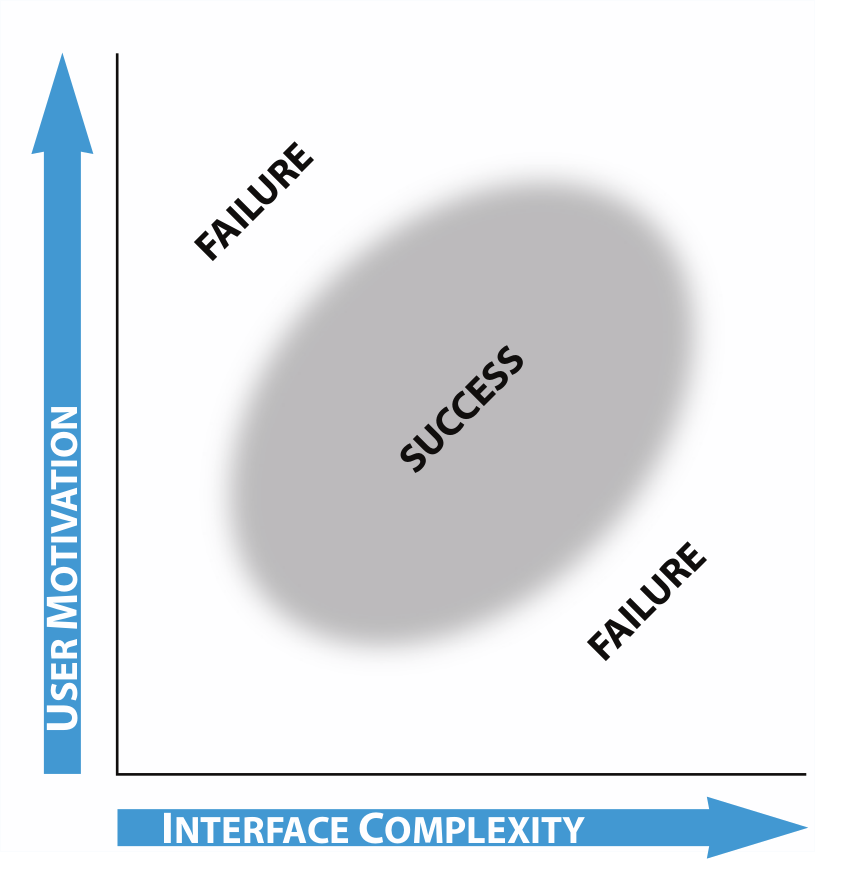
\includegraphics[width=\linewidth]{img/Roth_Interface_Complexity.png}
					\caption{\og \textit{Interface complexity versus user motivation. }\fg{}, \cite[79]{roth_interactive_2013}.}
					\label{fig:interface-complexity}
				\end{minipage}
			\end{figure}

			L'usage prévu de SimEDB -- nettement dans la construction de connaissance --, de même que le \og niveau\fg{} de ses utilisateurs -- expert dans le sens thématique et de la modélisation conceptuelle --, devraient donc logiquement, selon le schéma, bénéficier d'une forte complexité possible dans l'interaction.

			\paragraph*{Des utilisateurs hétérogènes mais captifs}

			SimEDB s'inscrit pourtant à un niveau intermédiaire, entre l'analyse et la synthèse : l'exploration, au sens entendu par MacEachren (\textit{explore}), est ici délaissée de par le choix de présenter des indicateurs spécifiés plutôt que de laisser l'utilisateur les assembler.

			Cet écart au modèle conceptuel de MacEachren s'explique notamment par la diversité des utilisateurs de SimEDB : qualifier un niveau d'expertise général serait absurde, tant les spécificités de cette expertise sont nombreuses : entre des profils de spécialiste thématiciens, de modélisateurs ou encore de géomaticiens, l'expertise est présente, mais concernant des champs différents, toutefois tous intéressés par l'exploration des sorties de SimFeodal.

			Il est dès lors peu évident de se fixer sur un degré de complexité à atteindre dans la plate-forme d'exploration : un niveau faible serait frustrant pour les utilisateurs avancés, et un niveau avancé serait source de confusion et donc de perte de motivation.

			Il nous était toutefois possible de miser sur une bonne motivation générale étant donné les circonstances particulières d'utilisation de SimEDB : contrairement à une utilisation grand public, qui ne présente aucun engagement vis-à-vis d'une interface d'exploration de données, ou à l'inverse contrairement à des domaines experts où chaque utilisateur dispose de ses propres outils et méthodes pour explorer un jeu de données, le public cible de SimEDB est \og captif\fg{}, c'est-à-dire qu'il ne dispose pas d'autre solution que de passer par cette plate-forme pour explorer les données, en particulier en raison des contraintes liées à ces données (cf. \cref{subsec:donnees-indicateurs}, \cnameref{subsec:donnees-indicateurs} par exemple).

			Dès lors, la motivation des utilisateurs ne peut qu'être importante, et l'interface a la possibilité de devenir plus complexe tout en se révélant adaptée (\cref{fig:interface-complexity}).

			\paragraph*{Intuititivé de l'usage au regard des applications traditionnelles}

			En dépit de cette motivation, les utilisateurs de SimEDB demeurent majoritairement des experts thématiciens, potentiellement peu familiarisés à l'exploration de données interactives.
			Afin que le temps d'exploration des données issues de SimFeodal soit dévoué à la compréhension et à la synthèse de ces données plutôt qu'à un apprentissage ou amélioration en exploration de données, il a été choisi de créer une application aussi simple que possible au regard des fonctionnalités principales qu'elle devait permettre : observer les indicateurs de sortie de simulation pour des expériences données, et les comparer entre elles aussi efficacement que possible.
			Il n'était donc pas question de construire un nouveau \og logiciel expert \fg{}, doté de dizaines de fonctionnalités avancées, mais au contraire, de simplifier au maximum l'interface pour ne pas encombrer et complexifier l'utilisation de ces fonctionnalités principales.
			On souhaitait une plate-forme aussi épurée que possible, plutôt que de partir, par exemple, sur la personnalisation et adaptation de l'un des outils d'exploration existants et dédiés à offrir une forte possibilité de manipulation.

		\subsubsection{Efficacité}

		Dans la description du choix du SGBD, on a mentionné une première fois l'intérêt de disposer d'une solution d'interrogation de données permettant une rapidité de l'exécution des requêtes.
		Sans entrer dans le détail des recherches en IHM, on peut toutefois caractériser cet intérêt par deux aspects complémentaires, une solution interactive minimisant les latences permettant (1) de conserver l'utilisateur, c'est-à-dire de ne pas le décourager d'utiliser l'application, et (2) de lui faire conserver sa concentration (\textit{focus}), c'est-à-dire que le délai entre son interaction et la réponse graphique soit suffisamment court pour que l'identification effectuée par son système cognitif ne soit pas affecté.
		
		Le premier point a été abordé plus haut (\cref{subsubsec:interroger-robuste-efficace}), et surtout, en raison de la \og captivité\fg{} de l'utilisateur évoquée ci-dessus, ne s'applique que marginalement à notre cas d'étude : si des délais trop importants pourraient décourager l'utilisateur, l'absence d'alternative utilisable pour explorer ces données les contraint toutefois à faire usage de la plate-forme d'exploration pour comprendre le comportement du modèle SimFeodal.

		\paragraph*{Conserver la concentration}
		
		Le problème de la concentration de l'utilisateur demeure, lui, critique : des études ont montré, depuis longtemps \autocite{mackenzie_lag_1993}, qu'il y avait un lien fort entre la performance d'une interrogation visuelle et le délai nécessaire à son obtention.
		\cite[8]{liu_effects_2014} montrent ainsi qu'avec un simple délai de $500ms$, la qualité des observations, des généralisations qui peuvent être tirées des données, et des des hypothèses émises, décroît nettement. Les auteurs indiquent d'ailleurs que ces effets sont plus importants encore quand l'exploration est effectuée par des actions de \textit{brushing} et de sélections croisées (\textit{linking}), deux méthodes qui sont au cœur de SimEDB : \og For example, more aggressive caching or prefetching methods may be employed for operations sensitive to small variations in latency, such as brushing and linking \fg{}\autocite[9]{liu_effects_2014}.
		
		\cite{forch_are_2017}, pour leur part, étudient la perception du délai de réponse lors d'interactions menées avec une souris d'ordinateur. Ils concluent ainsi que les utilisateurs perçoivent des délais d'attente inférieurs à $100ms$, mais notent que les utilisateurs n'en sont pas pour autant perturbés, en particulier ceux qui ont le moins l'habitude de réactions rapides\footnote{
		Ils remarquent ainsi que les utilisateurs plus habitués à des jeux vidéos rapides (\og highly dynamic computer games, such as action games, racing games, or first person shooter games [...]\fg{}, \cite[51]{forch_are_2017}) sont plus vite affectés par le délai de réponse que les autres.
		}.
		
		Concernant le champ, plus spécifique, des \textit{visual analytics}, nous n'avons pas trouvé d'articles de référence permettant d'établir une comparaison de l'efficacité des résultats trouvés selon la latence de la réponse.
		Les auteurs de ce champ recommandent de prêter attention à la rapidité de rendu et à son optimisation, mais sans que ne trouvions de résultats plus précis :
		\begin{quotation}
			\og
			When simple pattern finding is needed, the importance of having a fast, highly interactive interface cannot be emphasized	enough. If a navigation technique is slow, then the cognitive costs can be much greater than just the amount of time lost, because an entire train of thought can become disrupted by the loss of the contents of both visual and nonvisual working memories.
			\fg{}\\
			\mbox{}~ \hfill  \cite{ware_information_2012}, tiré de \cite[12]{amirpour_amraii_human-data_2018}.
		\end{quotation}

		Tout au plus pouvons-nous émettre l'idée qu'il serait évident que la latence acceptée dans un environnement graphique de ce type soit largement supérieure à celle des environnements virtuels (réalité augmentée, visualisations immersives\ldots), sans pour autant que nous ne puissions quantifier cet écart.
		\cite[74]{shneiderman_designing_2004} indiquent tout de même, parmi les \og 8 règles d'or du design d'interfaces\fg{} un délai maximal pour une phase d'exploration, sur lequel nous pouvons construire une estimation : \og \textit{Reduce short-term memory load.} The limitation of human information processing in short-term memory (\textbf{the rule of thumb is that humans can remember ``seven plus or minus two chunks'' of information}) requires that displays be kept simple, multiple-page displays be consolidated, window-motion frequency be reduced, and sufficient training time be allotted for codes, mnemonics, and sequences of actions.\fg{}.
		Si l'on considère qu'une session d'exploration requiert l'étude d'une dizaine d'indicateurs, et que chacun demande une quinzaine de secondes d'analyse visuelle, alors le temps d'attente entre les visualisations ne doit pas dépasser deux à trois secondes.
	
		Selon ces différentes considérations, dans le cadre de SimEDB, on doit donc viser à développer une plate-forme aussi rapide que possible, tout en sachant, dès le départ, qu'il sera impossible d'arriver aux délais de $100ms$ ou $500ms$ évoqués précédemment, ne serait-ce que parce que le temps de requête des données -- sans compter le temps de rendu graphique -- est déjà supérieur d'un ordre de grandeur.

		\subsubsection{Interopérabilité et évolutivité}
		
		Une autre contrainte forte tient cette fois au choix de l'environnement informatique qui accueillera la plate-forme d'exploration.
		On peut résumer ce choix à deux alternatives : un environnement local, en installant l'application sur l'ordinateur de chaque utilisateur, ou un environnement distant, où l'application serait donc accessible à distance, par exemple via une interface web.
		
		Ce choix a des nombreuses répercussions, aussi bien en matière de possibilité d'accès que de facilité à faire évoluer la plate-forme.
		Le choix le plus classique est de développer une application installable sur un ordinateur : cela permet de garantir une utilisation à tout moment, sans contrainte d'accès au réseau internet, et cela permet aussi d'obtenir de meilleurs performances, puisque la rapidité de l'application dépendrait uniquement de la puissance de l'ordinateur plutôt que de devoir souffrir du passage par l'intermédiaire d'un serveur.
		
		\paragraph*{Différents supports d'interrogation}
		La performance d'une application locale, par rapport à une application distante, est un atout extrêmement intéressant, comme on vient de le montrer plus haut.
		Pourtant, cela implique une énorme contrainte : l'application doit être interopérable entre les différents systèmes d'exploitations (\textit{Operating System}, OS) et versions de ceux-ci.
		Les utilisateurs potentiels de SimEDB, représentation fidèle des acteurs de la recherche, se partagent ainsi entre les trois systèmes d'exploitations majoritaires (Windows, MacOs, Linux).
		
		Pour permettre à chacun d'utiliser SimEDB, il faudrait donc que le développement de cette plate-forme soit compatible avec ces différents OS, ce qui est une contrainte considérable en développement logiciel.
		
		Ne mentionnons même pas les nouveaux OS, centrés autour d'usages tactiles, tels qu'on les retrouve sur les tablettes et autres \textit{smartphones}, qui demandent, eux aussi, de nombreuses spécificités de développement.
		
		En somme, disposer d'une application locale universelle, c'est-à-dire utilisable quelque soit le support informatique, est une quasi-impossibilité technique, et un objectif en soit, que notre travail de recherche ne cherche aucunement à résoudre.
		Pour garantir la faisabilité d'une plate-forme d'exploration de données locale dédiée aux données de simulation de SimFeodal, il faudrait donc commencer par restreindre son champ d'application à un ou deux supports officiels, par exemple l'OS Windows, abandonnant de fait les utilisateurs potentiels ne disposant pas de cette architecture logicielle.
	
		\paragraph*{Gérer les mises à jours et modifications}
		
		Comme pour les bases de données (\cnameref{par:stockage-centralise}, \cpageref{par:stockage-centralise}), la question de l'application locale ou distante pose un contrainte supplémentaire en matière de maintenabilité et d'évolutivité de la plate-forme choisie : dans le cadre d'une application locale (correspondant au distribué en SGBD), la distribution des différentes mises à jour de l'application entraînent nécessairement l'installation locale, à chaque fois.
		Le risque est alors que tous les utilisateurs ne disposent pas d'une même version, ce qui peut entraîner, par exemple, des contradictions dans l'évaluation d'expériences, certains utilisateurs ayant accès à une version \og buggée\fg{}.
		
		Sans aller jusqu'à ces extrêmes, notons qu'avec une application locale, le temps de répercussion d'une modification du code de la plate-forme est plus important : il faut en effet réinstaller sur chaque poste le logiciel ainsi modifié.
		Cela disqualifie de fait des modifications \og en direct\fg{}, par exemple lors d'une session collective d'exploration des résultats où les utilisateurs auraient des propositions de modifications à faire, ne serait-ce que pour des changements aussi infimes que des titres de graphiques ou d'axes.
		
		\paragraph*{Le choix d'une application web}
		
		Au contraire, avec une application distante, donc basée sur l'accès, par un navigateur internet, à une application centralisée, ces problèmes ne se posent pas : des navigateurs sont disponibles pour tous les OS existants (OS dédiés aux ordinateurs ou aux usages mobiles), et interprètent de la même manière une page web, indépendamment de leur support de consultation.
		De plus, comme pour les SGBD, l'usage d'une plate-forme distante permet une répercussion instantanée des mises à jour et corrections : un utilisateur n'a qu'à rafraichir sa page pour que la dernière version de l'application s'affiche.
		De la même manière, si un utilisateur souhaite étudier un nouvel indicateur, non prévu auparavant, le temps de déploiement peut être suffisamment court pour que cela soit possible au cours d'une même session d'exploration de données.
		
		Il y a toutefois un désavantage certain, puisque les données permettant l'affichage des indicateurs doivent transiter sur le réseau internet : l'application n'est donc pas disponible hors-connexion, et, en cas de connexion lente, sera particulièrement éprouvée.
		Cette lenteur relative est toutefois compensée par un avantage à la centralisation de l'application : les calculs, parfois lourds, ne reposent pas sur les capacités individuelles des ordinateurs clients.
		En installant l'application sur un serveur dédié, il suffit donc d'augmenter les caractéristiques de celui-ci pour que les performances soient améliorées pour chacun des utilisateurs de l'application.
		
		Dans le cas de SimEDB, nous disposons de ressources informatiques largement suffisantes (serveur de calcul interne à l'UMR Géographie-cités dans un premier temps, puis serveur de calcul partagé via la \og Très Grande Infrastructure de Recherche\fg{} -- TGIR -- Huma-Num) pour assurer une rapidité de traitement des données et ainsi permettre à l'application SimEDB de se dégager de ce \og goulot d'étranglement\fg{} technique qu'aurait sinon éprouvée la plate-forme.
			
		\subsubsection{Généricité de l'interrogation et indépendance aux données}
		
		La dernière contrainte, plus technique, tient au besoin de généricité d'une plate-forme d'exploration de données vis-à-vis des données qu'elle interroge.
		On a résumé les possibilités et choix effectués en matière de SGBD (\cref{subsec:capacite-interrogation} :  \cnameref{subsec:capacite-interrogation}), et décidé de ne retenir que des SGBD permettant une interrogation standardisée via des connecteurs génériques et un langage universel (le SQL).
		
		L'infrastructure de stockage et d'organisation des données a ainsi été conçue pour être aussi générique que possible.
		Encore faut-il que la plate-forme d'exploration de données soit elle aussi aussi générique que possible, et donc en mesure de profiter de l'universalité du SGBD choisi.
		
			\paragraph*{Indépendance au support de données}
		Une contrainte forte est donc constituée par la capacité de la plate-forme a être indépendante de la source des données : quelque soit le SGBD choisi, les requêtes émises par la plate-forme doivent être les mêmes, sans requérir d'adaptations spécifiques en dehors de la désignation du lieu de stockage des données	et des pilotes du SGBD.
		
		Dans les faits, lors de la construction de SimEDB (cf. \cref{sec:explorer-sorties-simfeodal} : \cnameref{sec:explorer-sorties-simfeodal}), plusieurs solutions de stockage de données ont été utilisés successivement : de simples fichiers csv au départ jusqu'au SGBD ultra-performant MapD, en passant par des solutions plus classiques intermédiaires (SQLite et MonetDB notamment).
		
		Il n'était donc aucunement question d'avoir à modifier le code source permettant de générer les indicateurs depuis les données, mais au contraire, de s'assurer d'utiliser des bibliothèques logicielles indépendantes des données, c'est-à-dire capables d'exécuter les mêmes chaînes de traitements quelque-soit la provenance des données.
		
			\paragraph*{Indépendance aux requêtes et modularité de l'implémentation}\label{par:DSL}
			
			Pour garantir cette généricité, il est donc nécessaire de s'assurer que le mode de communication de la plate-forme vers les données soit bien basé sur un langage universel : le SQL.
			Il convient donc de choisir un ensemble de technologies permettant de générer des requêtes SQL, quand bien même l'expression de ces requêtes elles-mêmes serait conçue dans un autre langage.
			Faire appel à un langage intermédiaire, générant du SQL en sortie depuis une entrée sous forme d'un \og \textit{Domain Specific Language}\fg{} (DSL) permet ainsi de bénéficier d'une part de l'universalité du SQL, et d'autre part, d'une syntaxe plus expressive que celle du SQL.
			Pour les requêtes complexes, le SQL tend ainsi a être peu lisible, les opérations s'emboîtant les unes dans les autres de manière très linéaires, et donc, souvent verbeuses.
			En SQL pur, il est donc peu évident de créer une implémentation modulaire d'une requête, c'est-à-dire permettant une factorisation des commandes et un paramétrage des entrées.
			
			Les indicateurs de sortie de SimFeodal sont pourtant, on l'a vu, assez fréquemment basés sur le même type d'opération : variation du nombre moyen d'agents au cours du temps de la simulation, courbes rang-taille des hiérarchies d'un type d'agent etc.
			Dans le cas du premier exemple, en SQL, pour passer d'une requête permettant de récupérer le nombre de foyers paysans au cours du temps, groupés par année et avec un filtre sur certaines simulations, il ne faut que quelques lignes de code. Pour adapter cette requête à l'interrogation du nombre d'agrégats, dans les mêmes conditions d'agrégation et de filtrage, l'effort est minime, mais peu évident à paramétrer pour rendre cette démarche plus générique.
			
			En utilisant un DSL, plus adapté à la manipulation de données qu'à la sélection de sous-ensembles, on gagne donc en modularité d'implémentation , et donc en ré-utilisation de fonctions plus génériques, ce qui permet de disposer d'un code-source plus robuste, ré-utilisable et évolutif.
			
			\subsubsection*{Conclusion : Vers une plate-forme web générique et intuitive}
			
			Il ressort de ces différentes contraintes et choix d'utilisation que les choix techniques, propres aux modalités d'interrogation des bases de données, mais aussi méthodologiques, au regard de la conception d'une interface graphique intuitive, imposent des restrictions assez conséquentes sur les possibilités techniques disponibles pour la conception de la plate-forme SimEDB.
			En premier lieu, on fait le choix de se tourner vers une plate-forme implémentée sous forme d'application web, utilisable depuis un simple navigateur -- donc inter-opérable entre les différents supports technologiques --, ce qui exclue de fait quantités d'outils, de logiciels et de bibliothèques logicielles pensées pour l'exploration interactive de données.
			On souhaite de plus que la plate-forme utilisée dispose d'une interface aussi épurée que possible, donc nécessairement très adaptée au cas particulier des données issues de SimFeodal, ce qui là aussi élimine un ensemble de solutions \og clefs-en-main\fg{}, par exemple conçues autour des \og webSIG\fg{} ou de bibliothèques logicielles de visualisations interactives intégrées.
			L'utilisation de la plate-forme doit être aussi efficace que possible, en cherchant à minimiser les temps de latence entre sélection interactive et affichage des indicateurs en résultant.
			On devra donc privilégier des ensembles technologiques récents et performants, intrinsèquement dédiés à l'interactivité, au détriment de \textit{frameworks} plus génériques, conçus pour une forte diversité d'usage plutôt que pour la tâche très spécifique que constitue la manipulation interactive de données.
			Enfin, il faut que cette solution, dans la mesure du possible, soit en mesure de proposer une syntaxes d'interrogation de données modulaire, factorisée, et plus expressive que le SQL qu'elle doit pourtant réussir à générer.
			

	\subsection{Construire une plate-forme interactive pour l'évaluation de SimFeodal}
	
	Dans cette dernière sous-partie, nous allons donc présenter les choix -- techniques, esthétiques et interactifs -- qui ont été adoptés dans la conception et l'implémentation de SimEDB.
	Nous les présentons ici de manière linéaire, dans l'ordre quasi-chronologique du développement, mais il est important de garder en considération que ces éléments sont intimement intriqués : un choix technique conditionne les types d'interactions possibles, l'utilisation de telle méthode d'interaction peut restreindre l'étendue des possibles techniques etc.
	
	Notons enfin que l'application SimEDB présentée ici, aussi bien dans son usage que dans sa conception, représente un instantané de développement, qui correspond à la période de rédaction du présent chapitre :
	à l'instar d'un modèle, une plate-forme peut et doit évoluer pour s'adapter aux besoins de ses utilisateurs tant qu'elle est utilisée.
	Les technologies et choix esthétiques introduits n'ont pas toujours été présents, et auront sans doute à évoluer dans la suite de la \og durée de vie\fg{} de SimEDB.
	
		\subsubsection{Choix des technologies}
		
	Nous présentons ici les technologies mobilisées dans le cadre du développement de SimEDB.
	Le but n'est pas d'entrer dans les détails de l'implémentation\footnote{
	Le code source de SimEDB -- et l'historique de son versionnement -- sont, pour cela, disponible en ligne sous licence libre, sur la plate-forme Github : 
	\faGithub~\href{https://github.com/RCura/SimEDB}{github.com/RCura/SimEDB}
	}, mais bien de justifier et présenter les choix relatifs aux technologies employées, en restant donc à un niveau assez général\footnote{
		À ce titre, les quelques lignes de codes présentes par la suite servent un but illustratif et descriptif, et nous semblent remplir ce rôle bien plus efficacement que n'importe quel schéma structurel ne le pourrait.
	}.
	Il nous paraît important d'entrer dans ces choix qui relèvent plus de la technique que de la méthodologie en ce qu'ils concourent de la volonté de reproductibilité de la thèse, et particulièrement de la reproductibilité de la démarche, conceptuelle et méthodologique, mise en place.
	Nous portons la conviction que l'ensemble de technologies assemblées ici dans notre \og chaîne de traitement\fg{} est très largement ré-utilisable, dans le cadre d'adaptations à d'autres cas d'études, mais aussi et surtout, pour une multitude de problématiques requérant une évaluation visuelle de données massives (\hl{on y reviendra dans le chap 7}).

	\paragraph*{Technologies webs \og natives\fg{}  et adaptativité}
	
	Au cours de la dernière décennie, les interfaces physiques de consultation de médias informatiques se sont largement diversifiées.
	Cela a provoqué une hétérogénéisation importante aussi bien des modes d'interaction (dispositifs \og tactiles\fg{}) que des modes d'affichages (les tailles et résolutions des écrans n'ont jamais été aussi diverses et imprévisibles).
	En conséquence, les normes de présentations graphiques ont évolué, vers plus d'\fg{}adaptativité\fg{}, en particulier avec l'avènement du \og responsive web design\fg{} (\og conception de sites web adaptatifs\fg{}) qui permet de prévoir efficacement l'agencement d'une page web quelque soit le support de consultation.
	
	Ces technologies, aujourd'hui indispensables, reposent sur des codes standardisés, verbeux et peu explicites, qui peuvent être générés à la volée par des \textit{frameworks} graphiques qui en simplifient l'usage.
	
	Les technologies plus lourdes qui prédominaient dans la réalisation d'applications web interactives il y a quelques années (\texttt{Adobe Flash}, \textit{applets} Java\ldots) sont donc maintenant assez peu universelles et le niveau de développement de standards tels que le langage et environnement HTML5 a suffisamment augmenté pour pouvoir justifier de s'en passer.
	
	Nous avons donc fait le choix de nous concentrer sur des environnements standardisés, capables de générer du \texttt{HTML} (\og \textit{HyperText Markup Language}\fg{}), lui-même mise en forme à l'aide de styles \texttt{CSS} (\og \textit{Cascading Style Sheets}\fg{}) et rendu interactif par du code \texttt{JavaScript}.
	
	À ce titre, le framework \texttt{Bootstrap}\footnote{\href{http://getbootstrap.com/}{http://getbootstrap.com/}} s'est révélé extrêmement utile dans le \textit{design} de l'interface de SimEDB (et des versions précédentes), tant il simplifie l'expressivité d'une mise en page à l'aide d'une grille graphique et de composants interactifs ré-utilisables.
	
	\paragraph*{Le choix d'environnements de développement intermédiaires}
	
	\hl{Ne pas oublier, dans le positionnement (chap1) de consacrer au moins un paragraphe (ou encadré) au choix \og militant\fg{} de ne se tourner QUE vers des outils libres, sans exception.}
	
	Pour construire des applications interactives en lignes, de multiples choix sont possibles, et l'on peut les catégoriser selon le niveau de développement qu'ils demandent.
	
	Par exemple, il est tout à fait possible de s'appuyer sur des briques logicielles de bas niveau (ce que l'on appelle communément \textit{framework}), et de développer à partir de celles-ci toute l'interface et le fonctionnement d'une application, par exemple au sein de \textit{frameworks} \og MVC\fg{} (Modèle-Vue-Contrôleur).
	Cette approche, majoritaire dans la construction d'applications actuelles (avec des \textit{frameworks} JavaScript tels que \texttt{ReactJS} ou \texttt{AngularJS}, ou encore Python tels \texttt{Django} ou \texttt{Flask}), est extrêmement flexible et performante, au prix d'un développement important : le \textit{framework} fournit des \og briques\fg{} logicielles de base -- les composants --, très génériques, qui doivent être largement adaptées.
	La communication entre ces composants doit être entièrement prévue et implémentée, et on abouti donc nécessairement sur des projets assez importants, qui demandent une réelle expertise en développement et portent le risque d'être trop complexes pour être facilement adaptés et donc génériques.
	
	À l'autre bout du gradient de développement, on peut aussi choisir de bâtir une application à partir d'un ensemble logiciel intégré, comme \texttt{Tableau}, qui permet d'agencer visuellement et graphiquement des composants graphiques et leurs liens. Ces outils, très usités en informatique décisionnelle, sont extrêmement simples à prendre en main, y compris pour des \og utilisateurs finaux\fg{} -- analystes par exemple --, mais sont en contre-partie bien moins personnalisables, adaptables, et sont majoritairement des logiciels propriétaires, donc non adaptables.
	
	Entre ces deux extrêmes, quelques \textit{frameworks} intermédiaires, souvent originaires des outils de manipulation de données plus que du monde de l'informatique décisionnelle, mettent à disposition de l'utilisateur des composants de plus haut-niveau que les \og briques élémentaires\fg{}, où l'interaction entre les composants est déjà pré-conçue, tout en reposant sur une construction \og depuis zéro\fg{}, donc personnalisables et adaptables.
	Généralement, chaque \textit{framework} est associé à un langage de programmation : \texttt{Shiny}\footnote{\href{https://shiny.rstudio.com/}{https://shiny.rstudio.com/} -- \cite{chang_shiny_2015}} pour le langage \texttt{R}, \texttt{Dash}\footnote{\href{https://plot.ly/products/dash/}{https://plot.ly/products/dash/} -- \cite{plotly_introducing_2017}} pour le langage \texttt{Python} et \texttt{Escher}\footnote{\href{http://escher-jl.org/}{http://escher-jl.org/}-- \cite{gowda_escher_2018}, d'après \cite{bezanson_julia_2014}} pour le langage \texttt{Julia}.
	
	Le choix de tel ou tel framework dépend certes de la maturité de chaque projet -- Shiny est à ce titre très en avance --, mais surtout du langage informatique que le concepteur de l'application souhaite utiliser.
	Dans le cas de SimEDB, le créateur de la plate-forme est adepte du langage R (voir \cite{commenges_r_2014}) et pratique l'environnement Shiny depuis plusieurs années (voir \cite{cura_creer_2015}) : le choix d'utiliser ce framework était donc assez évident.	
	
	\paragraph*{Manipuler les données avec \texttt{R} et \texttt{dplyr}}
	
	Les langages de programmation, et en particulier les plus utilisés en analyse de données, reposent souvent sur une architecture logicielle modulaire : le langage constitue un cœur, autour duquel des bibliothèques logicielles (des \textit{packages} en R) viennent ajouter des fonctionnalités.
	Parmi ces bibliothèques logicielles, en Python comme en R, certaines sont entièrement dédiées à la manipulation de données tabulaires, on parle alors de \og Data Manipulation Language\fg{} (DML) et permettent d'effectuer des traitements avec des approches fonctionnelles, plutôt qu'avec les structures impératives plus fréquemment utilisées en programmation.
	En R, ces \textit{packages} constituent de véritables écosystèmes, dotés de leur propre DSL (voir \cnameref{par:DSL}, \cpageref{par:DSL}) et donc d'une grammaire de manipulation de données propre.
	
	L'un de ces \textit{packages}, \texttt{dplyr} \autocite{wickham_dplyr_2015}, s'inscrit dans un écosystème dénommé \texttt{tidyverse} \autocite{wickham_tidyverse_2017}, et permet ainsi de chaîner des opérations de manipulation de données en une chaîne de traitement complète, plutôt que de faire appel aux habituelles boucles de parcours de matrices propres aux langages de programmation classiques.
	Ce faisant, avec des opérations chaînées, qui reposent sur des \og verbes\fg{} permettant d'effectuer des traitements de restructurations, de modification, de filtrage ou d'enrichissement d'une donnée tabulaire, on obtient un ensemble d'instructions qui forment une \og phrase\fg{} de manipulation de données, exprimées donc dans la \og grammaire de traitement de données\fg{} fournie par \texttt{dplyr}.
	Cette \og grammaire\fg{} s'inspire notamment du SQL, bien que beaucoup plus complète, et peut en particulier être \og convertie\fg{} en SQL (\cref{fig:dml-simedb}), c'est-à-dire qu'une suite d'instructions exprimées via dplyr en R (\cref{subfig:exemple-dplyr-R}) peut être traduite en SQL (\cref{subfig:exemple-dplyr-SQL}), et donc envoyée et exécutée sur un SGBD.
	
	En matière de performance, l'approche de \texttt{dplyr} est intéressante : toutes les opérations sont effectuées par le SGBD directement, et seul le résultat final est renvoyé à R (instruction \texttt{collect()}).
	Le traitement de données bénéficie donc de la rapidité d'exécution du SGBD MapD, tout en profitant de la syntaxe expressive de \texttt{dplyr}.

		\begin{figure}[H]
			\centering
			\hspace{5pt}
			\subfloat[Code source R avec le \textit{package} \texttt{dplyr}]{\label{subfig:exemple-dplyr-R}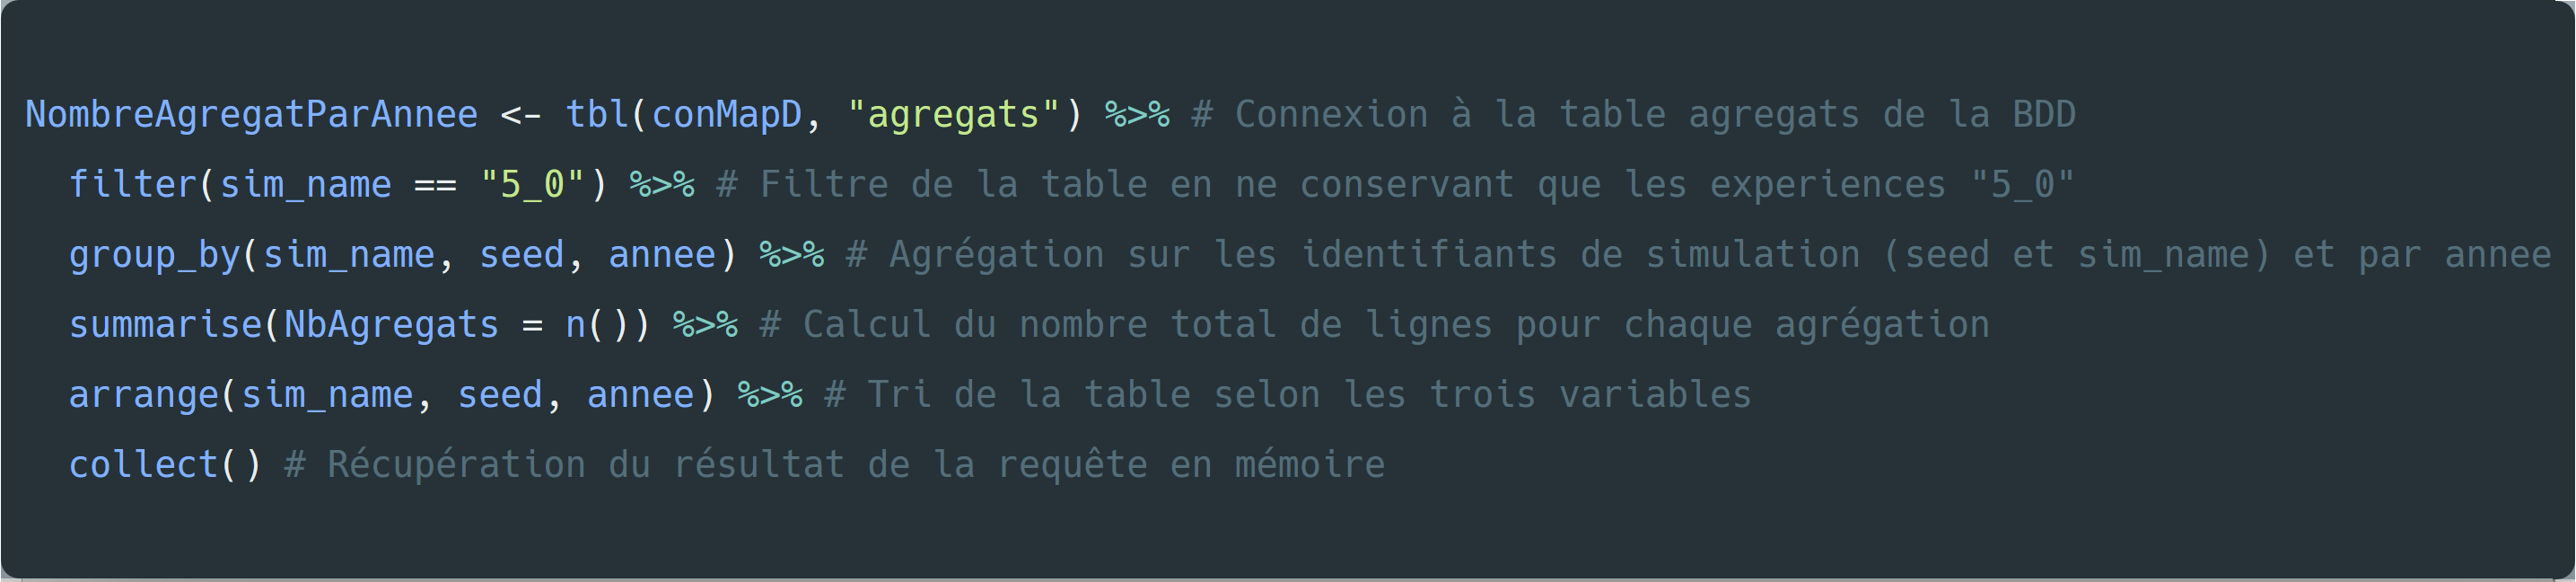
\includegraphics[width=\linewidth]{img/dplyr_cut.png}}
			\hspace{5pt}
			\subfloat[Traduction du code source \texttt{dplyr} en \texttt{SQL}]{\label{subfig:exemple-dplyr-SQL}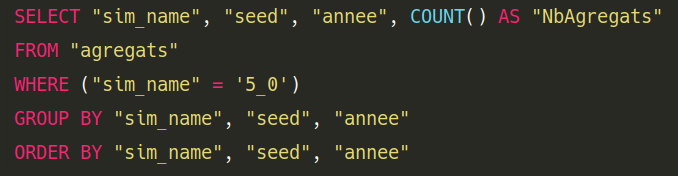
\includegraphics[scale=.35]{img/SQL_Sublime.png}}
			\caption{Un exemple de manipulation de données stockées dans un SGBD depuis R. On y interroge la table des agrégats de population pour calculer le nombre moyen d'agrégats par année de simulation.}
			\label{fig:dml-simedb}
		\end{figure}

	\clearpage
	\paragraph*{Création de graphiques avec \texttt{ggplot2} et la \og \textit{grammar of graphics}\fg{}}
	
	\paragraph*{}
	\begin{wrapfigure}{l}{.42\linewidth}
		\centering
		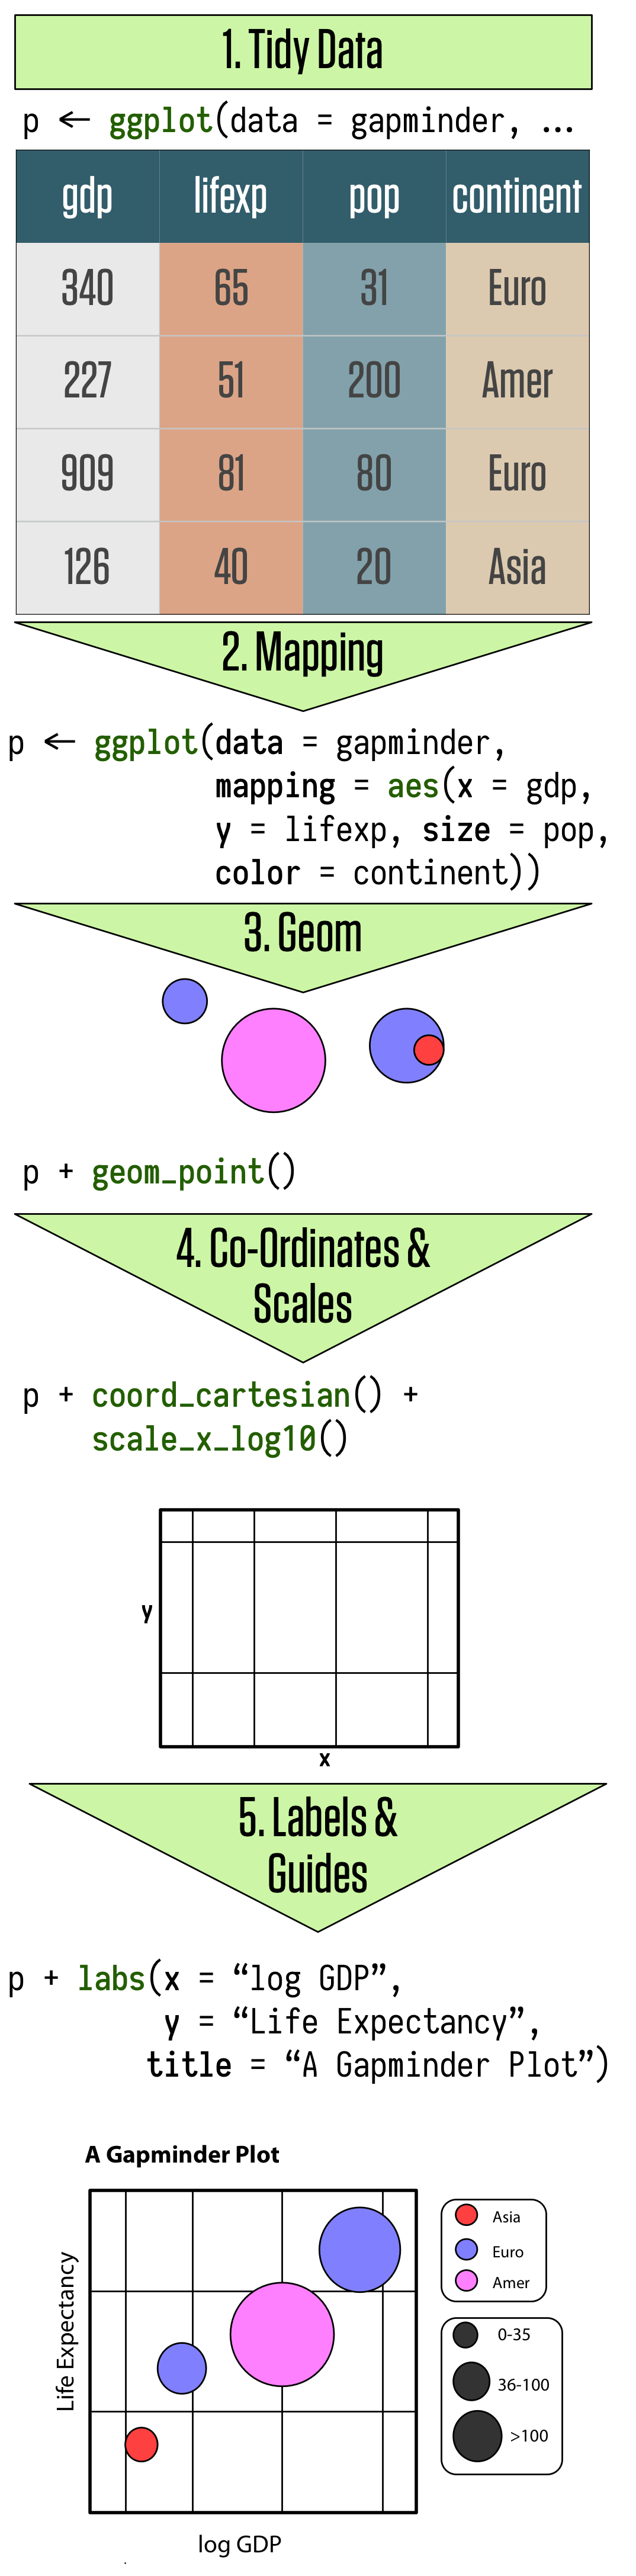
\includegraphics[width=.92\linewidth]{img/ch-03-ggplot-flow-vertical.png}
		\caption{Représentation des éléments de grammaire de \texttt{ggplot2}, tiré de \cite{healy_data_2018}.\\
			\hl{Ré-organiser proprement le graphique}%
		}
		\label{fig:socviz-ggplot2}
	\end{wrapfigure}
	Une fois les données pré-traitées, encore est-il nécessaire de construire les indicateurs graphiques de sortie de simulation.
	Pour cela, il existe de nombreux \textit{packages} pour R dédiés à la représentation graphique.

	L'un des \textit{packages} les plus utilisés, \texttt{ggplot2} \autocite{wickham_ggplot2_2016}, met en œuvre une syntaxe assez adaptée à nos contraintes : ce \textit{package} est conceptuellement fondé sur la \og \textit{grammar of graphics}\fg{}, c'est-à-dire une vision modulaire et très structurée de la conception graphique, pensée par Leland Wilkison \autocite{wilkinson_grammar_2006}.
	La logique, assez familière pour un utilisateur de Systèmes d'Information Géographique (SIG), consiste à penser une représentation graphique comme un ensemble de couches (\textit{layers}), qui se superposent, se complètent, et sont toutes basées sur une source de données.
	Les différentes composantes des données (variables par exemple) sont associées à des composantes graphiques de base (abscisse, ordonnée, taille, couleur \ldots), formant ainsi une \og cartographie\fg{} (\textit{mapping}) des données avec les composants graphiques (voir \cref{fig:socviz-ggplot2}).

	Pour SimEDB, l'un des intérêts principaux de créer les indicateurs graphiques est justement cette grammaire, extrêmement structurée, qui permet donc de ré-utiliser largement les codes-sources écrits pour un indicateur et de les adapter aisément à d'autres indicateurs.
	Par exemple, de nombreux indicateurs de sortie de SimFeodal montrent l'évolution du nombre d'agents au cours des années de simulation (\cref{fig:exemple-ggplot2-simedb}).
	Ce type de graphique est rapide à produire avec \texttt{ggplot2} -- il ne requiert que quelques lignes de code (\cref{subfig:exemple-ggplot2-R}) --,
	et en changeant le tableau de données en entrée (créé dans \cref{subfig:exemple-dplyr-R}), reproduit exactement le même type de graphique pour, par exemple, un autre type d'agent.
	Le \textit{package} \texttt{ggplot2} répond tout à fait aux contraintes de modularité exposées plus haut, et permet de factoriser le code-source, ce qui garanti une maintenance plus rapide et une meilleure robustesse de l'application dans son ensemble.
	
	\clearpage

			\begin{figure}[H]
				\centering
				\hspace{5pt}
				\subfloat[Code source R avec le \textit{package} \texttt{ggplot2}]{\label{subfig:exemple-ggplot2-R}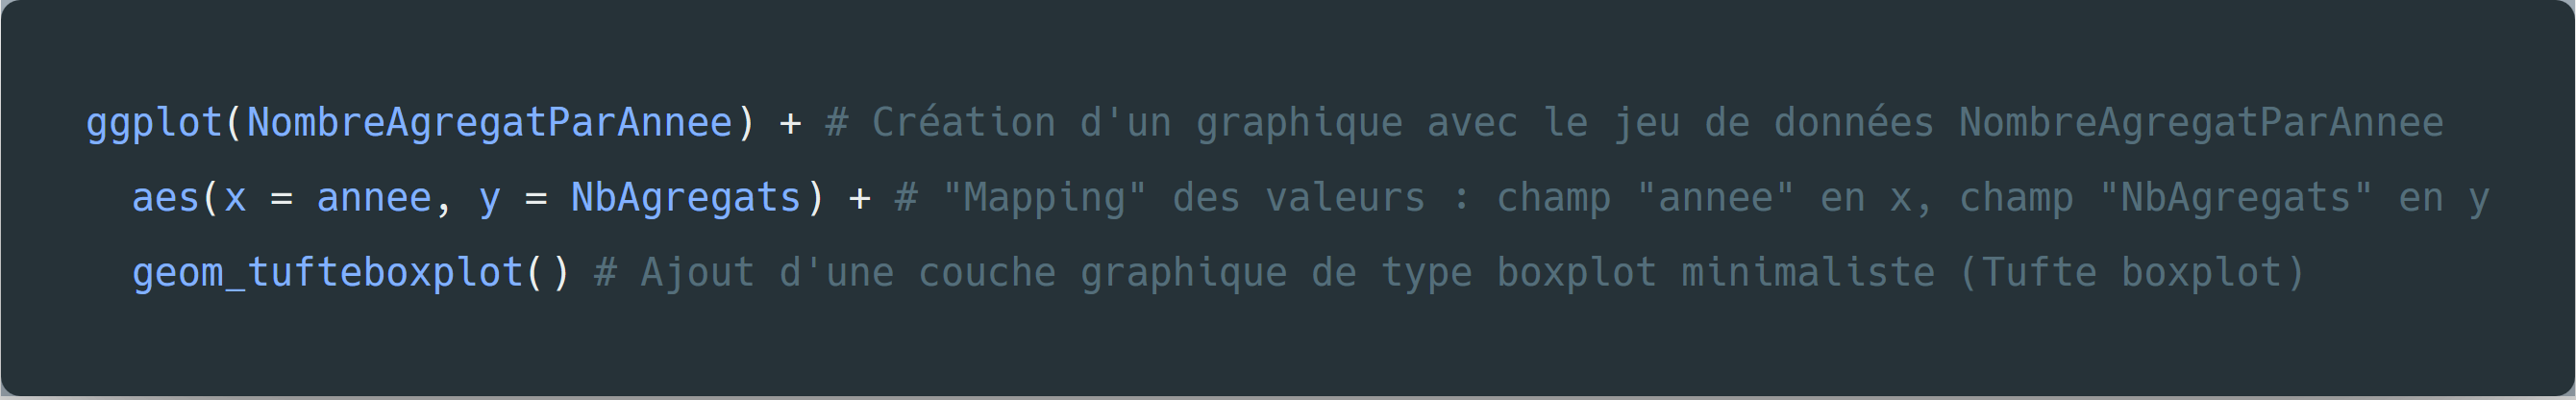
\includegraphics[scale=.15]{img/ggplot2.png}}
				\hspace{5pt}
				\subfloat[Graphique généré]{\label{subfig:exemple-ggplot2-plot}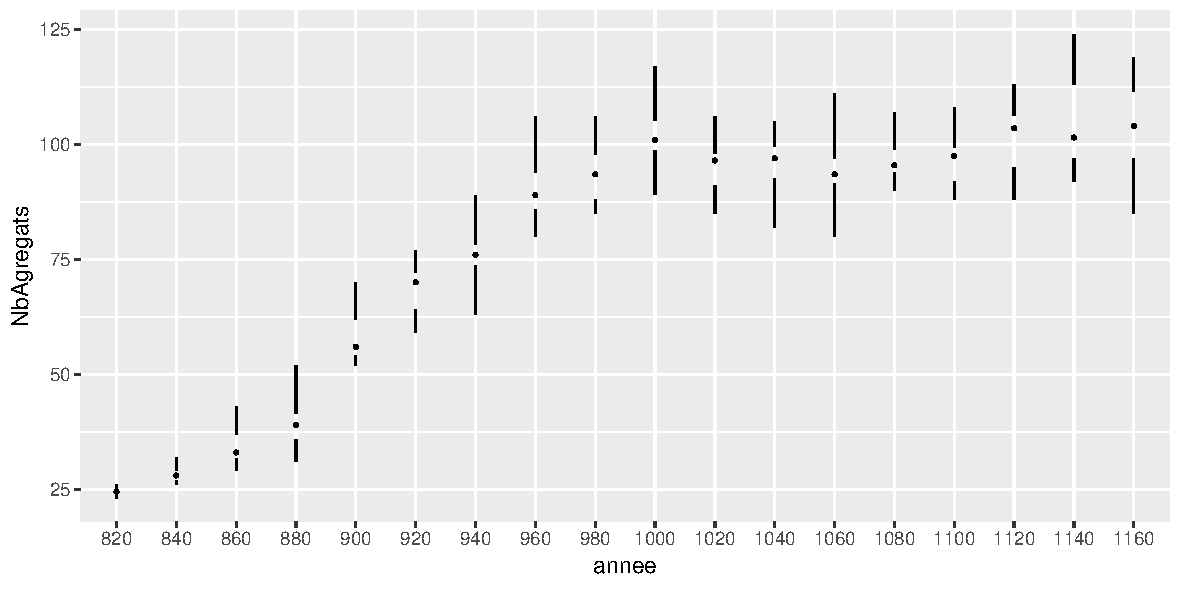
\includegraphics[width=\linewidth]{img/chap5_exemple_indicateur.pdf}}
				\caption{Un exemple de manipulation de données stockées dans un SGBD depuis R.}
				\label{fig:exemple-ggplot2-simedb}
			\end{figure}

	\paragraph*{Fluidifier les étapes de rendu : le \og pipeline de visualisation\fg{}}
	
	
	\Cite{dos_santos_gaining_2004} ont conceptualisé et schématisé l'ensemble des étapes nécessaires à la construction d'une visualisation, depuis les données brutes jusqu'à l'image finale, au sein d'un \og pipeline\fg{} de la visualisation (\cref{subfig:visualisation-pipeline}).
	
	Dans la chaîne de traitement la plus classique, ces étapes s'effectuent au sein de différents logiciels, chacun dédiés à une tâche. Dans le domaine des utilisateurs de SIG, on retrouve par exemple fréquemment une préparation des données dans un tableur, un import dans un logiciel SIG qui va être chargé de la cartographie, puis un export vers un logiciel de dessin vectoriel afin de réaliser la mise en page.
	À chaque changement de logiciel, il est nécessaire d'exporter les données produites, puis de les ré-importer dans le logiciel suivant.
	
	A contrario, le propre de l'utilisation d'un langage de programmation plutôt que d'un outil graphique est de pouvoir automatiser et intégrer l'ensemble de ces étapes.
	L'utilisation de \texttt{R} comme langage de développement de SimEDB nous permet ainsi de développer une unique chaîne de traitement, qui ne requiert aucun import/export de données, et peut donc être consolidée, vérifiée et surtout ré-employée \textit{ad libitum}.
	
	L'enchaînement des \textit{packages} employées dans SimEDB est présenté dans la \cref{subfig:visualisation-pipeline-simedb}, et le code-source correspondant à l'exemple développé dans cette sous-partie dans la \cref{fig:visualisation-pipeline-exemple}.

			\begin{figure}[H]
				\centering
				\hspace{5pt}
				\subfloat[\og \textit{The Visualisation Pipeline}\fg{}, de \cite{keim_mastering_2010}, p.92, d'après \cite{dos_santos_gaining_2004}, p. 314 ]{\label{subfig:visualisation-pipeline}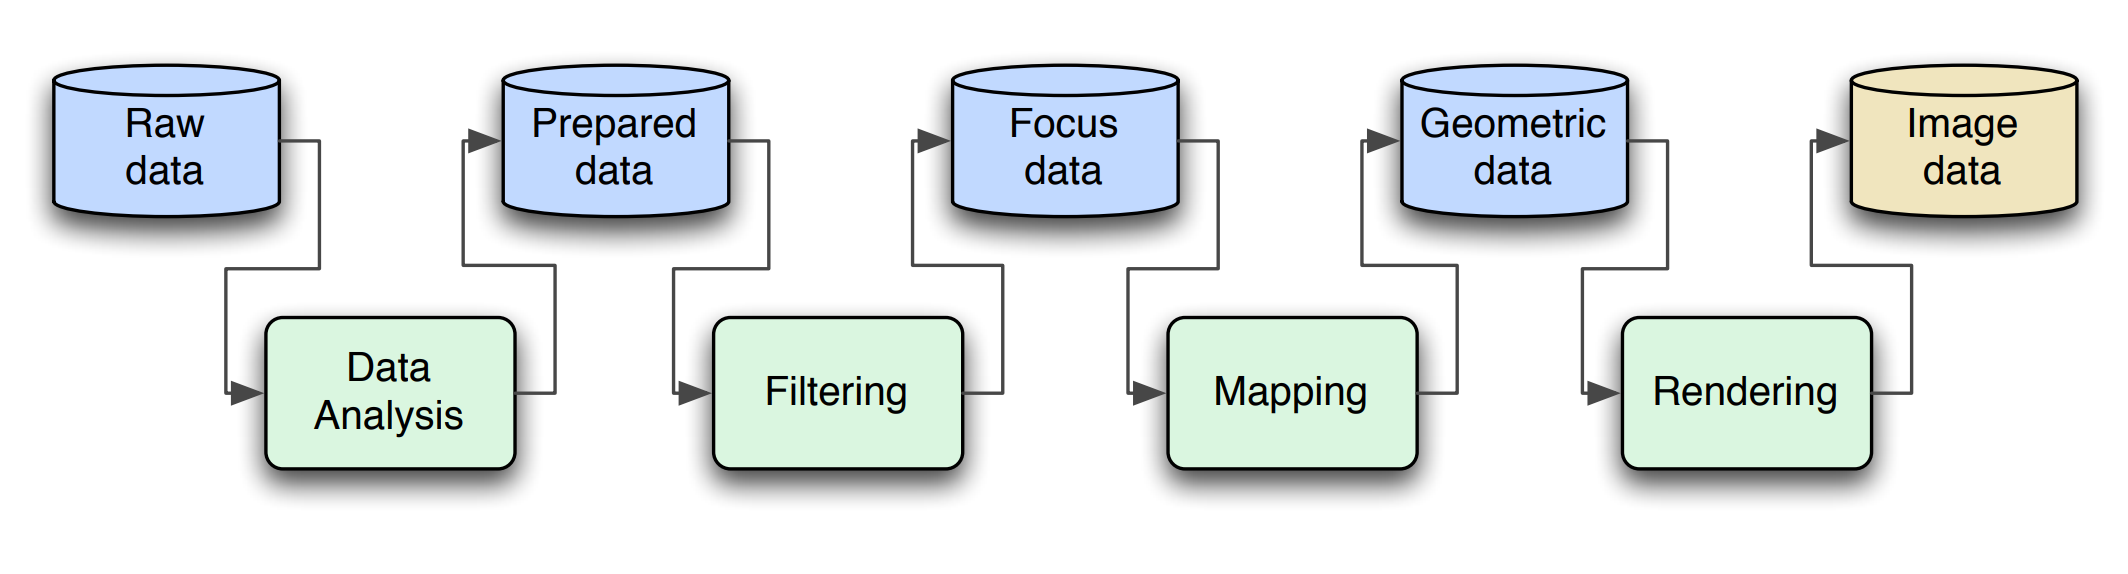
\includegraphics[width=\linewidth]{img/Visualisation_Pipeline_p92.png}}
				\hspace{5pt}
				\subfloat[Technologies utilisées dans SimEDB.]{\label{subfig:visualisation-pipeline-simedb}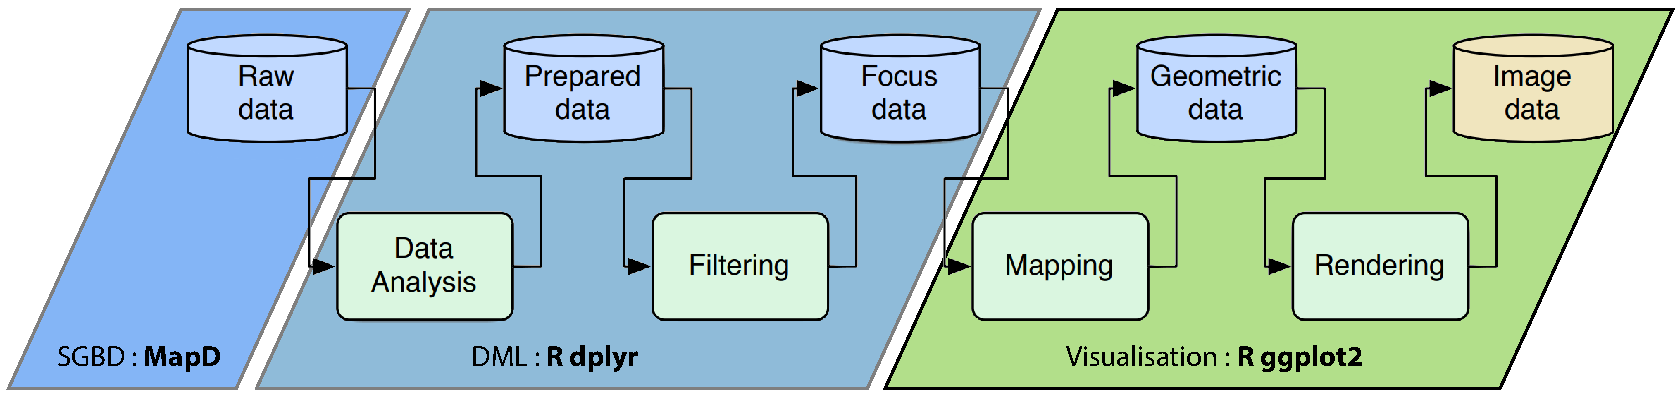
\includegraphics[width=\linewidth]{img/Visualisation_Pipeline_SimEDB.pdf}}
				\hspace{5pt}
				\subfloat[Une implémentation d'un exemple de pipeline de visualisation pour construire un indicateur dans SimEDB]{\label{subfig:exemple-pipeline-simedb}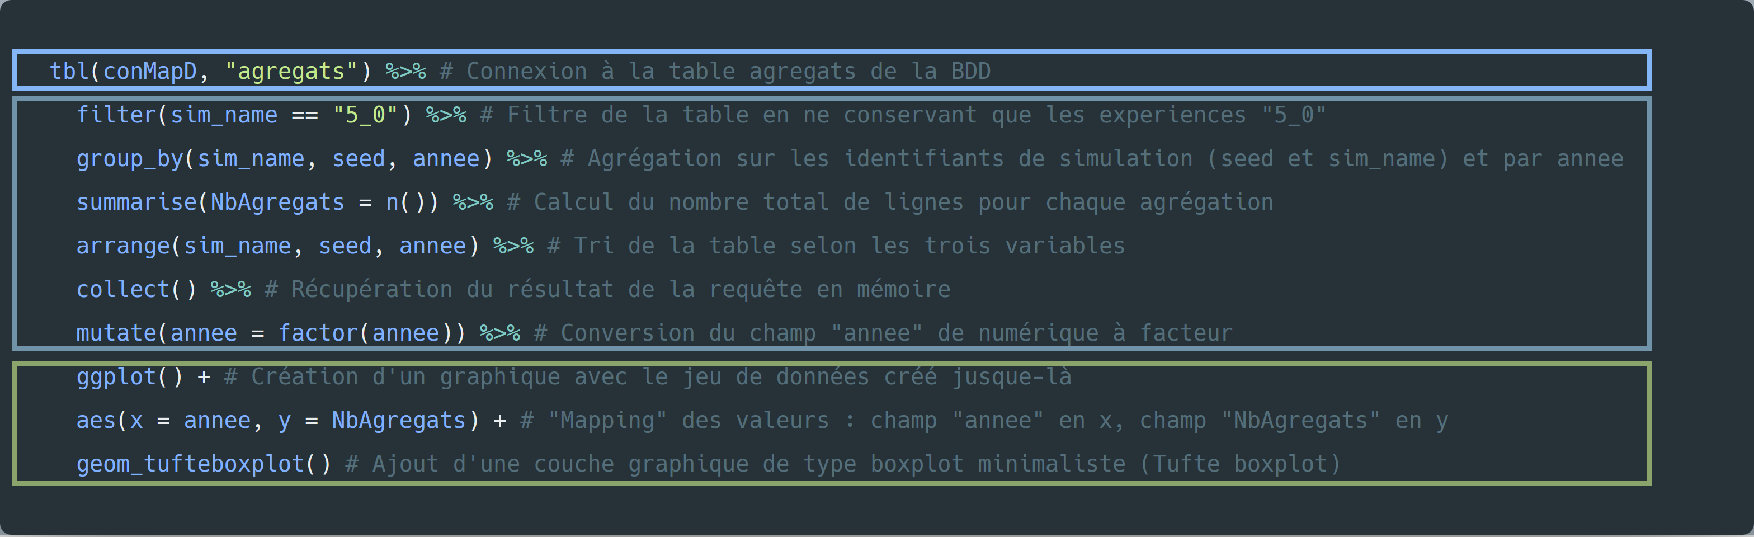
\includegraphics[width=\linewidth]{img/simedb_pipeline_R.pdf}}
			\caption{\og \textit{Visualisation Pipeline}\fg{} et son implémentation dans SimEDB, en \og connectant\fg{} les codes des \cref{fig:dml-simedb,fig:exemple-ggplot2-simedb}.}
				\label{fig:visualisation-pipeline-exemple}
			\end{figure}

			\paragraph*{Modulariser les fonctions}
			
			Shiny, en tant qu'outil de création d'interface graphique, bénéficie aussi d'un avantage important en matière de conception d'application web : comme ce \textit{package} est basé sur un langage de programmation modulaire, on peut logiquement créer et ré-utiliser des \og briques d'interfaces\fg{} modulaires.
			Par l'utilisation de modules\footnote{\href{https://shiny.rstudio.com/articles/modules.html}{https://shiny.rstudio.com/articles/modules.html}}, il est possible de définir un ensemble d'éléments graphiques adaptatifs et de ré-utiliser tel quel cet ensemble.
			
			Dans l'interface de SimEDB, par exemple, les indicateurs graphiques sont toujours présentés de la même manière, avec l'indicateur à gauche et des outils de téléchargement et de notation de l'indicateur sur la droite.
			En termes de code, les deux indicateurs comparés dans la \cref{fig:simedb-modules} sont strictement identiques : seul un paramètre varie dans l'appel aux modules, ici les filtres appliqués sur les données.
			Cela permet donc d'une part de minimiser la taille du code, mais surtout, avec la généricité apportée, de faciliter de manière considérable l'ajout ou la modification d'indicateurs.
			
			\begin{figure}[H]
				\centering
				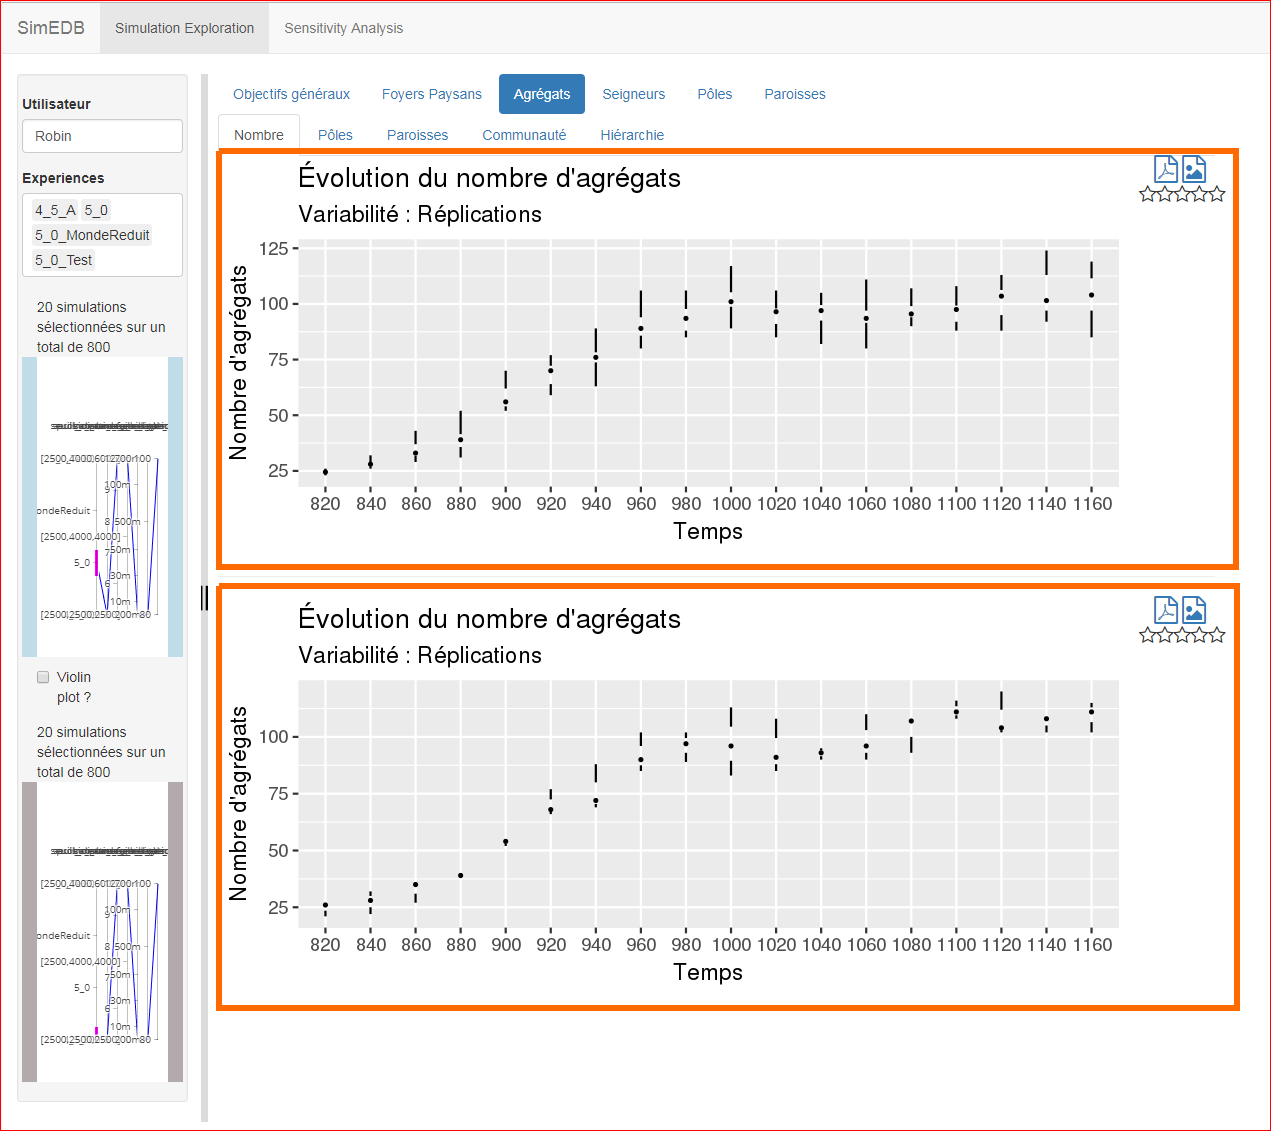
\includegraphics[width=\linewidth]{img/SimEDB_modules.png}
				\caption{Une conception modulaire. Les deux éléments graphiques encadrés sont créés par un même \og module\fg{} dont les arguments varient.}
				\label{fig:simedb-modules}
			\end{figure}


		\subsubsection{Choix de l'organisation visuelle}
		
		Les différentes étapes de construction d'une plate-forme d'exploration (\cref{sec:explorer-sorties-simfeodal} : \cnameref{sec:explorer-sorties-simfeodal}) ont conduit à une organisation sous forme de \textit{dashboard} interactif.
		La forme de ce \textit{dashboard} a évolué tout au long de l'apparition de nouveaux besoins, pour aboutir sur une organisation mono-page, pensée autour de la consultation d'indicateurs de sorties, qui devaient permettre de comparer des expériences différentes sélectionnées au moyen de graphiques en coordonnées parallèles.
		Le choix d'un outil dédié à la comparaison, plus qu'à la visualisation des résultats d'un unique ensemble de simulations, entraîne nécessairement des répercussions en matière de présentation visuelle -- d'interface graphique -- des éléments permettant de mener cette comparaison.
		Depuis la première plate-forme aboutie -- SimVADB (voir \cref{fig:simvadb_dashboard}, \cpageref{fig:simvadb_dashboard}) --, l'interface graphique a donc fortement évolué.
		
			\paragraph*{Une comparaison verticale}
			
			En premier lieu, on peut remarquer que les \og contrôleurs\fg{}, c'est-à-dire les graphiques interactifs en coordonnées parallèles ainsi que de nouveaux menus de sélections (\cref{fig:simedb-sidebar}) ne sont plus dans la partie supérieure de l'interface, mais dans la partie latérale de l'application.
			
			Le choix prédominant à cette modification est la volonté de comparaison : dans SimVADB, on pouvait déjà comparer deux graphiques, mais ceux-ci étaient alors côte-à-côte.
			Étant donné que l'axe des ordonnées est dépendant de chaque graphique -- on ne peut attribuer de limites communes à chaque graphique sans avoir à recalculer chacun des indicateurs à chaque changement de sélection de l'un ou de l'autre --, une comparaison visuelle des positions en ordonnées des courbes et marqueurs n'a pas véritablement de sens.
			Au contraire, le plus souvent, l'axe des abscisses est fixe : qu'il représente le temps (nombre d'agrégats par pas de temps\ldots), une discrétisation de valeurs continues (composition en attracteurs des pôles\ldots), ou encore les différentes modalités d'une variable (détail du déplacement des foyers paysans\ldots), l'étendu et la composition des éléments en abscisse est généralement prévisible.
			
			Avec un axe \og fixe\fg{}, il est donc opportun de mener la comparaison visuelle sur cet axe, et donc d'aligner les graphiques sur celui-ci. L'organisation des différents indicateurs est donc verticale plutôt qu'horizontale.
			
			\begin{figure}[H]
				\centering
				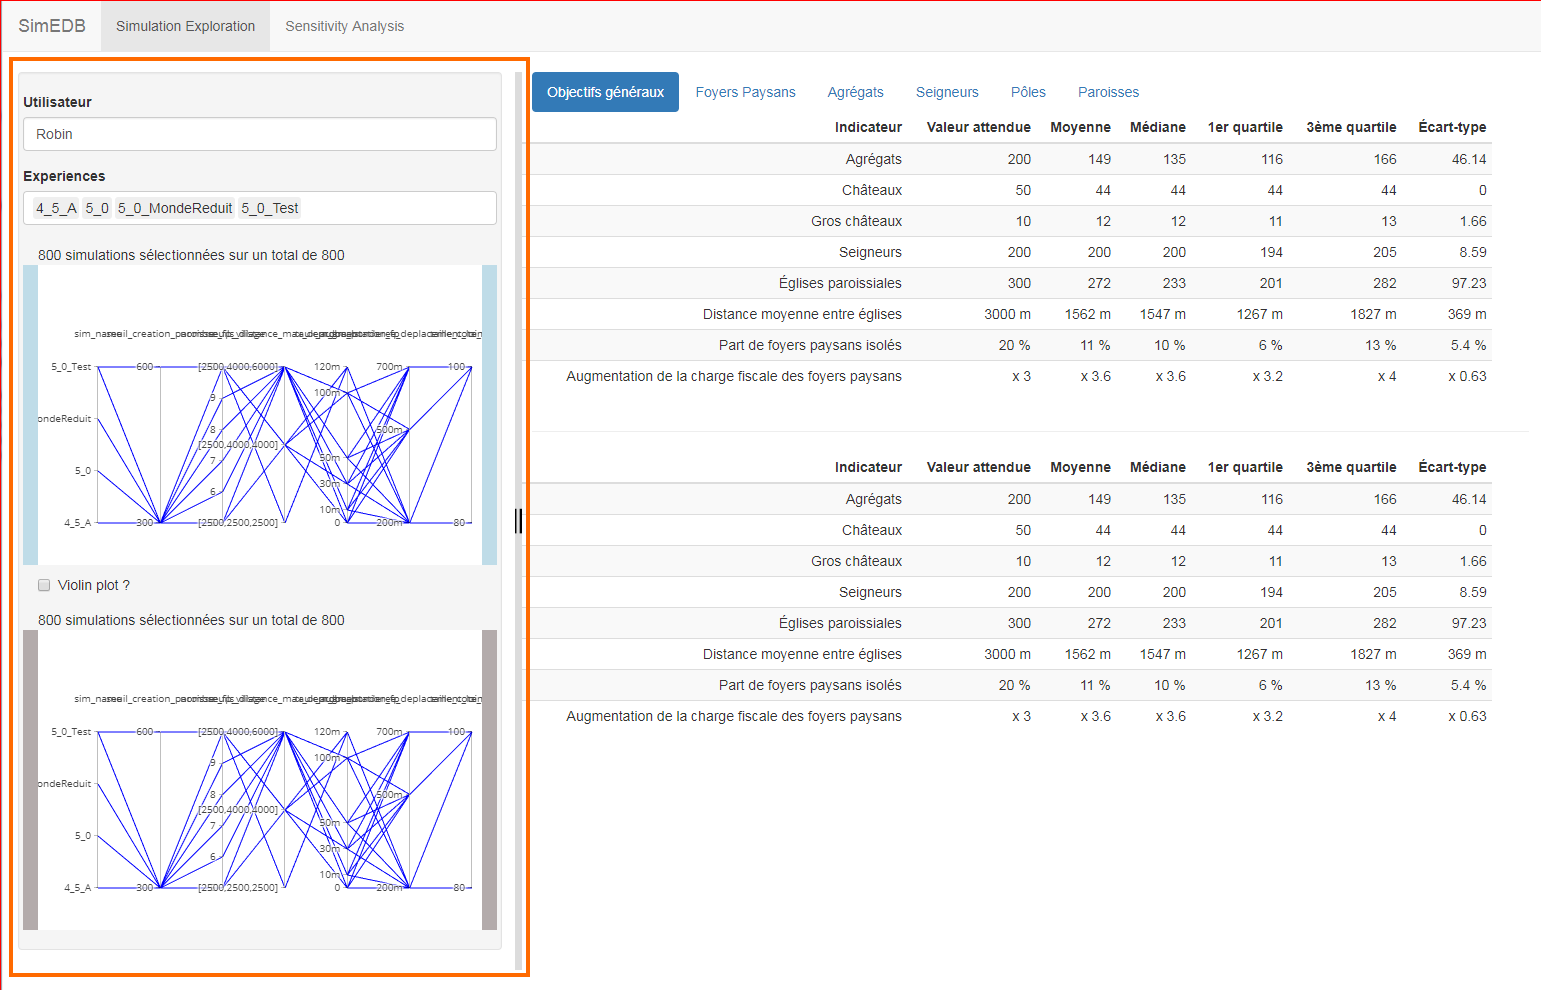
\includegraphics[width=\linewidth]{img/SimEDB_sidebar_cut.png}
				\caption{La barre de contrôleurs dans l'interface de SimEDB}
				\label{fig:simedb-sidebar}
			\end{figure}
		
			Afin que la sélection des simulations à explorer soit intuitive, les contrôleurs doivent donc être alignés face à cet agencement vertical des indicateurs, et dès lors, verticalisés eux aussi.
			
			Pour bien différencier visuellement ce qui relève d'un affichage et ce qui requiert une interaction, les contrôleurs s'inscrivent dans un panneau dédié, grisé, ce qui constitue presque un standard dans les interfaces modernes d'applications interactives.
			
			\paragraph*{Onglets et sous-onglets}
			
			Comme dans SimVADB (\cref{subsubsec:simvadb}, \cpageref{subsubsec:simvadb}), on a choisi de conserver une navigation entre indicateurs par un systèmes d'onglets imbriqués : un premier niveau d'onglets permet d'accéder au type d'agents concernés par les indicateurs, et un second niveau permet de sélectionner spécifiquement l'indicateur choisi.
			On aurait pu privilégier une vision globale, par exemple en affichant d'un coup, pour chaque type d'agents, l'ensemble des indicateurs concernés.
			Sur des écrans de grande dimension, cela aurait permis d'embrasser du regard les résultats propres à chaque type d'agent bien plus rapidement, et d'accélérer d'autant l'évaluation de simulations ou leur comparaison.
			La majorité des utilisateurs potentiels de SimEDB consultent toutefois l'application sur des ordinateurs portables, dotés d'écran réduits et d'une résolution faible.
			L'encombrement visuel est alors atteint rapidement, et mieux vaut présenter un indicateur à la fois : la démarche visuelle sera plus longue, mais ne sera pas gênée ou faussée par des graphiques de dimension trop réduites qui peuvent induire des erreurs de lecture.
			
			L'organisation des onglets en eux-mêmes pose aussi une question importante : vaut-il mieux organiser la consultation par type d'agent, ou plutôt, hiérarchiquement, selon la catégorie de processus examinée (\hl{à corriger une fois fixé sur le terme}, \hl{faire ref au chap3}), par exemple en respectant l'ordre de consultation des indicateurs déterminé ?
			
			Les deux approches présentent des avantages, mais nous avons choisi de rendre l'utilisation de SimEDB plus intuitive à tous, c'est-à-dire en organisant les indicateurs par type d'agents, plutôt qu'efficace, pour les utilisateurs habitués qui auraient bénéficié d'une organisation structurée hiérarchiquement.
			
		\subsubsection{Choix des modes d'interactions}
		
			Avant même la conception de SimEDB, avec la plate-forme SimVADB, nous avions décidé de baser la sélection des simulations sur des graphiques en coordonnées parallèles interactifs (\cref{subsec:explo-interactive} : \cnameref{subsec:explo-interactive}).
			La logique d'ensemble du filtrage de simulations restant la même, il n'était pas nécessaire de modifier ce choix pour SimEDB.
			
			L'accumulation d'expériences, reposant sur les variations de paramètres différents, ainsi que la démultiplication des paramètres du modèle SimFeodal ayant accompagné son paramétrage, ont pourtant demandé de reconsidérer l'usage de ces graphiques interactifs.
			Là où seuls quelques paramètres étaient mobilisés auparavant, les graphiques en coordonnées parallèles reposaient sur peu d'axes.
			Avec l'augmentation du nombre d'axes, le graphique en coordonnées parallèle est rapidement devenu illisible faute à une surcharge graphique due au recouvrement des axes.
			
			\paragraph*{Réduire la surcharge visuelle des graphiques en coordonnées parallèles}
			
			La première mesure pour y remédier a été de filtrer les paramètres affichés : nul besoin d'afficher un axe correspondant à un paramètre qui n'est jamais manipulé dans les expériences.
			Plutôt que de définir les paramètres \og utiles\fg{}, et donc d'avoir à les redéfinir dans l'application à chaque ajout d'expérience qui reposerait sur la variation d'un paramètre différent, nous avons fait en sorte que cette discrimination des paramètres \og actifs\fg{} soit exécutée de manière automatique :
			quand SimEDB est lancé, une requête est exécutée sur la table des paramètres pour identifier ceux qui présentent plusieurs modalités et ceux qui n'en ont qu'une.
			Seuls sont alors affichés les paramètres de la première catégorie, car eux-seuls présent un intérêt à être discriminés.
			
			Ce faisant, le nombre de  paramètre affichés devient plus réduit, et permet d'afficher leurs intitulés plutôt que de faire appel à une table de correspondance comme dans SimVADB.
			L'automatisation de ce traitement permet de plus de ne pas avoir à changer quoi que ce soit à la plate-forme lors d'ajouts ou de suppressions de simulations de la base de données, ce qui concoure à l'objectif d'indépendance aux données de la plate-forme d'exploration.
			
			\paragraph*{Pré-filtrer les simulations}
			
			Au fur et à mesure du paramétrage puis de la calibration de SimFeodal, les expériences ont tout de même continué à mobiliser de plus en plus de paramètres différents.
			Pour réduire la quantité d'information représentée et améliorer en conséquence \og l'expérience utilisateur\fg{}, nous avons ajouté un filtre, moins visuel que les graphiques en coordonnées parallèle, qui permet toutefois de restreindre le nombre de simulations affichées à partir de leur dénomination.
			Plutôt que de cibler des valeurs spécifiques de paramètres, l'idée est donc de soustraire des choix possibles des expériences entières.
			Pour SimEDB, on a donc ajouté un pré-filtrage, sous forme de \og boîte de sélection\fg{} (\textit{select input}, \cref{fig:simedb-prefilter}), qui interroge la base de données directement pour connaître les différents intitulés de simulations et agit comme un premier filtre réduisant donc les simulations interrogées dans les graphiques en coordonnées parallèles.

			\begin{figure}[H]
				\centering
				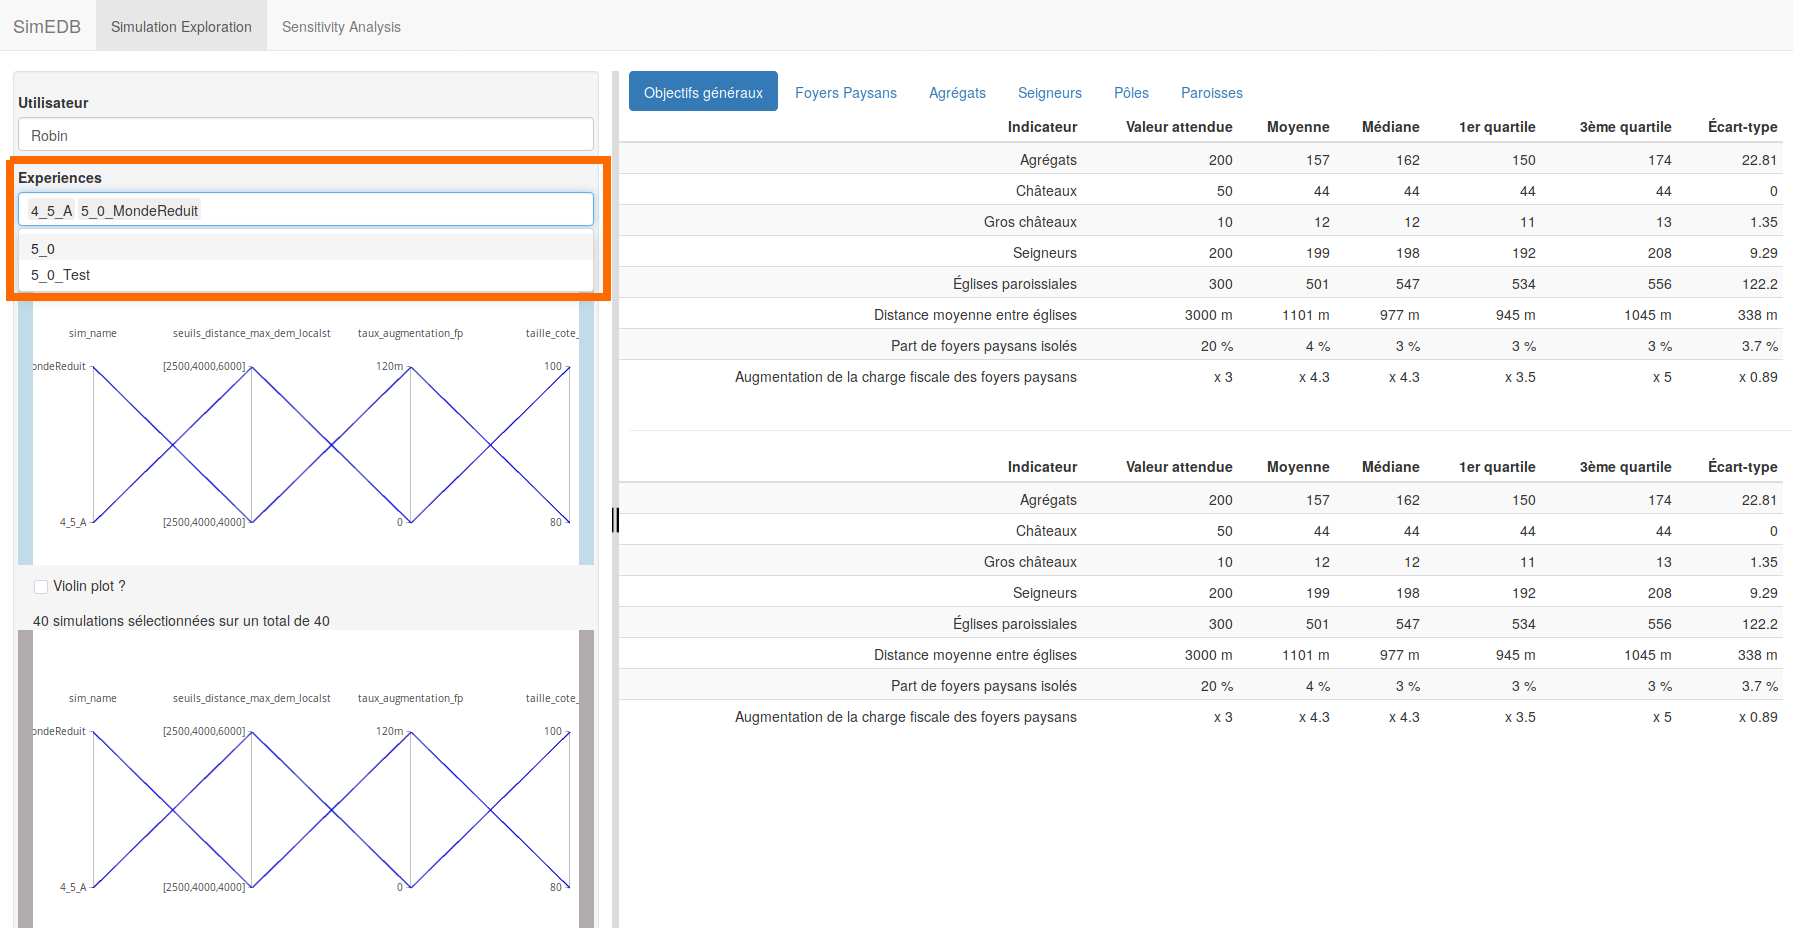
\includegraphics[width=\linewidth]{img/SimEDB_prefiltrage.png}
				\caption{Le menu de sélection des expériences qui permet un pré-filtrage des expériences à partir de leur nom}
				\label{fig:simedb-prefilter}
			\end{figure}
			
			\paragraph*{Optimiser l'occupation de l'espace visuel}
			
			En dépit de ces différentes techniques visant à minimiser le nombre d'axes affichées dans les graphiques en coordonnées parallèles, la place prise par ces graphiques reste importante, en particulier quand on décide de ne pas diminuer la taille des éléments de légende afin de conserver leur lisibilité.
			Quand l'application est consultée sur un écran de taille faible, l'appréhension de l'ensemble des informations présentes dans l'interface pose ainsi un véritable problème.
			
			En réfléchissant aux séquences d'usages, par les utilisateurs, de SimEDB, on a pu comprendre que le mode d'utilisation le plus classique était de bien considérer le filtrage à effectuer sur les graphiques en coordonnées parallèles, en y consacrant un temps certain, avant de comparer longuement les différents indicateurs de la sélection.
			Il n'est donc que rarement fait usage de multiples filtres successifs sur un seul indicateur, dans une approche plus exploratoire donc, mais plutôt d'évaluations complètes de simulations choisies.
			
			Il n'est alors plus indispensable de consacrer une part importante de l'espace aux zones interactives (le panneau de contrôle), ou du moins, pas pendant l'ensemble de la période d'évaluation des simulations.
			
			Un outil de redimensionnement a alors été ajouté à SimEDB, permettant, par glisser-déposer, de modifier la largeur occupée par le panneau de contrôle en l'adaptant à chaque moment au besoin de visualisation.
			La \cref{fig:resizing} montre ainsi une succession d'états : en début d'exploration, l'utilisateur va augmenter la taille du panneau de contrôle pour augmenter la lisibilité des graphiques en coordonnées parallèles et effectuer une sélection plus simplement.
			Une fois la sélection effectuée, il pourra alors re-diminuer la largeur du panneau afin d'augmenter la zone disponible, et donc la taille, pour les indicateurs de sorties de simulation. 
		
			\begin{figure}[H]
				\hspace*{\fill}%
				\begin{minipage}[t]{.49\linewidth}
					\centering
					\vspace{0pt}
					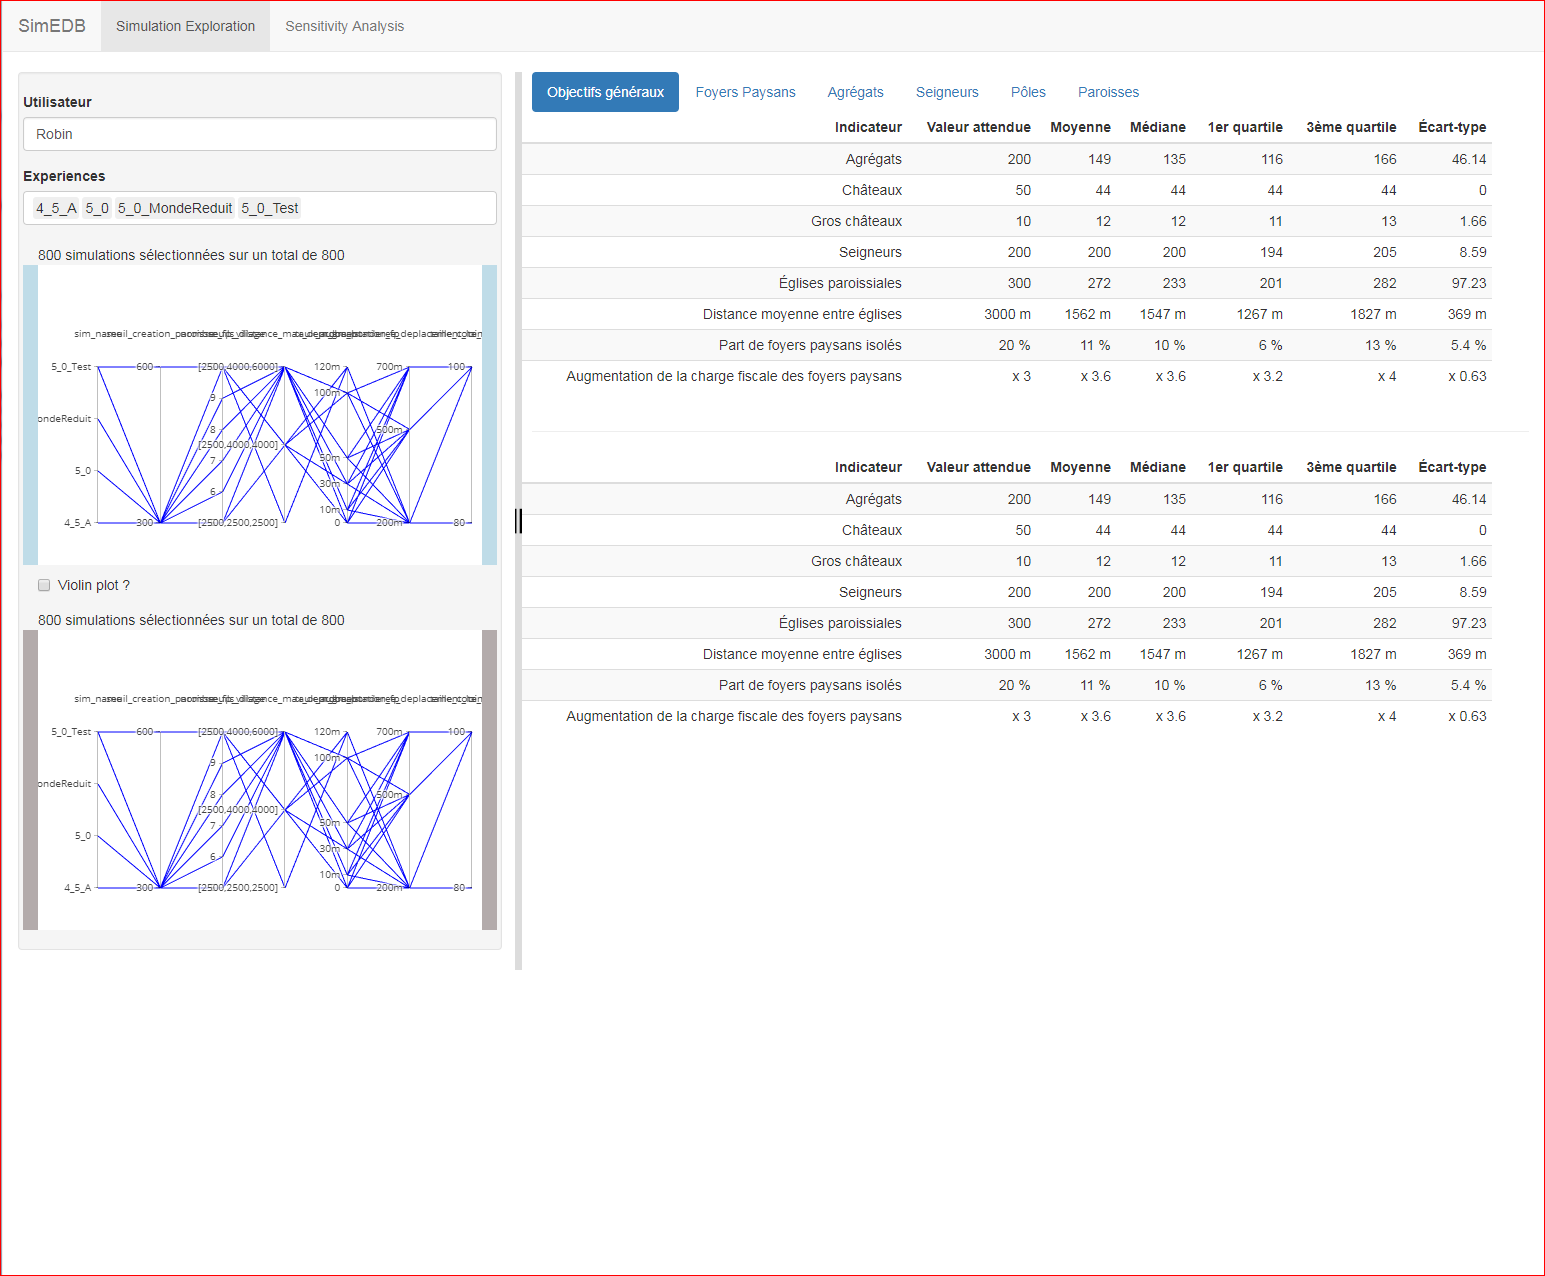
\includegraphics[width=\linewidth]{img/SimEDB_base.png}
				\end{minipage} \hfill
				\begin{minipage}[t]{.49\linewidth}
					\centering
					\vspace{0pt}
					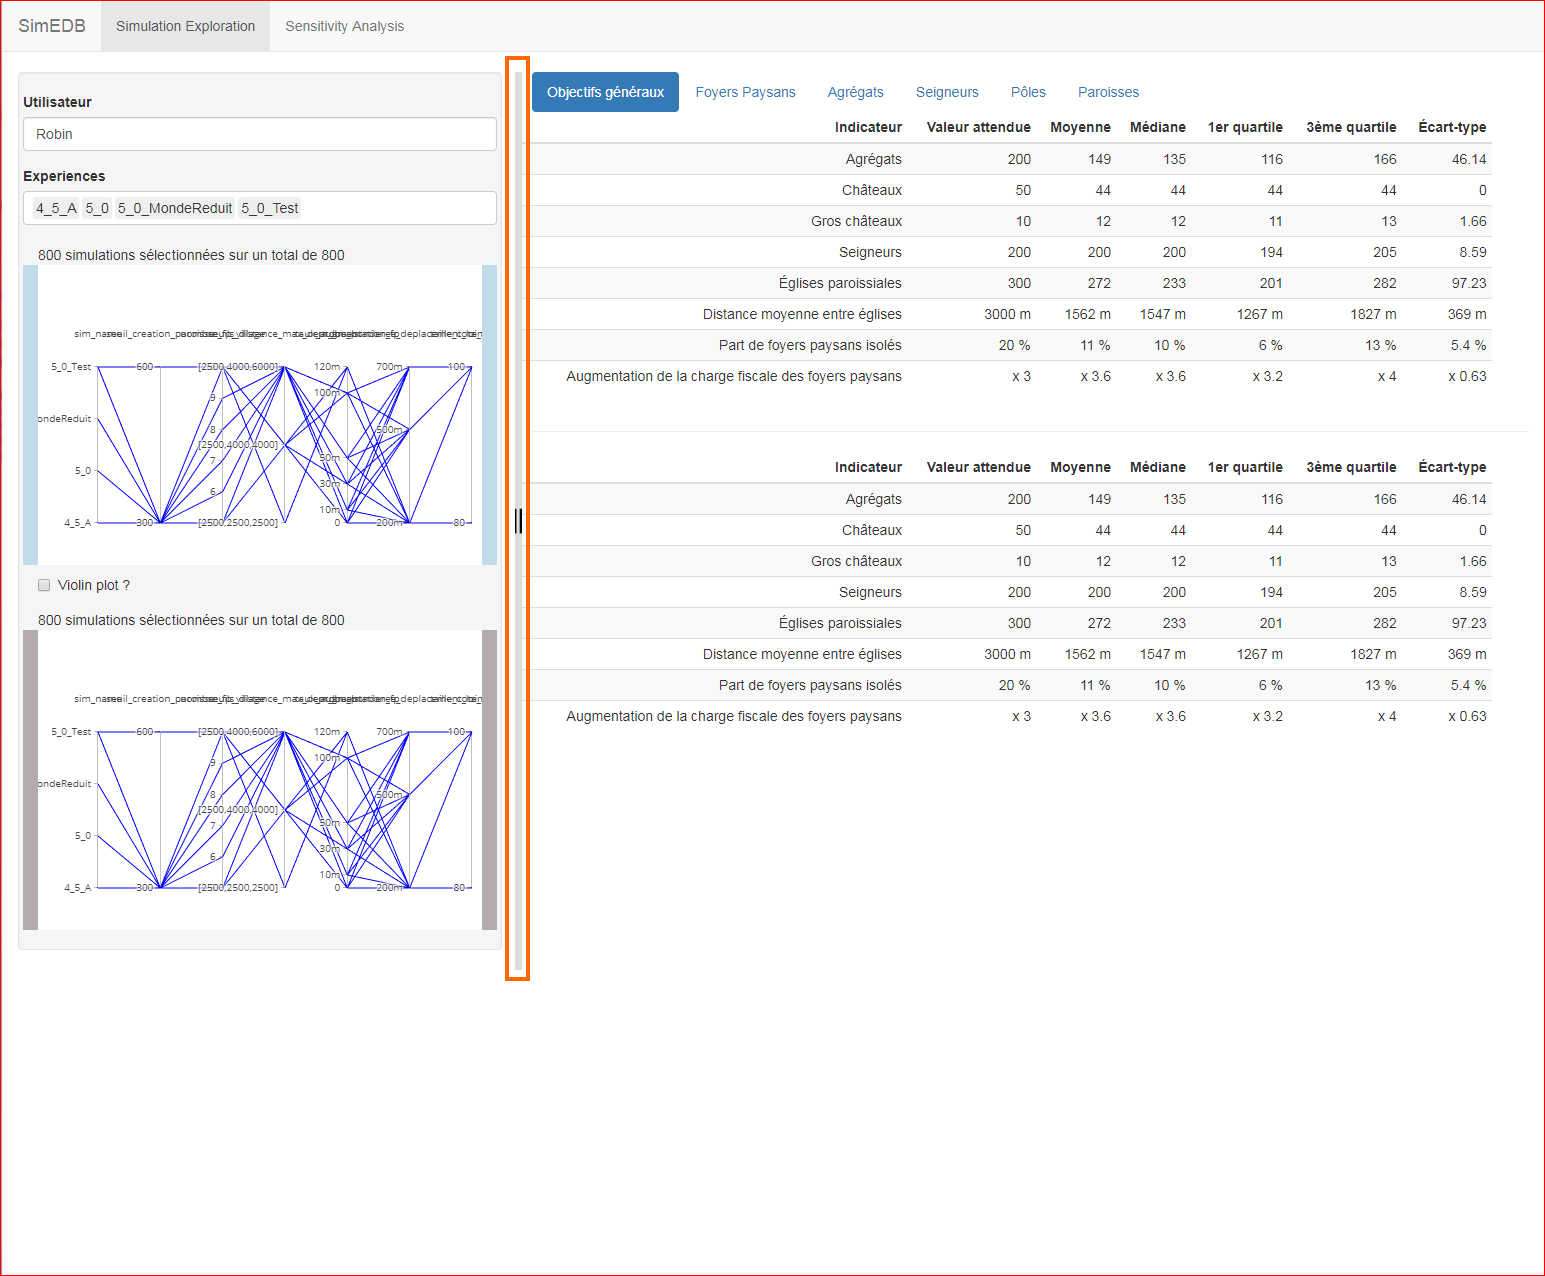
\includegraphics[width=\linewidth]{img/SimEDB_resize.png}
				\end{minipage} \hfill
				\begin{minipage}[b]{.49\linewidth}
					\centering
					\vspace{0pt}
					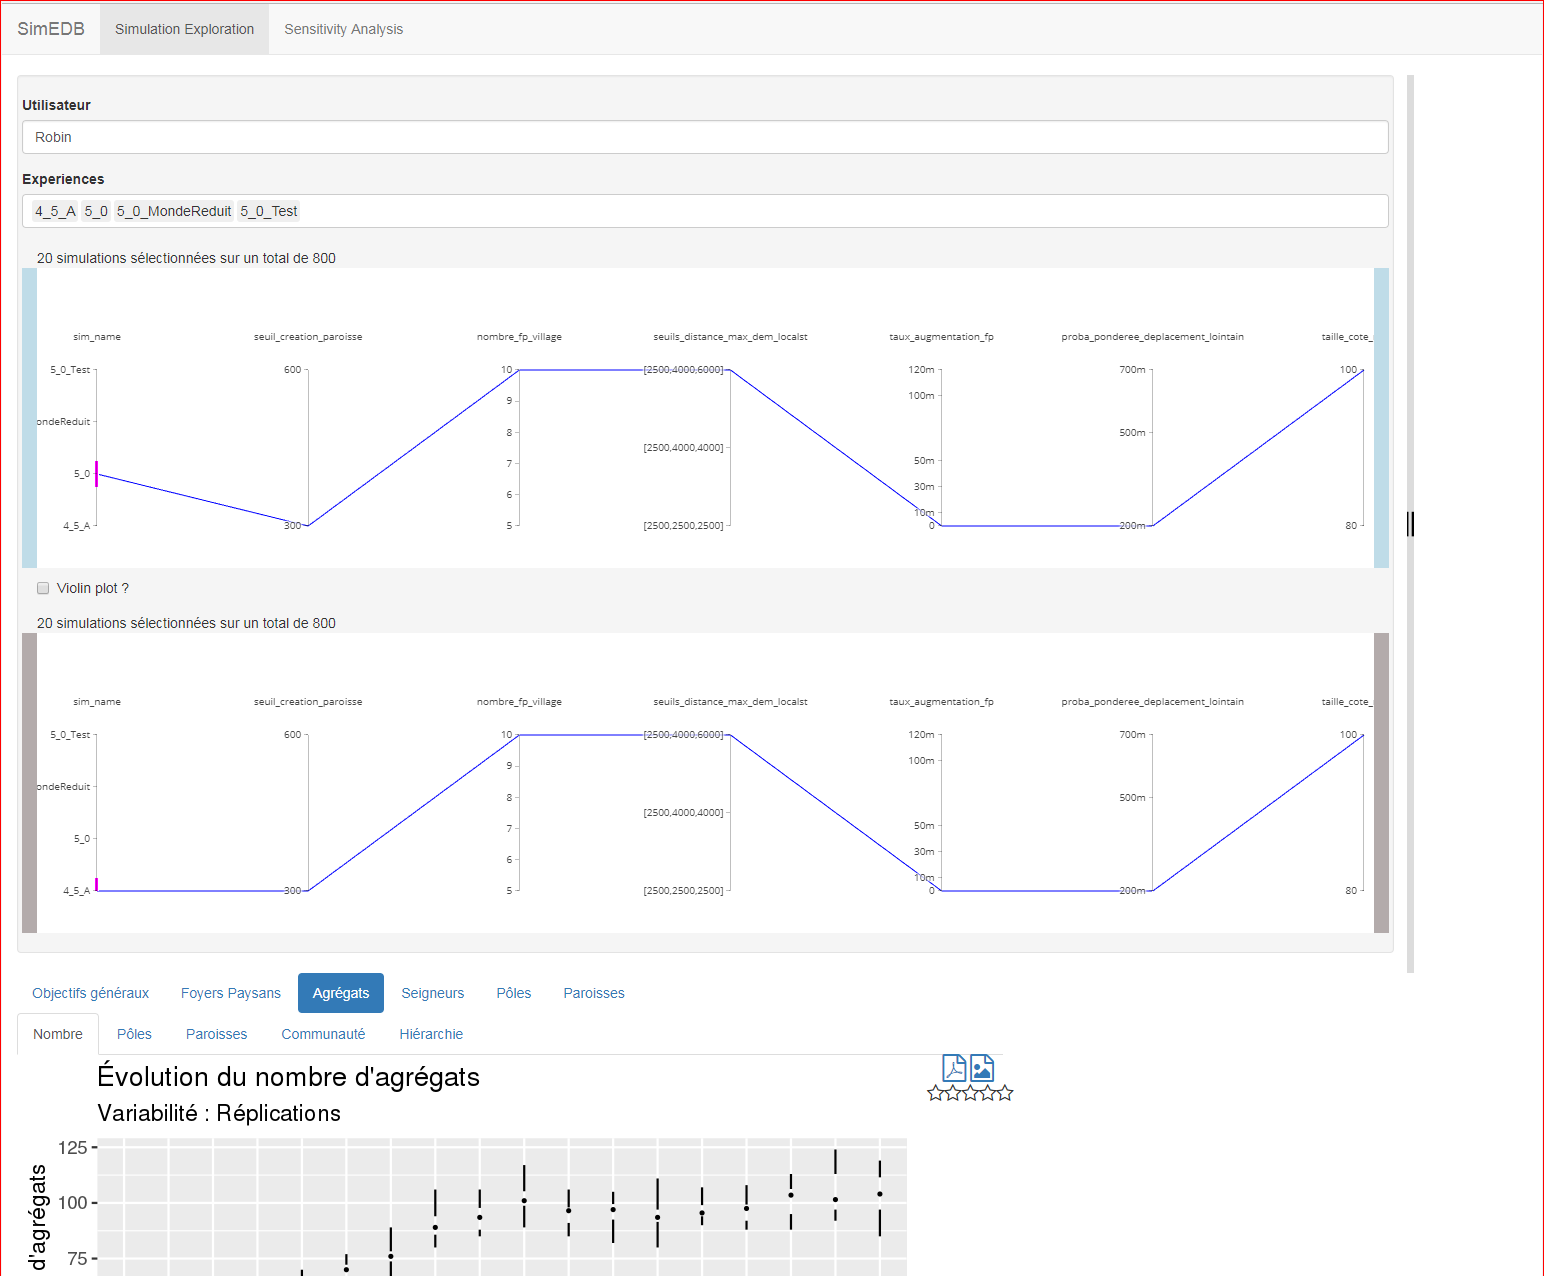
\includegraphics[width=\linewidth]{img/SimEDB_selection.png}
				\end{minipage} \hfill
				\begin{minipage}[b]{.49\linewidth}
					\centering
					\vspace{0pt}
					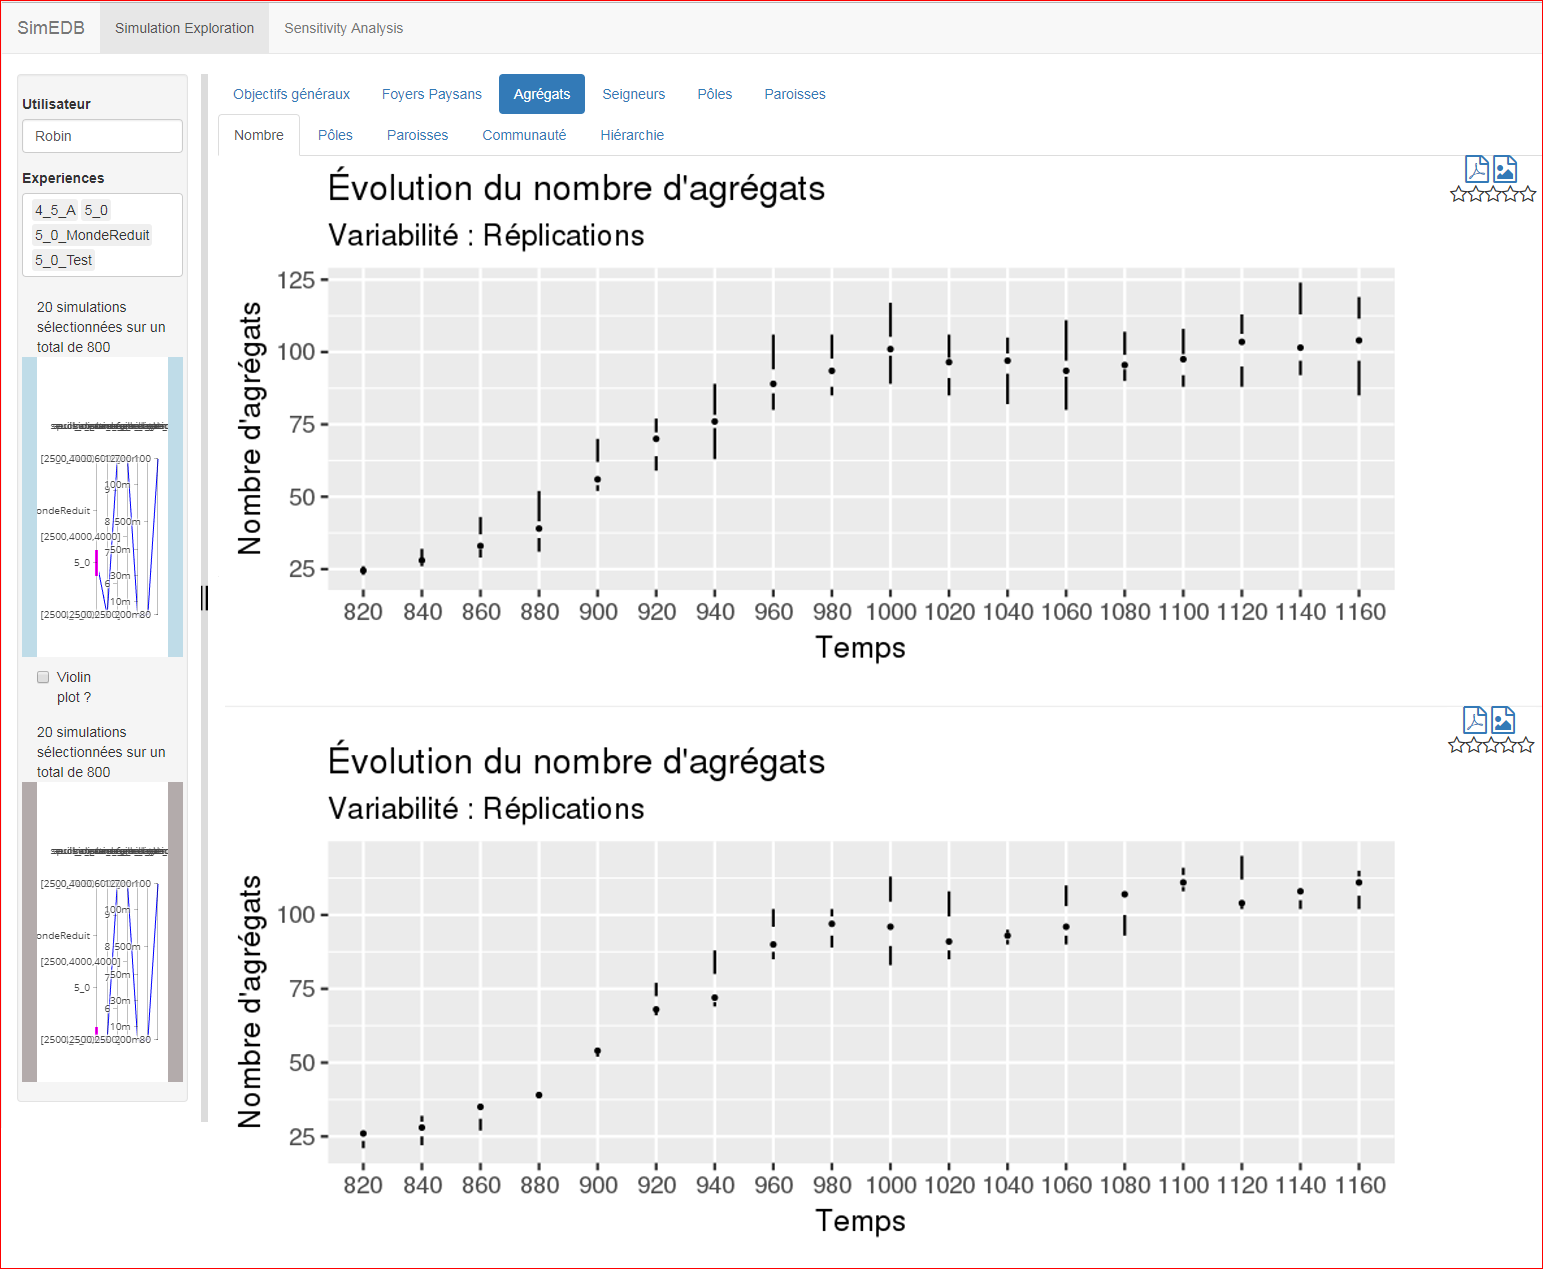
\includegraphics[width=\linewidth]{img/SimEDB_indicateur_grand_magnified.png}
				\end{minipage}
			\caption{Utilisation interactive de SimEDB et redimensionnement du panneau de contrôle.}
			\label{fig:resizing}
			\end{figure}
			
			\paragraph*{Répondre aux demandes des utilisateurs : ajout d'un mécanisme d'export des indicateurs}
			
			L'intérêt d'une interface modulaire et factorisée se révèle véritablement quand les utilisateurs d'un outil demandent des fonctionnalités supplémentaires, non prévues lors de la conception de l'outil.
			Dans le cas de SimFeodal, une telle requête est rapidement apparue : les thématiciens, mais aussi les modélisateurs, pour conserver une trace d'une session d'exploration des indicateurs, souhaitaient pouvoir exporter les graphiques correspondant aux indicateurs.
			Si au départ, une simple capture d'écran pouvait suffire, ce besoin a été complété par une volonté d'inclure des indicateurs de simulations dans des articles et autres communications, requérant donc des retouches des graphiques.
			Pour ce faire, on a choisi d'ajouter des fonctionnalités de téléchargement des graphiques, selon deux formats -- image et vectoriel -- afin de satisfaire à ces deux usages.
			Avec le développement modulaire adopté, il a suffit d'ajouter ces fonctions d'export en un unique lieu dans le code-source de SimEDB, et l'ajout de ces nouvelles fonctionnalités a alors été disponible automatiquement pour chacun des indicateurs graphiques.
			
			\medskip
			\hl{Ajouter un paragraphe, plus tard, sur l'inscription des modalités de filtrage (quelles sont les filtres appliqués ?) dans les graphiques, si j'arrive à trouver le temps de l'ajouter un jour...}
			
			\paragraph*{Noter les simulations}
			
			Un dernier point d'interaction avec l'application a été prévu, sans pouvoir toutefois être mobilisé jusque là : il s'agissait d'aller vers une semi-automatisation de l'évaluation des simulations, par l'intermédiaire d'un outil graphique permettant de \og noter\fg{} les simulations sélectionnées.
			Pour ce faire, et parce que, on l'a vu, l'évaluation d'un ensemble de simulations ne peut se faire de manière unique, on a choisi de donner la possibilité aux utilisateurs experts de noter chacun des indicateurs de sortie, pour chacun des ensembles de simulations qu'ils exploreraient.
			L'évaluation se fait au moyen d'un outil simple, composé de 5 \og étoiles\fg{}, et est enregistré à chaque nouvelle note.
			
			Une piste d'utilisation serait de mobiliser les données ainsi créées, composées d'une note donnée à un indicateur pour un ensemble d'identifiants uniques de simulations, afin de réaliser des analyses quantitatives des notes attribuées : est-ce que certaines simulations sont systématiquement bien notées avec chacun des indicateurs affichés ? Certains indicateurs ne sont-ils jamais observés ou ne donnent-ils jamais lieu à évaluation ?
			
			Cette fonctionnalité, bien qu'implémentée, n'est pas encore utilisée, mais devrait à terme permettre d'aller vers une meilleure connaissance des résultats de simulation, tout autant que vers une mesure de l'efficacité des indicateurs de sortie choisis pour évaluer un ensemble de simulations.

		\subsubsection{Présentation générale}
			 
			 	\begin{itemize}
			 		\item \hl{Quelques captures d'écran successives avec focus à chaque fois sur l'interaction en cours, ou alors,}
			 		\item \hl{renvoyer à un manuel utilisateur en annexe, ou alors,}
			 		\item \hl{ajouter un tuto interactif à l'application et en mettre le lien + descriptif ici}
			 	\end{itemize}
			
	\section*{Conclusion}
	\addcontentsline{toc}{section}{\protect\numberline{}Conclusion}
	
	Au terme de la construction de la plate-forme d'exploration, nous disposons donc d'une application, SimEDB, conçue et développée spécifiquement pour les problématiques propres à l'exploration des données de SimFeodal.
	
	Elle s'inscrit dans les méthodes des Interactions Homme-Machine, ou même dans ce que certains nomment désormais les \og Interactions Homme-Données\fg{} (\og \textit{Human-Data Interaction}\fg{}, \cite{elmqvist_embodied_2011,mortier_human-data_2014}) et s'efforce de suivre les préceptes identifiés dans ce champs (\cite[167-170]{amirpour_amraii_human-data_2018} par exemple).
	
	Le développement a été fortement guidé par les contraintes et besoins identifiées, aussi bien en terme d'approches méthodologiques que de choix technologiques.
	SimEDB est donc un outil \textit{ad-hoc}, toutefois pensé de manière modulaire.
	Tous les composants logiciels de SimEDB sont indépendants et communiquent de manière standardisée, ouvrant la voie à leur remplacement ou \og interchangeabilité\fg{} : l'architecture logicielle et les choix techologiques le permettent.
	La plate-forme SimEDB est donc intrinsèquement pensée comme une réponse à des besoins spécifiques, mais cette réponse a été conçue comme générique et en mesure d'être adaptée aisément à d'autres types de données et/ou sorties de modèles de simulation.
	
	Plus généralement, l'ensemble de ce chapitre montre une démarche similaire, pensée pour répondre à des besoins spécifiques avec des solutions génériques et généralisables.
	Le passage, depuis une succession de rapports jusqu'à une application d'exploration de ces rapports, ou encore les différents éléments relatifs au choix d'un système de gestion de base de données ou au dessin d'un modèle conceptuel de données s'inscrivent en effet dans cette même démarche qui s'ancre profondément dans une logique de recherche reproductible, aussi bien d'un point de vue technique que de celui du concept et de la méthodologie.
	

% Pour compilation finale, décommenter la dernière ligne :
% Permet d'enlever la page vide après le chapitre, mais bloque la création du minitoc. A faire donc après avoir recompilé une dernière fois avec le minitoc
%\let\clearpage\relax
% -> Remplacé pas l'usage de newclude::include*{}

\printbibliography[title={Références}]
